%%%%%%%%%%%%%%%%%%%%%%%%%%%%%%%%%%%%%%%%%%%%%%%%%%%%%%%%%%%%%%%%%%%%%%%%%
%% Official template for the Bachelor's Thesis of the Bachelor AI      %%
%% program of the University of Groningen (NL).                        %%
%%                                                                     %%
%% Current version: March 2026                                         %%
%%%%%%%%%%%%%%%%%%%%%%%%%%%%%%%%%%%%%%%%%%%%%%%%%%%%%%%%%%%%%%%%%%%%%%%%%

\documentclass[10pt,a4paper,twocolumn]{article}
\usepackage{bachelorproject}

% Allow the three methods condition tables to stack at the top of one page
% with text continuing beneath them.
\setcounter{dbltopnumber}{3}
\renewcommand{\dbltopfraction}{0.95}
\renewcommand{\textfraction}{0.05}
\title{\textbf{\textsc{The Stability Gap as a Trajectory Problem: A Bent Descent Path, Its Overshoot, and One Gate in Two Designs}} \\
    \vspace{1ex} 
    \normalsize Bachelor's Thesis\vspace{-2ex}
}

\author{
    \normalsize Arthur Ernst Henrik Reuss, s5582253, a.e.h.reuss@student.rug.nl, \\ 
    \normalsize Supervisor: Gido van de Ven
}

\date{\vspace{-5ex}}


\begin{document}

\onecolumn
\maketitle
\thispagestyle{firststyle}
\begin{abstract}
    \noindent
    Replay-based continual learning is usually judged by the accuracy it reaches \emph{after} each task. Continual evaluation exposes a failure this view hides: the \emph{stability gap}, a sharp but transient drop in past-task accuracy at the start of every new task. The gap persists even when the optimiser descends the exact joint loss over all tasks, so its cause lies in the optimisation trajectory rather than the objective. This thesis explains the gap on two levels. Learning both tasks has a fixed price: the loss on past tasks must rise to its level at the joint optimum. An envelope-theorem argument shows that a reference path exists along which this rise is monotone, so everything the past-task loss does above that level is avoidable in principle. Steepest descent after an abrupt task switch leaves that path: it bows out of the old task's basin and returns from outside, a deterministic arc that survives exact gradients (level one, the trajectory problem). Real optimisers also overshoot whatever path they follow, pushed by an imbalanced first step and by gradient noise from a finite buffer (level two, the overshoot problem). Written in a unified update rule, every replay method counters these problems with the same tool, a \emph{gate} on the new-task gradient, while the replay gradient restores at full strength. We build and compare the two pure gate designs. The \emph{$\lambda$-curriculum} is a scalar feedback gate: it ramps the new-task loss weight up from zero, so the optimiser tracks the moving valley floor of the reference path. \emph{Asymmetric preconditioned experience replay} is a directional feedforward gate: it filters the new-task gradient through past-task curvature, passing it where the past task is flat and braking it where the past task is steep. On rotated MNIST the two levels separate cleanly: removing the overshoot drivers leaves the arc, placing the optimiser on the reference path leaves the overshoot, and doing both removes the gap while the fixed price remains. The curriculum needs momentum: its acceleration repays the plasticity the schedule borrows, and its averaging supplies the variance reduction that closes the residual gap. The directional gate lowers the gap monotonically as its filter strengthens, at no plasticity cost but higher compute; at its strongest setting it fails late and abruptly, consistent with blind spots of its sampled curvature metric, and momentum re-inflates its per-step filter. Which gate wins is therefore set by the momentum regime: without momentum the directional gate is better on both stability and accuracy, but with momentum, which realistic training requires, the scalar gate takes over. On CIFAR-10 with a ResNet-18 the curriculum cuts gap depth several-fold below vanilla experience replay at matched final accuracy and negligible compute cost, under two normalisation schemes and on corruptions it was never tuned on.
\end{abstract}


\clearpage
\setcounter{tocdepth}{2} % sections and subsections
\tableofcontents

\twocolumn

\section{Introduction}
\label{sec:introduction}

Deep neural networks learn rich representations from static, independent, and identically distributed data, but a vulnerability appears as soon as training becomes sequential: the network overwrites previously acquired knowledge to accommodate new data. This phenomenon, catastrophic forgetting \cite{mccloskey:catastrophic, ratclif1990catastrophicforgetting}, is a central obstacle in machine learning: retraining from scratch on all data whenever the distribution shifts is the obvious remedy, but it is too expensive for systems that must adapt continually. Continual learning (CL) studies how to learn from a sequence of tasks without that cost, and its core difficulty is the stability--plasticity dilemma: the model must stay plastic enough to learn new distributions while staying stable enough to preserve old ones \cite{Mermillod2013Stability-Plasticity}.

Several families of techniques address forgetting, including replay, parameter and functional regularisation, optimisation-based methods, and template-based classification \cite{van_de_Ven_2025}. These methods reduce long-term forgetting, but they have historically been evaluated only at task boundaries or at coarse intervals, which hides what happens within a task. Evaluating the network continuously exposes a failure these protocols miss. \citet{delange2023continualevaluationlifelonglearning} did exactly this and identified the \textit{Stability Gap}, a transient but severe collapse in past-task accuracy that occurs immediately upon the introduction of a new task. Even a well-tuned Experience Replay model that finishes a task with high accuracy on earlier tasks passes through a deep minimum during the first hundred steps of the new task.

This matters for three reasons. First, deployed continual-learning systems are queried throughout training, so a model mid-transition commits errors its final checkpoint never would. Second, the transience is a scientific puzzle: the model clearly retains the knowledge needed to recover, so some mechanism must temporarily disrupt and then restore it. Third, relearning what was already known wastes compute, and understanding that mechanism is a prerequisite for fixing the gap efficiently.

The discovery of the gap raised an immediate question: could it be removed by better approximating the joint loss over all tasks? \citet{hess2024complementaryperspectivescontinuallearning} showed that the gap persists even under incremental joint training, where the model has access to all data from all tasks at every step. A perfect objective still produces transient forgetting, so the problem lies not in \emph{what} is optimised but in \emph{how} the optimisation proceeds.

To see why the trajectory itself produces the gap, consider the geometry of sequential optimisation. Figure~\ref{fig:loss_landscape_visualization} visualises a transition from a learned task (Task A) to a new task (Task B), a conceptual two-dimensional reduction of a high-dimensional surface that nonetheless captures the dynamics at play. The network starts at the converged minimum $A$ of Task A and must reach the joint minimum $A\cap B$. Running stochastic gradient descent (SGD) on the joint loss from $A$ follows the green curve: pulled by the steepest gradients of the joint landscape, the trajectory bows outward, leaving Task A's basin and crossing a region of higher Task-A error before converging at $A\cap B$. The dip on Task A along this arc is the stability gap.

\begin{figure*}[htbp]
    \centering
    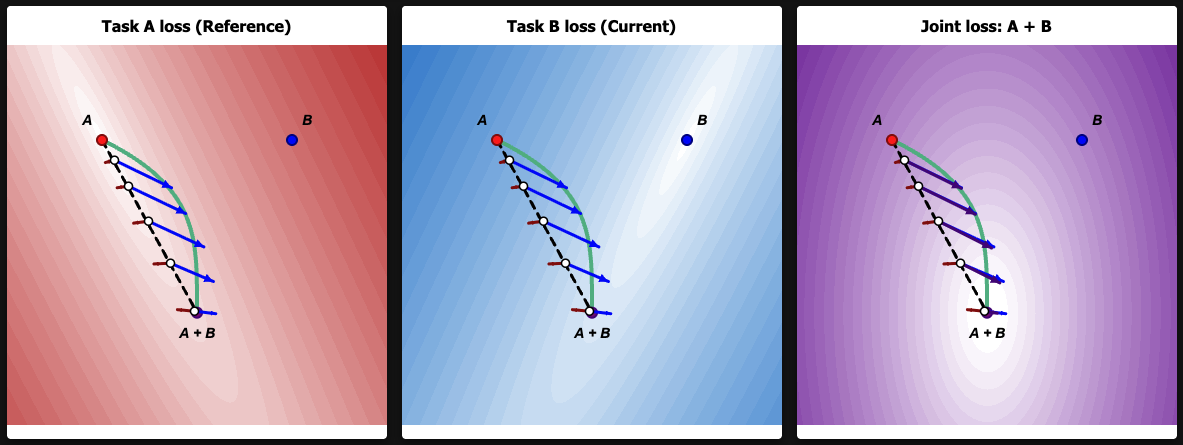
\includegraphics[width=\textwidth]{img/loss_landscape_visualization.png}
    \caption{Conceptual visualisation of the optimisation landscape at a task transition, shown over a shared two-dimensional parameter space. \textbf{Task A} (red) and \textbf{Task B} (blue) are the single-task losses with minima at $A$ and $B$; the \textbf{joint loss} $A+B$ (purple) has its minimum at $A\cap B$. The dashed line is the straight interpolation from $A$ to $A\cap B$; the green curve is the steepest-descent trajectory of the joint loss, which bows away from Task A's basin and induces the stability gap. The fourth panel shows the \textbf{$\lambda$-curriculum} loss $A+\lambda B$: a small weight $\lambda$ on Task B reshapes the basin into a valley that runs continuously from $A$ toward the joint minimum, so the optimum moves along the corridor instead of teleporting across it. Arrows are normalised to a fixed length and show gradient direction only.}
    \label{fig:loss_landscape_visualization}
\end{figure*}

This trajectory is the consequence of a discontinuity at the task boundary. While Task A is learned the optimiser descends the replay loss alone, the red basin in Figure~\ref{fig:loss_landscape_visualization}. The moment Task B begins, the objective switches in a single step to the sum of the replay and current-task losses, the purple joint basin. Its minimum at $A\cap B$ replaces the red one from one step to the next. The parameters do not move during this switch, yet the minimum they are chasing jumps from $\theta_A^*$ to $\theta_{\text{joint}}^*$. We call this \emph{landscape teleportation}: from the optimiser's point of view the surface it was descending disappears and is replaced by another whose minimum lies elsewhere.

The teleportation does more than redirect the optimiser along a curved path; it also makes the very first step after the switch lopsided. At $\theta_A^*$ the replay gradient is near zero, because the optimiser has converged on Task A, while the current-task gradient is large, because Task B is still unlearned. The summed update is therefore dominated by the new-task gradient, and SGD takes a long step out of Task A's basin before the still-negligible replay term can pull it back. This magnitude imbalance compounds the trajectory effect: not only does the descent path bow away from Task A's minimum, the first step along it is the largest and the least opposed, which is why the dip is steepest in the first updates after a task switch \citep{delange2023continualevaluationlifelonglearning}. A finite replay buffer adds a third, smaller error: it estimates the past-task gradient from a handful of stored samples rather than from all past data, so even the replay signal it supplies is noisy. Trajectory effect, magnitude asymmetry, and estimator variance are the three contributors to the gap; Section~\ref{sec:account} makes their decomposition precise and the experiments measure each in isolation.

Existing methods take this discontinuity as given. They accept that the objective jumps at the task boundary and instead make the optimiser robust to the jump, constraining each SGD update with information about the past tasks, their gradients or local curvature, so that SGD avoids directions in which the replay loss rises sharply \cite{lopezpaz2022gradientepisodicmemorycontinual, chaudhry2019efficientlifelonglearningagem, Kirkpatrick_2017, kao2021naturalcontinuallearningsuccess}. We group these approaches under the term \emph{path-finding}: effective as they are, they navigate the broken landscape without removing the break.

This thesis takes the opposite route. Rather than steer the optimiser carefully across a discontinuity, we propose removing the discontinuity itself, an approach we call \emph{landscape-shaping}. We instantiate it as the \textbf{$\lambda$-curriculum}: instead of switching the objective from the replay loss to the joint loss in a single step, the curriculum ramps the current-task loss weight from $0$ to $1$ over the first $N$ steps of each transition,
\begin{equation}
    \begin{aligned}
        L_\lambda(t) & = L_{\text{replay}} + \lambda(t)\, L_{\text{current}}, \\
        \lambda(t)   & = \mathrm{clip}\!\left(\tfrac{t}{N}, 0, 1\right),
    \end{aligned}
    \label{eq:lambda_curriculum}
\end{equation}
so the optimum $\Theta^*(\lambda)$ traces a continuous curve from $\theta_A^*$ (at $\lambda=0$) to $\theta_{\text{joint}}^*$ (at $\lambda=1$), and the model follows this moving valley instead of being teleported across the discontinuity (fourth panel of Figure~\ref{fig:loss_landscape_visualization}). That such a continuous low-loss route from $\theta_A^*$ to $\theta_{\text{joint}}^*$ exists at all is what work on linear mode connectivity \citep{draxler2019essentiallybarriersneuralnetwork, garipov2018losssurfacesmodeconnectivity} establishes: distinct optima are often joined by simple paths of near-constant loss --- the dashed corridor in Figure~\ref{fig:loss_landscape_visualization} --- and the curriculum's role is to keep the optimiser on that route rather than let it bow away. Because the optimum now moves continuously, the curriculum addresses two of the three contributors at once. It removes the trajectory effect, since the descent no longer bows away from Task A's basin (the green curve), and it tempers the magnitude imbalance, since the large new-task gradient is introduced gradually rather than dominating the first step. Only the third contributor, the variance of the finite-buffer estimator, is independent of the schedule and left untouched. Treating the task-boundary discontinuity as the object to be fixed is the central contribution of this thesis; Section~\ref{sec:theory} makes the argument precise.

Two refinements extend the basic curriculum. The linear ramp requires choosing the length $N$; an \textbf{adaptive schedule} removes this knob by setting $\lambda(t)$ from the live ratio of replay to current-task gradient magnitudes. Because that ratio can hold $\lambda$ near zero for the first steps and stall progress on the new task, a \textbf{$\lambda_{\min}$ floor} keeps the current-task gradient present from step one without re-introducing the depth the curriculum removes. Independently, \textbf{momentum} acts as a low-pass filter on the per-step accuracy oscillation that the continuous-limit argument abstracts away, suppressing mini-batch noise while preserving the slow drift along $\Theta^*(\lambda)$.

The remainder of this thesis develops these ideas. Section~\ref{sec:literature} reviews continual learning, Experience Replay, the path-finding methods we compare against, the stability-gap literature, and two lines of work --- blurry task boundaries and mode connectivity --- that bear on the curriculum. Section~\ref{sec:account} then sets out the thesis's own account of the gap: it decomposes the gap into three contributors and contrasts path-finding with landscape-shaping. Section~\ref{sec:theory} proves that a continuous linear $\lambda$-ramp removes the trajectory contributor, with a residual of order $1/N$ in the ramp length. Section~\ref{sec:proposed_approach} states the research questions, and Section~\ref{sec:methods} describes the experimental testbed and the conditions used to test each prediction.

\section{Background and Related Work}
\label{sec:literature}

\subsection{Continual Learning}
\label{subsec:continual_learning}
The introduction described catastrophic forgetting and the stability--plasticity dilemma; here we place the methods that address them. Approaches to forgetting fall into three families \cite{van_de_Ven_2025}. Regularisation-based methods add a penalty that slows changes to parameters identified as important for past tasks, where importance is estimated from a diagonal approximation of the loss curvature \cite{Kirkpatrick_2017}. Architecture-based methods give each task its own parameters, avoiding interference at the cost of a model that grows with the number of tasks. Replay-based methods store a small buffer of past examples and interleave them with new-task data during training. This thesis studies the replay family, and in particular its simplest member, Experience Replay.

\subsection{Experience Replay}
\label{subsec:experience_replay}
Experience Replay (ER) is the simplest replay baseline \cite{chaudhry2019tinyepisodicmemories}. At each step it draws a replay mini-batch from the buffer, combines it with the current-task mini-batch, and takes a single optimiser step on the summed loss of the two. The buffer is populated by reservoir sampling \cite{vitter1985random}, so every sample seen so far occupies a slot with equal probability regardless of arrival order. During $T_0$ the buffer is empty by construction, so ER reduces to plain SGD on the first task, and the stability gap is measurable only from $T_1$ onward.

This simplicity is also why ER remains competitive. \citet{chaudhry2019tinyepisodicmemories} show that jointly training on the current task and a small episodic memory significantly outperforms many purpose-built continual-learning methods. Methods that regularise heavily to protect past tasks tend to give up plasticity, whereas a small replay buffer scales more gracefully to longer task sequences. Consequently, ER serves as a good baseline. Because it does not explicitly manipulate or balance the magnitudes and directions of the gradients, it provides a clean setting to isolate the underlying causes of the stability gap. We therefore adopt it as one of our two core baselines.

A finite buffer is an imperfect estimator of the true past-task distribution. \citet{aljundi2019gradientbasedsampleselection} frame buffer selection as a constraint-reduction problem in which the stored samples approximate the feasibility region defined by the full past data; reservoir sampling is one (non-optimal) policy within that frame. The replay gradient computed on a small buffer therefore differs in direction and magnitude from the gradient on all past data. This estimator gap is present at every step and disappears under no schedule; we report it as a separate, persistent contributor to the stability gap.

\subsection{Path-Finding Methods}
\label{subsec:path_finding}
A second class of replay-based and replay-adjacent methods constrains the SGD update at the task boundary using information about the past tasks. They differ in what information that is. GEM stores past-task gradients and projects the new-task gradient onto the nearest direction whose inner product with every stored gradient is non-negative, so the update does not increase the loss on any past task in the buffer \cite{lopezpaz2022gradientepisodicmemorycontinual}; this uses first-order (gradient) information only. A-GEM replaces the per-task constraints with a single averaged past-task gradient, reducing the projection to one cheap operation \cite{chaudhry2019efficientlifelonglearningagem}. Both act only on the current step, not across the trajectory. EWC instead uses second-order information: it adds a quadratic penalty around the past optimum weighted by the diagonal of the Fisher information, slowing changes to parameters the old task constrained \cite{Kirkpatrick_2017}. NCL also draws on curvature, preconditioning the update by the precision matrix of the past-task posterior to take a natural-gradient step along directions that leave the replay loss roughly unchanged \cite{kao2021naturalcontinuallearningsuccess}. In the framing of this thesis (Section~\ref{subsec:pathfinding_vs_shaping}), all four are \emph{path-finding} methods: they accept the discontinuity at the task boundary and use stored gradient or curvature information to pick a safe trajectory across it. NCL is the second baseline we compare against.

\subsection{The Stability Gap}
\label{subsec:stability_gap}
\citet{delange2023continualevaluationlifelonglearning} introduced continual evaluation and used it to identify the stability gap: the transient accuracy dip on previously seen tasks at the start of new-task training. They observe that the gap is largest in the first few hundred steps of each task, that larger buffers produce smaller gaps, that recovery is partial with the minimum accuracy systematically below the pre-task baseline, and that the gap survives reservoir sampling and moderate learning rates. To explain it, they decompose the update gradient into a plasticity component that lowers the new-task loss and a stability component that preserves the old tasks, and trace the gap to the imbalance between the two at the boundary, where the new-task component dominates. \citet{hess2024complementaryperspectivescontinuallearning} reframe this as a distinction between \emph{what} is optimised and \emph{how}: they show the gap persists even with a perfect approximation of the joint loss, so a better objective alone cannot remove it and the optimisation trajectory must be addressed directly. Subsequent work has shown the gap to be broad rather than incidental: it appears in joint incremental learning of homogeneous tasks \cite{kamath2024expandingscopestabilitygap}, in continual pre-training of large language models \cite{guo2024efficientcontinualpretrainingmitigating}, and in relation to the classification head \cite{lapacz2024exploringstabilitygapcontinual}, and mitigations have been proposed, from temporal ensembles \cite{soutifcormerais2023improvingonlinecontinuallearning} to explicit gap-reduction procedures \cite{harun2024overcomingstabilitygapcontinual}.

\subsection{The Gap Survives the Joint-Loss Oracle}
\label{subsec:kao}
The trajectory argument was made first by \citet{kao2021naturalcontinuallearningsuccess}, who isolate a clean fact about gradient descent through a task transition and illustrate it on a low-dimensional toy problem with two task minima and their combined loss. Remove every replay confound --- no buffer, no sampling noise, no magnitude imbalance --- and give the optimiser exact access to the joint loss $L_{\text{joint}} = L_{T_0} + L_{T_1}$, then run SGD from a stationary point $\theta_0^*$ of $L_{T_0}$. This is the strongest possible replay regime, equivalent to multi-task training with perfect knowledge of the past. Even so, accuracy on $T_0$ dips before recovering. At $\theta_0^*$ the past-task gradient is near zero while the new-task gradient is not, so the first step moves essentially along $-g_1$, where $g_1 := \nabla L_{T_1}(\theta_0^*)$. Writing $H_0 := \nabla^2 L_{T_0}(\theta_0^*)$ for the old-task Hessian, a second-order expansion of the old-task loss gives
\begin{equation}
    \begin{aligned}
        L_{T_0}(\theta_1) - L_{T_0}(\theta_0^*)
         & \approx \tfrac{1}{2}\,\eta^2\, g_1^\top H_0\, g_1 \\
         & > 0,
    \end{aligned}
    \label{eq:kao_taylor}
\end{equation}
whenever $H_0$ has positive curvature in the direction of $g_1$, which it generically does at a strict minimum. The dip is not caused by bad gradients --- the gradient is exact --- but by the \emph{trajectory} the optimiser takes. The conceptual figure in our introduction (Figure~\ref{fig:loss_landscape_visualization}) is drawn in the same spirit; its green curve is precisely this steepest-descent trajectory of the joint loss. This trajectory effect is one of three contributors to the gap, which Section~\ref{sec:account} collects into a single decomposition.

\subsection{Blurry Task Boundaries}
\label{subsec:blurry}
A parallel line of work relaxes the assumption that tasks arrive at sharp boundaries. Standard class- or task-incremental benchmarks present each task as a clean block: all of $T_0$, then all of $T_1$, with an instantaneous switch between them. Several settings replace this with a gradual change. In the \emph{task-free} setting \cite{aljundi2019taskfreecontinuallearning} the learner is never told that a boundary has occurred and the data distribution drifts continuously, so there is no privileged moment at which to consolidate. In the \emph{blurry} setting introduced with Rainbow Memory \cite{bang2021rainbowmemorycontinuallearning} the classes of neighbouring tasks overlap in time: samples of an upcoming class begin to appear before the previous task has ended, so each task shades into the next rather than replacing it. Online formulations push this further, studying blurry, boundary-free streams at the level of individual samples under anytime-inference constraints \cite{koh2022onlinecontinuallearningclass}. Common to all of them is that the transition from one task to the next is spread over many steps instead of one.

This gradual transition is what connects the setting to our intervention, and it makes the blurry-boundary line the closest existing work to the $\lambda$-curriculum. Consider a step on a mini-batch that is an $\alpha$-fraction $T_1$ and a $(1-\alpha)$-fraction $T_0$, with $\alpha(t)$ rising from $0$ to $1$ over the transition window. Its expected gradient is $\alpha\,\nabla L_{T_1}(\theta) + (1-\alpha)\,\nabla L_{T_0}(\theta)$, a weighted sum of the two task gradients. Substituting $\lambda = \alpha/(1-\alpha)$ shows this is, up to an overall scale, the gradient of $L_{T_0} + \lambda L_{T_1}$, the loss the $\lambda$-curriculum descends. A blurry data stream and the $\lambda$-curriculum therefore apply the same fix to the one-sided first step from opposite sides: the former mixes the two task gradients through the \emph{data}, the latter through the \emph{loss weight}. Both keep the past-task gradient present from step one while introducing the new-task gradient gradually.

The two differ in scope. Blurry boundaries achieve the mixing through the data stream and need no buffer, but once $\alpha = 1$ the old-task data, and with it the only retention pressure, is gone; the $\lambda$-curriculum is built on replay and retains an explicit replay signal at $\lambda = 1$. The curriculum is also the cleaner controlled experiment for the stability gap: it changes a single weight in the loss while data sampling, buffer contents, and replay magnitude are held fixed, which isolates the gradual ramp of the new-task gradient as the ingredient responsible for any reduction in the gap. The blurry-boundary results are consistent with ours --- softer transitions forget less --- but, because they vary the data distribution and the loss composition together, they do not separate which of the two is doing the work.

\subsection{Linear Mode Connectivity}
\label{subsec:lmc}

The introduction claimed that a low-loss corridor connects the single-task solution to the joint optimum. Work on \emph{mode connectivity} supports this. \citet{garipov2018losssurfacesmodeconnectivity} and \citet{draxler2019essentiallybarriersneuralnetwork} showed that independently trained minima of a deep network, though separated by a barrier along the straight line between them, are joined by curved paths of near-constant low loss. \citet{frankle2020linearmodeconnectivitylottery} sharpened this to \emph{linear} mode connectivity: networks that share a short period of early training can be joined by a straight low-loss path. For continual learning specifically, \citet{mirzadeh2020linearmodeconnectivitymultitask} found that the multitask solution and the sequentially trained solution often lie in the same basin, linearly connected, when the training regime is stable. This matters for the stability gap in two ways. It means the dip is not forced by the geometry, because a low-loss route from $\theta_A^*$ to $\theta_{\text{joint}}^*$ exists; and it sharpens what an intervention has to do, namely keep the optimiser on that route rather than let it bow away, as the trajectory argument predicts it otherwise will.

Taken together, these results circle the same object from different sides --- the trajectory dip is real and survives an exact objective, softer transitions forget less, and a low-loss corridor to the joint optimum exists --- without naming the mechanism that unifies them. The next section supplies it.
\section{The Stability Gap as a Trajectory Problem}
\label{sec:motivation}

This section reframes the stability gap as a two-level trajectory problem. Learning a new task incurs a permanent stability--plasticity cost; the gap is the transient excess above it. This excess has two sources: a geometric bow in the ideal descent path, and overshoot that real training dynamics add on top. We formalise the split by constructing a monotone reference path, then show that a single design choice, how the update gates the new-task gradient, controls both sources. Two contrasting gates instantiate it: an adaptive scalar curriculum and an asymmetric directional filter.

\subsection{The Permanent Cost and the Monotone Reference Path}
\label{subsec:reference}

Learning a second task inevitably moves the model. In a quadratic approximation with task losses $L_A$ and $L_B$ and Hessians $H_A$ and $H_B$, the displacement $d = \theta_{\text{joint}}^* - \theta_A^*$ from the old optimum to the joint minimum permanently raises the replay loss by roughly $\tfrac{1}{2}\,d^\top H_A\, d$. Every method pays this price; it is distinct from the stability gap.

Yet this rise can be strictly monotone. Consider the curriculum objective $L_\lambda = L_{\text{replay}} + \lambda\, L_{\text{current}}$. As $\lambda$ grows from $0$ to $1$, the minimiser traces a \emph{reference path} $\Theta^*(\lambda)$ from $\theta_A^*$ to $\theta_{\text{joint}}^*$. Under local positive-definiteness, an envelope-theorem argument (Appendix~\ref{app:detailed_proof}) guarantees that the replay loss climbs directly to its final level with no excursion above it:
\begin{equation}
    \frac{d}{d\lambda}\, L_{\text{replay}}(\Theta^*(\lambda)) \geq 0 \qquad \text{for all } \lambda \in [0,1].
\end{equation}

This guarantee is local: it holds only while the combined Hessian $H_A + \lambda H_B$ stays positive-definite along the tracked branch of minima. The condition is automatic near $\theta_A^*$ and persists until the new task's negative curvature overpowers the old task's; on a deep non-convex backbone it therefore serves as motivation rather than a guarantee.

Figure~\ref{fig:lambda_evolution} shows this: as $\lambda$ grows, the loss contours deform continuously from the old-task basin to the joint basin and the minimiser slides along the connected valley floor. Because the replay loss climbs directly to its final level, any transient excess \emph{above} it, the stability gap, is a preventable deviation from the reference path.

\begin{figure}[htbp]
    \centering
    \begin{minipage}[t]{0.31\linewidth}\centering
        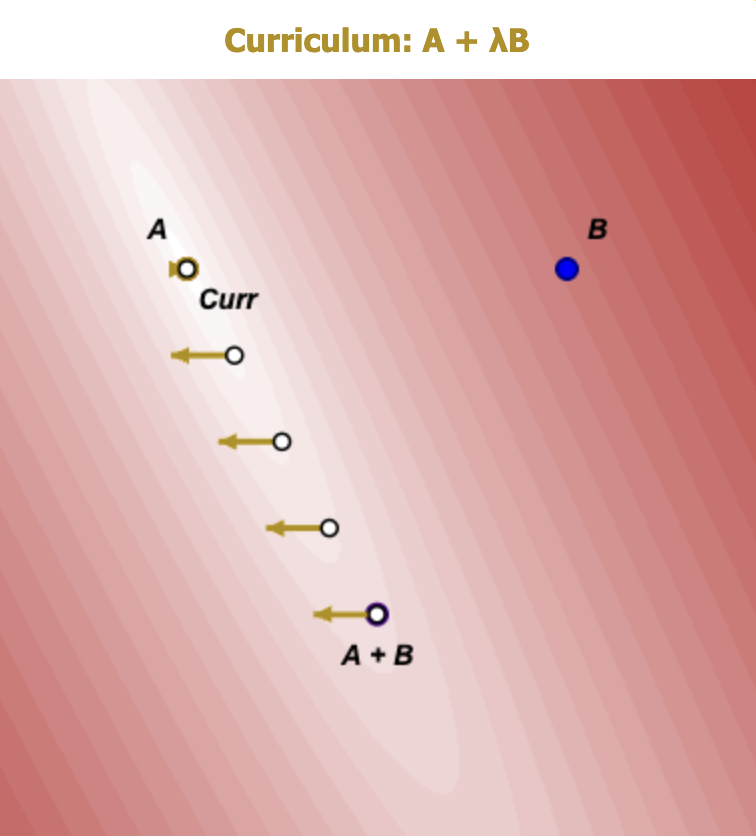
\includegraphics[width=\linewidth]{img/joint_loss_lambda_evolution/joint_loss_lambda_0.png}\\
        {\scriptsize $\lambda = 0$}
    \end{minipage}\hfill
    \begin{minipage}[t]{0.31\linewidth}\centering
        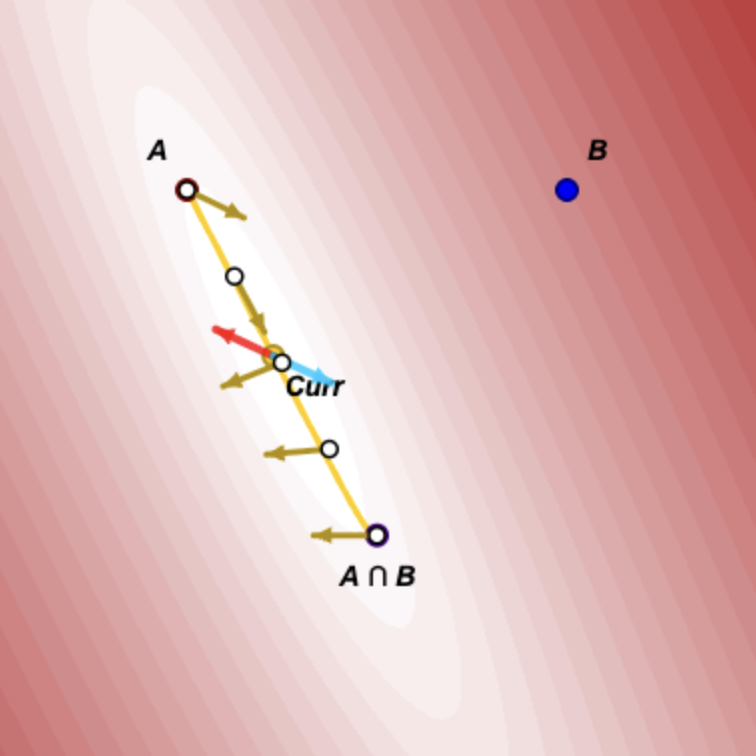
\includegraphics[width=\linewidth]{img/joint_loss_lambda_evolution/joint_loss_lambda_0_025.png}\\
        {\scriptsize $\lambda = 0.025$}
    \end{minipage}\hfill
    \begin{minipage}[t]{0.31\linewidth}\centering
        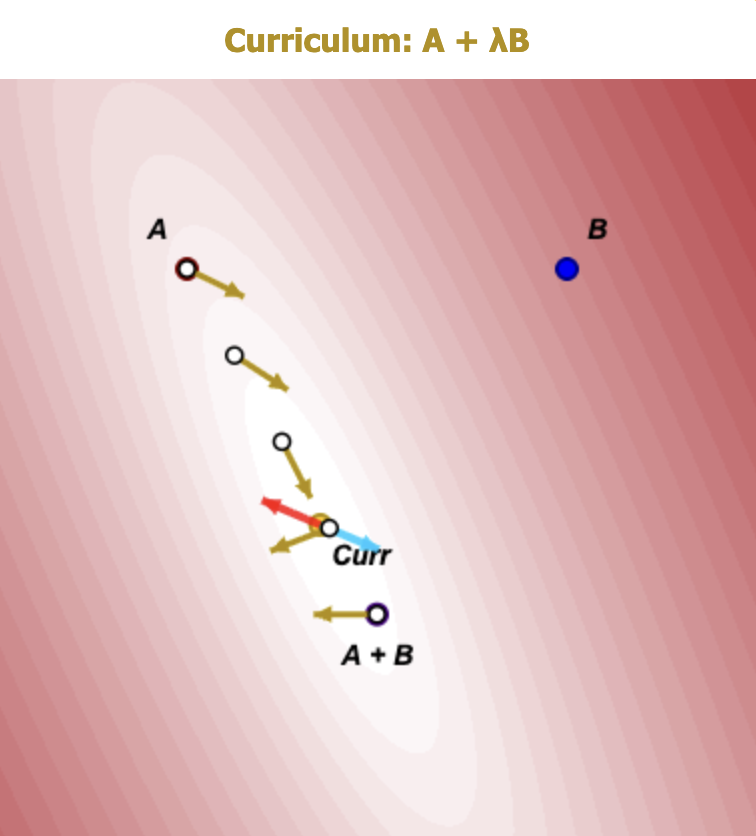
\includegraphics[width=\linewidth]{img/joint_loss_lambda_evolution/joint_loss_lambda_0_07.png}\\
        {\scriptsize $\lambda = 0.07$}
    \end{minipage}

    \vspace{0.5em}
    \begin{minipage}[t]{0.31\linewidth}\centering
        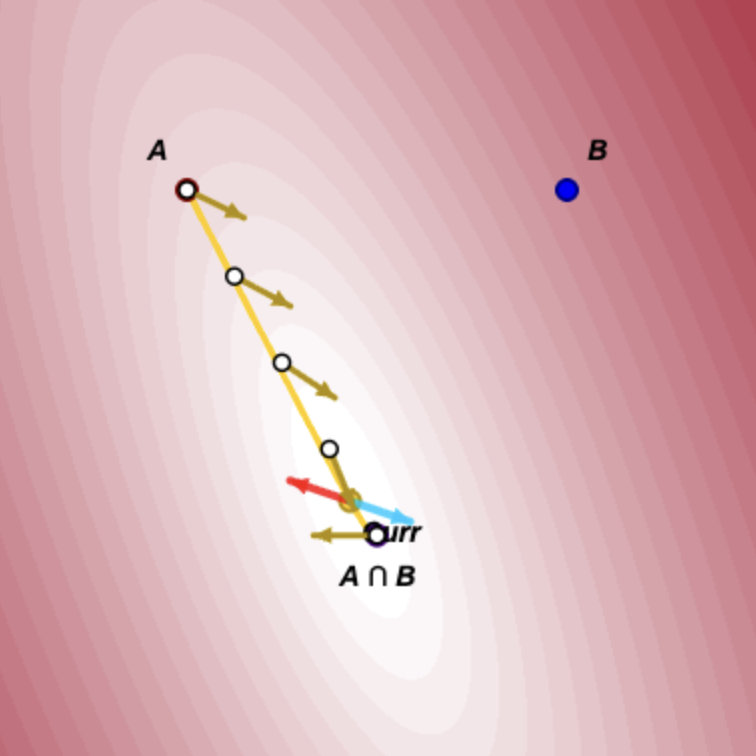
\includegraphics[width=\linewidth]{img/joint_loss_lambda_evolution/joint_loss_lambda_0_175.png}\\
        {\scriptsize $\lambda = 0.175$}
    \end{minipage}\hfill
    \begin{minipage}[t]{0.31\linewidth}\centering
        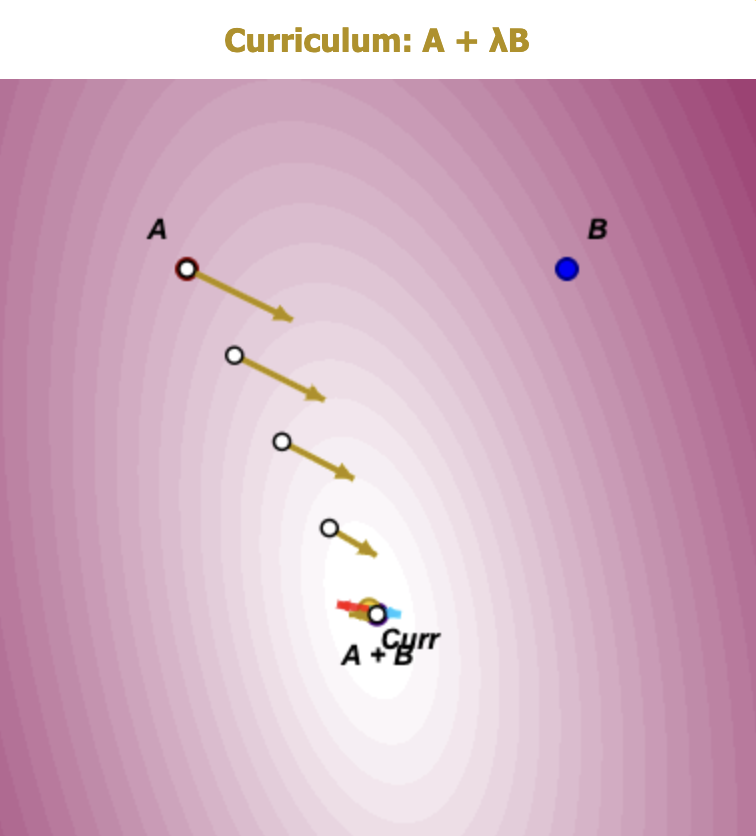
\includegraphics[width=\linewidth]{img/joint_loss_lambda_evolution/joint_loss_lambda_0_5.png}\\
        {\scriptsize $\lambda = 0.5$}
    \end{minipage}\hfill
    \begin{minipage}[t]{0.31\linewidth}\centering
        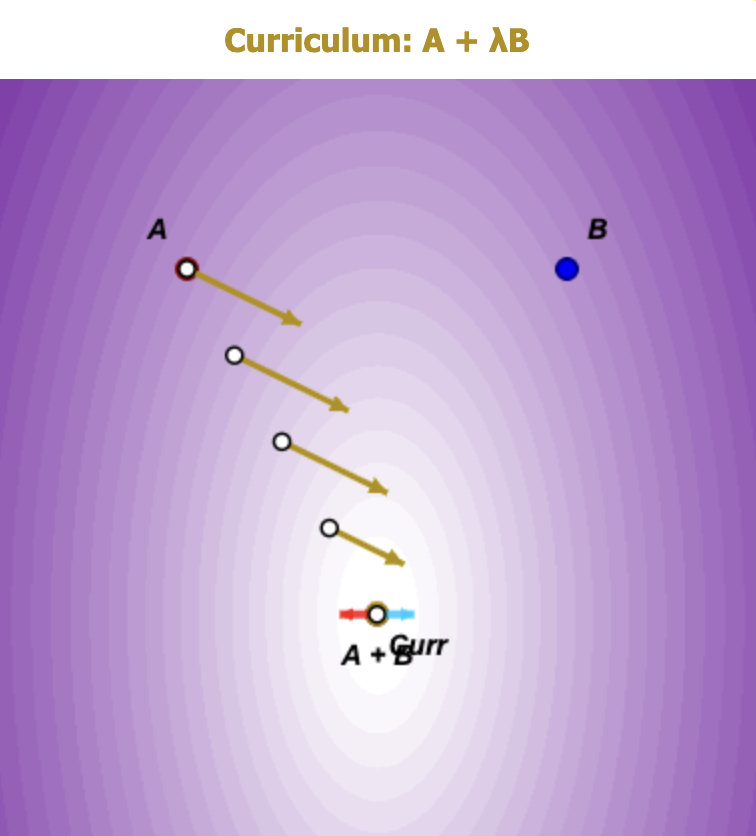
\includegraphics[width=\linewidth]{img/joint_loss_lambda_evolution/joint_loss_lambda_1.png}\\
        {\scriptsize $\lambda = 1$}
    \end{minipage}

    \caption{Evolution of the curriculum loss $L_\lambda = A + \lambda B$. As $\lambda$ increases, the contours morph continuously from the old-task basin around $A$ to the joint basin around $A{+}B$. The current minimiser (\emph{Curr}) slides along the moving valley floor, forming the reference path $\Theta^*(\lambda)$. At the minimiser, the replay (red) and current-task (blue) gradients cancel; the joint gradient (golden) vanishes at the minimiser and points down the valley, ensuring a tracking model rides the floor instead of teleporting across the landscape.}
    \label{fig:lambda_evolution}
\end{figure}

\subsection{The Two-Level Gap: Bowing and Overshoot}
\label{subsec:trajectory_problem}

Real trajectories deviate from the reference path on two distinct levels.\\

\textbf{Level One (The Bow):} Even under highly idealised conditions (exact gradients, vanishing step size), the steepest-descent direction of the abruptly assembled joint loss misaligns with the direction toward the joint minimum whenever the loss curves more sharply in some directions than in others. The trajectory bows outward, leaving the old task's basin before returning \citep{kao2021naturalcontinuallearningsuccess}. This deterministic out-and-back arc forms the structural core of the gap (Figure~\ref{fig:loss_landscape_visualization}, green curve).\\

\textbf{Level Two (Overshoot):} Real training dynamics inflate this arc. At a sudden task boundary, the minimum teleports from $\theta_A^*$ to $\theta_{\text{joint}}^*$, leaving the iterate exposed to a large new-task gradient while the replay gradient is near zero \citep{delange2023continualevaluationlifelonglearning}. Two acute drivers, finite step sizes and momentum accumulation, amplify this unopposed push, creating the sharp first-step drop. Concurrently, a chronic driver, estimator variance from finite buffer sampling (Section~\ref{subsec:experience_replay}), injects noise that delays the slow recovery tail.\\

\textbf{The Tracking Bound:} Stretching the transition over an $N$-step ramp resolves both levels at once. Introducing the new task slowly ($\lambda \approx 1/N$) makes the reference path of Section~\ref{subsec:reference} the path the dynamics actually define, so the bow disappears; and it keeps the iterate tethered to the moving valley floor $\Theta^*(\lambda(t))$ rather than leaping across the landscape, with a tracking lag that a gradient-flow analysis bounds by $O(1/N)$ (Appendix~\ref{app:detailed_proof}). The two combine to cap the highest transient replay loss during the transition:
\begin{equation}
    \max_t\, L_{\text{replay}}(\theta(t)) \;\le\; L_{\text{replay}}(\theta_{\text{joint}}^*) + O\!\left(\frac{1}{N}\right),
    \label{eq:bound}
\end{equation}
where the first term is the permanent price of Section~\ref{subsec:reference} and the second is the transient, which shrinks with ramp length. This continuous-limit argument controls the deterministic arc and the acute overshoot, but the per-step stochastic noise of the buffer survives any ramp length and requires a separate remedy, addressed in the momentum experiments of Section~\ref{subsec:momentum}.

The two levels partition the gap's two dimensions: the acute drivers set the depth of the initial drop, while the hanging tail is the Level-One arc plus the slow, noisy recovery the chronic driver leaves behind. This yields the falsifiable core tested as RQ1: removing the overshoot drivers should flatten the drop and leave the arc, placing the optimiser on the reference path should remove the arc and leave the overshoot, and doing both should close the gap while the permanent cost of Section~\ref{subsec:reference} remains.

\subsection{Two Gates: Attenuating the New-Task Gradient}
\label{subsec:gates}

Equation~\eqref{eq:unified_update} shows that replay methods differ mainly in how they weight the replay and current-task gradients. The replay gradient is the only restoring force pulling the iterate back to the reference path, so a protective method must attenuate the new-task push---the source of the bow and overshoot---while leaving the restoring gradient intact. Generalising the current-task weight to an operator $G$ yields a one-sided \emph{gate}:
\begin{equation}
    d \;=\; G\, g_{\text{cur}} \;+\; g_{\text{rep}}.
    \label{eq:gate}
\end{equation}

The curriculum of Section~\ref{subsec:reference} realises this gate along one axis, \emph{time}: it introduces the new task slowly, so the push is never large enough at once to knock the iterate off the reference path. A complementary axis is \emph{direction}. At any single step only part of the push is harmful, because the past task is flat in most directions and steeply curved in a few, and only motion along the steep directions raises the replay loss. Preconditioning the push by past-task curvature exploits this, passing it at full gain where the past task is flat and shrinking it where the past task is steep, so retention costs little plasticity. This natural-gradient idea underlies Natural Continual Learning \citep{kao2021naturalcontinuallearningsuccess} and, in a replay setting, Online Curvature-Aware Replay \citep{urettini2025onlinecurvatureawarereplay}. Both, however, precondition the \emph{entire} update, so the same metric that brakes the harmful push also brakes the restoring replay gradient---protecting the past task only by slowing the return to it. Asymmetric PER keeps the gate one-sided: it filters the new-task gradient alone and leaves the restoring gradient at full strength. We include the symmetric preconditioner, which damps both, as a control (Appendix~\ref{app:per_sym}).

As detailed in Table~\ref{tab:gates}, gates vary by their \emph{domain} (scalar vs.\ directional) and \emph{control} (feedback vs.\ feedforward). This thesis explores the two pure corners of this design space:

\begin{description}
    \item[Adaptive $\lambda$-curriculum (Scalar Feedback):] A scheduling parameter $\lambda(t)$ sets the new-task weight from the ratio of replay to new-task gradient norms. By scaling the loss itself, it deforms the objective into the homotopy of Section~\ref{subsec:reference}, so the optimiser's natural descent follows the reference path.
    \item[Asymmetric PER (Directional Feedforward):] The gate $G = \delta(F_{\text{rep}}+\delta I)^{-1}$ is a fixed filter set by the replay Fisher, with the damping $\delta$ its single knob: as $\delta \to 0$ the push concentrates in the directions the past task is flat in. Committed in advance, it is feedforward, and therefore blind to damage arriving from directions the sampled Fisher misreads.
\end{description}

\begin{table}[htbp]
    \centering
    \small
    \resizebox{\columnwidth}{!}{%
        \begin{tabular}{@{}l l l l@{}}
            \hline
            Method           & Gate $G$                               & Domain      & Control     \\
            \hline
            Vanilla ER       & $I$                                    & ---         & ---         \\
            GEM / A-GEM      & reweight on conflict                   & scalar      & feedback    \\
            MEGA             & loss ratio                             & scalar      & feedback    \\
            Balancing        & norm matching                          & scalar      & feedback    \\
            Linear curric.   & $\lambda(t)\,I$, clock                 & scalar      & feedforward \\
            Adaptive curric. & $\lambda(t)\,I$, norm ratio            & scalar      & feedback    \\
            Asym.\ PER       & $\delta(F_{\text{rep}}+\delta I)^{-1}$ & directional & feedforward \\
            \hline
        \end{tabular}%
    }
    \caption{Replay methods as gates on the new-task gradient, Equation~\eqref{eq:gate}. The two methods of this thesis occupy the pure corners: a scalar feedback gate and a directional feedforward gate.}
    \label{tab:gates}
\end{table}



% \section{The Stability Gap as a Trajectory Problem}
% \label{sec:motivation}
% This section develops the two-level account. Learning a new task permanently moves the model, and part of the past-task loss it gives up is the price of that move; the stability gap is the extra loss on top, a dip below the settled level followed by recovery. That excess has two sources: a geometric detour that bows even an ideal optimiser's path, and a preventable overshoot that real training adds. The subsections make each precise, then show that one design choice, how the update treats the new-task gradient, governs both and organises the methods of this thesis.

% \subsection{The Permanent Cost and the Reference Path}
% \label{subsec:reference}

% Learning a second task moves the model. In a quadratic picture with task losses $L_A$ and $L_B$ and Hessians $H_A$ and $H_B$, the joint minimum sits at displacement $\theta_{\text{joint}}^* - \theta_A^* = (H_A+H_B)^{-1}H_B\,(\theta_B^*-\theta_A^*)$ from the old optimum, and the replay loss ends higher by approximately $\tfrac{1}{2}\,d^\top H_A\, d$ for that displacement $d$. This rise is the permanent stability--plasticity price. Every method pays it, and it is distinct from the stability gap.

% The rise can be monotone. Consider the family of objectives $L_\lambda = L_{\text{replay}} + \lambda L_{\text{current}}$ and the path $\Theta^*(\lambda)$ traced by its minimiser as $\lambda$ grows from $0$ to $1$. Section~\ref{sec:theory} shows, with an envelope-theorem argument, that the replay loss increases monotonically along this path under a local positive-definiteness condition. The path starts at $\theta_A^*$, ends at $\theta_{\text{joint}}^*$, and the replay loss climbs directly to its final level with no excursion above it. We call $\Theta^*(\lambda)$ the \emph{reference path}. Mode connectivity gives the empirical counterpart: low-loss routes between the sequential and joint solutions exist in trained networks (Section~\ref{subsec:lmc}).

% The reference path defines the gap. Everything the past-task loss does \emph{above its eventual settled level, and back}, exceeds what learning the new task requires. The stability gap is exactly this transient excess: a dip below the settled accuracy level followed by recovery.

% \subsection{Level One: the Path Bows}
% \label{subsec:trajectory_problem}
% Take the most idealised optimiser available: exact gradients and vanishing step size, pure gradient flow on the joint loss, started at $\theta_A^*$ the moment the task switches. Its path still deviates from the reference. The steepest-descent direction of the joint loss and the direction toward the joint minimum disagree whenever the loss is more steeply curved in some directions than in others, so the flow bows outward, leaves the old task's basin, crosses a region of higher replay loss, and approaches the joint minimum from outside \citep{kao2021naturalcontinuallearningsuccess}. Along this bow the replay loss rises above its final level and returns, an out-and-back \emph{arc}. Figure~\ref{fig:loss_landscape_visualization} draws it as the green curve.

% The arc is the structural core of the gap, for three reasons. It is deterministic: gradient noise, learning rate, and momentum play no role in it, so it survives exact replay gradients and careful step sizes. It explains the persistence results of Section~\ref{subsec:stability_gap}: a perfect objective changes which surface is descended, but leaves the descent direction, and with it the bow, in place. And its cost scales with recovery time: the arc shows up as a dip that stays open while the iterate walks around the bow, so it dominates on networks that reconverge slowly. Fixing the arc requires changing which path the dynamics define; following the bowed path more carefully leaves it untouched.

% \subsection{Level Two: Overshoot of the Followed Path}
% \label{subsec:overshoot}

% Level One held the optimiser to an ideal: exact gradients, vanishing steps, no momentum. Real training meets none of these conditions, and each departure pushes the iterate beyond the path its own dynamics define, adding overshoot on top of the bow. Three mechanisms drive this overshoot, and they differ in when they act. Two are acute, set off by the task boundary. When the task switches, the objective jumps in one step from the replay loss to the joint loss, so the minimum the parameters chase teleports from $\theta_A^*$ to $\theta_{\text{joint}}^*$ while the parameters stand still. The iterate is left where the replay gradient is near zero, by convergence on Task A, and where the new-task gradient is at its largest, because Task B is unlearned \citep{delange2023continualevaluationlifelonglearning}. This lopsided push, strongest in the first steps after the switch, is what the two acute drivers exploit. The third driver is chronic. It comes from replaying a finite buffer, is present at every step rather than triggered by the switch, and feeds the slow tail rather than the sharp drop.

% \begin{description}
%     \item[Imbalance $\times$ step size (acute).] With a finite learning rate, the first discrete steps ride the unopposed new-task gradient far past where the trajectory would be, a single large leap out of the old basin with a steep recovery once the replay loss kicks in. This is the mechanism behind the sharp first-step drop.
%     \item[Momentum accumulation (acute).] Momentum accumulates the sustained early push toward roughly $1/(1-\beta)$ times its per-step size. At the boundary the sustained direction is the provisional, old-task-degrading one, so the amplification lands exactly where it hurts.
%     \item[Estimator variance (chronic).] The buffer gradient is a noisy version of the true past-task gradient (Section~\ref{subsec:experience_replay}), and it stays noisy for the whole task rather than only at the switch. Noise in the restoring force lets the iterate wander off the path and settle back slowly, so its mark is a lingering residual and a slow, jittery recovery rather than the first-step drop.
% \end{description}

% Two properties matter. First, the drivers interact: the displacement grows roughly with the size of the push, the number of steps before the restoring gradient bites, and the amplification on top, with noise jittering the whole excursion. They are mechanisms of one process, and their contributions resist clean separation into additive shares. Second, overshoot is path-agnostic: it inflates the arc of the bowed path, and it is the entire residual transient around the reference path once the arc is gone.

% The two levels also assign the gap's two dimensions. The depth of the drop is set by the acute drivers; the hanging tail is the arc of Level One plus the slow, noisy recovery left by the chronic driver. This yields the falsifiable core of the thesis, tested as RQ1: removing the overshoot drivers should flatten the drop and leave the arc; placing the optimiser on the reference path should remove the arc and leave the overshoot; doing both should remove the gap while the permanent cost of Section~\ref{subsec:reference} remains.

% \subsection{Two Gates}
% \label{subsec:gates}
% The unified update of Equation~\eqref{eq:unified_update} shows that replay methods differ only in how they weight the two gradients. One asymmetry in the problem dictates how the weights should be used. The replay gradient is the only force pulling the iterate back toward the reference path, so attenuating it works against retention; the new-task gradient is the source of both the bow and the overshoot, so attenuation belongs there. Generalising the current-task weight from a scalar to an operator $G$ gives the shared form
% \begin{equation}
%     d \;=\; G\, g_{\text{cur}} \;+\; g_{\text{rep}},
%     \label{eq:gate}
% \end{equation}
% a \emph{gate} on the new-task push with the restoring force at full strength. A symmetric alternative would filter the whole update through past-task curvature, braking the restoring force as hard as the harmful push. But the restoring force is exactly what pulls the model back onto the reference path, so braking both at once protects the past task only by stalling the model. The gate must therefore be one-sided: hold back the new-task push and leave the restoring force untouched.

% Every method of Section~\ref{subsec:path_finding} instantiates Equation~\eqref{eq:gate}, and two design axes span the family. The gate's \emph{domain} is scalar or directional: a scalar gate attenuates the whole push, so protection is paid in plasticity, while a directional gate attenuates per direction, passing the push where the past task is flat and braking it where the past task is steep, protection nearly for free when the metric is right. The gate's \emph{control} is feedback or feedforward: a feedback gate reads a live damage signal and reacts to harm from any direction, while a feedforward gate commits to a schedule or a precomputed filter and is only as good as its model of where harm lives.

% The two methods of this thesis are the pure corners. The \textbf{adaptive $\lambda$-curriculum} is the scalar feedback gate: $\lambda(t)$ rises with the ratio of replay to new-task gradient norms, a signal that fires whichever direction damage arrives from. Because $\lambda$ scales the loss itself, the gate deforms the objective into the homotopy of Section~\ref{subsec:reference}: it schedules the landscape so that the route the optimiser naturally takes is the reference path. \textbf{Asymmetric PER} is the directional feedforward gate: it filters the push through the replay Fisher, Equation~\eqref{eq:asym_per}, with the damping $\delta$ as its single knob. At $\delta \to \infty$ the filter opens fully and plain ER returns; at $\delta \to 0$ motion concentrates in directions the past task is flat in, while restoration keeps full strength. Table~\ref{tab:gates} places the replay methods on the two axes and marks where each corner sits.

% \begin{table}[htbp]
%     \centering
%     \small
%     \resizebox{\columnwidth}{!}{%
%         \begin{tabular}{@{}l l l l@{}}
%             \hline
%             Method           & Gate $G$                               & Domain      & Control     \\
%             \hline
%             Vanilla ER       & $I$                                    & ---         & ---         \\
%             GEM / A-GEM      & reweight on conflict                   & scalar      & feedback    \\
%             MEGA             & loss ratio                             & scalar      & feedback    \\
%             Balancing        & norm matching                          & scalar      & feedback    \\
%             Linear curric.   & $\lambda(t)\,I$, clock                 & scalar      & feedforward \\
%             Adaptive curric. & $\lambda(t)\,I$, norm ratio            & scalar      & feedback    \\
%             Asym.\ PER       & $\delta(F_{\text{rep}}+\delta I)^{-1}$ & directional & feedforward \\
%             \hline
%         \end{tabular}%
%     }
%     \caption{Replay methods as gates on the new-task gradient, Equation~\eqref{eq:gate}. The two methods of this thesis occupy the pure corners: a scalar feedback gate and a directional feedforward gate.}
%     \label{tab:gates}
% \end{table}

% The taxonomy yields testable hypotheses that Section~\ref{sec:proposed_approach} formalises as research questions. The scalar feedback gate is hard to blind-side but slows the new task everywhere, so it should pay a plasticity cost a separate accelerator must repay. The directional gate should protect the past task at little plasticity cost, but only within what its sampled curvature metric sees. The two should interact oppositely with momentum: the curriculum attenuates \emph{at source}, so with $\lambda \approx 0$ early there is nothing to accumulate and acceleration helps, whereas the preconditioner attenuates each \emph{step} while the gradient keeps its size, so accumulation across steps can rebuild the push the filter removed and momentum should partly undo the protection.

\section{Research Questions}
\label{sec:research_questions}

The two-level account and tracking bound of Section~\ref{sec:motivation} make falsifiable predictions about the stability gap and the behaviour of distinct gating mechanisms. To evaluate these predictions, our experiments are organised around four core questions. The first three are evaluated in a controlled setting (rotated MNIST with a small MLP) to probe the gap's dynamics step-by-step, while the fourth tests the generalisability of these findings under increased complexity.

\paragraph{RQ1: The account.}
Does the stability gap fundamentally decompose into a deterministic arc of the intended trajectory and an optimizer overshoot of the followed path?

\paragraph{RQ2: The scalar feedback gate.}
How does a scalar feedback gate (the $\lambda$-curriculum) attenuate the new-task push, and what is its interplay with optimizer momentum and overall plasticity?

\paragraph{RQ3: The directional feedforward gate.}
To what extent does a directional feedforward gate (asymmetric PER) reduce the stability gap, and how does accumulated momentum compromise this gating mechanism?

\paragraph{RQ4: Generalisation.}
Do the mechanisms underlying the stability gap, and the effectiveness of the proposed gates, generalise to deeper network architectures and more severe task shifts?
\section{Methods}
\label{sec:methods}

This section describes the empirical testbed (Section~\ref{subsec:testbed}), the metrics that summarise each run (Section~\ref{subsec:metrics}), and the experimental blocks (Section~\ref{subsec:overview}) that answer the research questions of Section~\ref{sec:proposed_approach}. Each block maps to one research question and to a prediction stated earlier.

\subsection{Experimental Setup}
\label{subsec:setup}

\subsubsection{Testbed}
\label{subsec:testbed}

The experiments run on two testbeds of different scale. A small, fast testbed, rotated MNIST on a two-layer MLP, carries the dense mechanistic sweeps: the driver block, the curriculum sweep, the asymmetric-PER damping sweep, and the momentum cross. A larger testbed, a domain-shift CIFAR-10 on a CIFAR-adapted ResNet-18, tests whether the findings survive a deeper backbone and a stronger task shift, the regime where the local condition behind the bound of Section~\ref{sec:theory} weakens. Both testbeds share one design choice: the label space and task structure are held fixed and only the input distribution shifts, and the headline sequences use two tasks, so there is exactly one transition and exactly one instance of the stability gap.

\paragraph{Datasets.}

The small benchmark is rotated MNIST (rot-MNIST). Following \citet{delange2023continualevaluationlifelonglearning}, the first task $T_0$ presents the digits at $-90^\circ$ and the second task $T_1$ applies a further $90^\circ$ rotation. Each task uses the standard $60{,}000$ training and $10{,}000$ test images. The $90^\circ$ rotation separates the two input distributions well while keeping the tasks structurally identical.

The large benchmark is a domain-shift CIFAR-10: $T_0$ uses clean CIFAR-10 and $T_1$ applies the Gaussian-noise corruption at severity $3$ \citep{hendrycks2019robustness}. The ten classes are shared, so only the input distribution shifts. A three-task variant ($[\text{none}, \text{Gaussian noise}, \text{shot noise}]$) and two alternative corruptions are used in the generalisation block of Section~\ref{subsec:cifar}.

\paragraph{Models.}

The rot-MNIST sweeps use a two-layer multilayer perceptron (MLP) with ReLU activations (Table~\ref{tab:mlp}); the CIFAR-10 block uses a CIFAR-adapted ResNet-18 (Table~\ref{tab:resnet}). The MLP is cheap to train, which matters because the sweeps span many conditions and seeds, and it is the setting where the local condition of Section~\ref{sec:theory} is most plausible. The ResNet-18 is the deeper, more realistic counterpart.

\begin{table}[htbp]
    \centering
    \small
    \begin{tabular}{@{}l p{0.55\columnwidth}@{}}
        \hline
        Component        & Value                                    \\
        \hline
        Input            & $784$ (flattened $28\times28$ greyscale) \\
        Hidden layers    & $2 \times 400$ (fully connected, ReLU)   \\
        Output           & $10$-class logits                        \\
        Regularisation   & none                                     \\
        Total parameters & $478{,}410$                              \\
        \hline
    \end{tabular}
    \caption{MLP backbone used for the rot-MNIST sweeps.}
    \label{tab:mlp}
\end{table}

\begin{table}[htbp]
    \centering
    \small
    \begin{tabular}{@{}l p{0.55\columnwidth}@{}}
        \hline
        Component        & Value                                                                                               \\
        \hline
        Input            & $3\times32\times32$ RGB                                                                             \\
        Stem             & $3\times3$ conv, stride $1$, no max-pool (CIFAR adaptation)                                         \\
        Stages           & $4$ residual stages, BasicBlocks $[2,2,2,2]$, widths $[64,128,256,512]$                             \\
        Normalisation    & BatchNorm (default); GroupNorm ($\min(32, C)$ groups) variant crossed in Section~\ref{subsec:cifar} \\
        Head             & global average pool $+$ linear, $10$-class logits                                                   \\
        Total parameters & ${\approx}11.2$M                                                                                    \\
        \hline
    \end{tabular}
    \caption{CIFAR-adapted ResNet-18 backbone used for the CIFAR-10 block. The $3\times3$ stride-$1$ stem and removed max-pool keep the feature map at $32\times32$; all other details follow the ResNet-18.}
    \label{tab:resnet}
\end{table}

\paragraph{Training protocol.}

Table~\ref{tab:training} lists the training hyperparameters. rot-MNIST runs in the online regime of one epoch per task, standard for stability-gap analysis: it gives a single clean pass through the transition. The ResNet-18 needs several passes to converge before the transition, so the CIFAR block uses ten epochs per task. Everything else (optimiser, learning rate, batch size) is held common across the two benchmarks.

\begin{table}[htbp]
    \centering
    \small
    \begin{tabular}{@{}l p{0.27\columnwidth} p{0.27\columnwidth}@{}}
        \hline
        Hyperparameter  & rot-MNIST (MLP)         & CIFAR-10 (ResNet-18)          \\
        \hline
        Epochs per task & $1$ (online)            & $10$                          \\
        Batch size      & $256$                   & $256$                         \\
        Optimiser       & SGD                     & SGD                           \\
        Learning rate   & $0.1$                   & $0.1$                         \\
        Momentum        & $0.0$ or $0.9$          & $0.9$ ($0.0$ in cross)        \\
        Weight decay    & $0.0$                   & $0.0$                         \\
        Replay buffer   & $1{,}000$ or $60{,}000$ & $5{,}000$                     \\
        Seeds           & $5$                     & $5$ or $3$                    \\
        \hline
    \end{tabular}
    \caption{Training protocol for both benchmarks.}
    \label{tab:training}
\end{table}

\subsubsection{Evaluation Protocol}
\label{subsubsec:eval_protocol}

Throughout training, every task's test accuracy is evaluated every $10$ steps. At each task transition the cadence increases to every step, so the dip is recorded at full resolution where it occurs. On rot-MNIST the per-step cadence covers the whole new task (one online epoch, ${\approx}234$ steps). On CIFAR-10 it is held for a $250$-step window after the transition and then drops back to every $10$ steps. A stability-gap tracker snapshots the pre-task accuracy on each past task before the transition and records the resulting (step, accuracy) series, from which it computes the scalar metrics below. A gradient tracker records, at the same cadence, the fidelity of the replay-buffer gradient against the exact past-task gradient; it is enabled for the driver block only, because each diagnostic step costs a full pass over the past-task training set.

\subsubsection{Metrics}
\label{subsec:metrics}

All metrics are recorded automatically and aggregated later. Unless noted otherwise, each is reported as the seed mean $\pm$ sample standard deviation; \texttt{gap\_area\_end} is reported as a seed mean only. Complete definitions of every logged metric are collected in Appendix~\ref{app:metric_defs}.

\paragraph{Stability-gap metrics.}
\label{subsubsec:gap_metrics}

The definition of the gap in Section~\ref{subsec:reference}, the transient excess below the level the task settles at, translates directly into the two primary metrics. Let $a_j^{\text{pre}}$ denote the baseline accuracy on past task $j$ before the switch and $a_j(t)$ its accuracy at step $t$ of the new task. The first metric, \texttt{gap\_depth}, is the maximum instantaneous excursion,
\begin{equation*}
    \texttt{gap\_depth} = \max_j \left( a_j^{\text{pre}} - \min_t a_j(t) \right),
\end{equation*}
which Section~\ref{subsec:overshoot} predicts to be overshoot-dominated. The second, \texttt{gap\_area\_end}, is the time-integral of the excursion below the settled level: with the reference point $b_j = \min\!\left(a_j^{\text{pre}},\, \bar{a}_j\right)$, where $\bar{a}_j$ is the stable accuracy the task eventually reaches, it integrates the shortfall $\max\!\left(0,\, b_j - a_j(t)\right)$ over the new task and sums across past tasks. Anchoring to the recovered level implements the split of Section~\ref{subsec:reference}: a task that steps down to a permanently lower plateau contributes its loss to the standard forgetting metrics and approximately zero to the area, while a true dip-and-recover transient registers fully. The area is where the arc of Section~\ref{subsec:trajectory_problem} and the lingering stochastic residual appear. A third metric, \texttt{recovery\_steps}, counts the steps until every past task climbs back to within $90\%$ of its pre-task baseline, and stays undefined when accuracy never drops that far.

\paragraph{Continual-learning metrics.}

To place the gap in the standard continual-learning frame, we report the continual-evaluation metrics of \citet{delange2023continualevaluationlifelonglearning}, computed from the task-boundary accuracy matrix logged for every run. The two that carry the argument are average final accuracy (ACC), which checks that a gate buys a lower gap at preserved accuracy, and the worst-case retention measures min-ACC and WC-ACC. FORG and the windowed measures $\mathrm{WF}_w$/$\mathrm{WP}_w$ are reported for completeness; $\mathrm{WP}_{100}$ serves as the short-horizon plasticity readout in the gate comparisons. Definitions are in Appendix~\ref{app:metric_defs}.

\paragraph{Gradient-fidelity diagnostics.}
\label{subsubsec:grad_metrics}

For the driver block, the gradient tracker compares the replay-buffer gradient $g_{\text{replay}}$ against the exact empirical past-task gradient $g_{\text{true}}$ (a separate full-data pass). Two diagnostics quantify how faithfully a finite buffer approximates the past data \citep{aljundi2019gradientbasedsampleselection}: the directional fidelity $\cos(g_{\text{replay}}, g_{\text{true}})$ and the magnitude fidelity $\|g_{\text{replay}}\|/\|g_{\text{true}}\|$. These supply the per-step evidence for the variance driver of Section~\ref{subsec:overshoot}. A third ratio, $\|g_{\text{replay}}\|/\|g_{\text{new}}\|$, measures the boundary imbalance; it is also the feedback signal of the adaptive curriculum (Section~\ref{subsec:curriculum}).

\paragraph{Statistical comparison.}

Across conditions we compare metrics with the paired Wilcoxon signed-rank test on the seed-paired difference. Seeds are paired by index, so the per-seed deltas factor out the seed-induced variance that would otherwise dominate a five-seed sample. We prefer Wilcoxon over the paired $t$-test because \texttt{gap\_depth} and accuracy are bounded in $[0,1]$ and typically right-skewed near zero, so the $t$-test's normality assumption is suspect. With five paired seeds the smallest possible two-sided $p$-value is $0.0625$, reached exactly when all five differences share a sign; we therefore read $p = 0.0625$ as complete directional agreement and let effect sizes separate large results from marginal ones. For equivalence-style claims we report the seed-paired difference with its bootstrap $95\%$ confidence interval.

\subsection{Experiments}
\label{subsec:overview}

\begin{table*}[htbp]
    \centering
    \small
    \begin{tabular}{@{}p{3.0cm} p{1.0cm} p{0.9cm} p{5.9cm} p{3.4cm}@{}}
        \hline
        Block                        & Section                 & RQ        & Prediction under test                                                                                          & Conditions                                                                          \\
        \hline
        Overshoot drivers            & \ref{subsec:drivers}    & RQ1       & Removing the drivers flattens the drop; the arc survives in the area                                           & G1--G4                                                                              \\
        $\lambda$-curriculum sweep   & \ref{subsec:curriculum} & RQ2a--c   & Depth falls with $N$; adaptive matches without the knob; $\lambda_{\min}$ trades depth for plasticity          & C1--C7                                                                              \\
        Full-buffer diagnostic       & \ref{subsec:curriculum} & RQ1, RQ2d & Curriculum $+$ exact gradients close the gap without momentum                                                  & C8, C8$_M$                                                                          \\
        Momentum cross               & \ref{subsec:momentum}   & RQ2d, RQ3 & Momentum composes with source attenuation and undoes per-step attenuation                                      & every rot-MNIST condition at $\mu \in \{0.0, 0.9\}$                                 \\
        Asymmetric-PER $\delta$ sweep & \ref{subsec:per_asym}  & RQ3       & Depth and arc shrink as $\delta \to 0$ at little plasticity cost; feedforward failure modes appear             & $\delta \in \{1.0, 0.3, 0.1, 0.03\}$ $\times$ buffer legs, plus a solver control    \\
        CIFAR-10 generalisation      & \ref{subsec:cifar}      & RQ4       & Both gates and the momentum predictions carry to a deeper backbone                                             & vanilla, curriculum, asym.\ PER $\times$ \{BN, GN\}; momentum cross; novel corruptions \\
        \hline
    \end{tabular}
    \caption{Overview of the experimental blocks, the research question each answers, and the prediction each tests.}
    \label{tab:overview}
\end{table*}

Each block tests one or more predictions of Sections~\ref{sec:motivation} and~\ref{sec:theory} (Table~\ref{tab:overview}). All conditions use five seeds and the protocol of Section~\ref{subsec:testbed} unless noted otherwise.

\subsubsection{Overshoot Drivers}
\label{subsec:drivers}

\paragraph{Aim.} Remove the overshoot drivers of Section~\ref{subsec:overshoot} by construction, one at a time, and observe what remains. This supplies the driver half of RQ1; the path half comes from the curriculum conditions, and the two halves meet in the analysis.

\begin{table*}[htbp]
    \centering
    \small
    \begin{tabular}{p{2.9cm} p{2.4cm} p{2.7cm} p{6.2cm}}
        \hline
        Condition                   & Replay buffer    & Gradient handling  & Driver removed by construction                          \\
        \hline
        G1 --- Vanilla ER           & $1$k reservoir   & unbalanced         & none (all drivers active)                               \\
        G2 --- Full-data ER         & $60$k (all past) & unbalanced         & estimator variance (exact replay gradient)              \\
        G3 --- Balanced ER          & $1$k reservoir   & unit-norm balanced & boundary imbalance                                      \\
        G4 --- Full-data + balanced & $60$k            & unit-norm balanced & imbalance and variance                                  \\
        \hline
    \end{tabular}
    \caption{Driver-removal conditions. Each condition switches off one or two overshoot drivers relative to vanilla ER; what all four leave in place is the descent path itself, so the arc should survive throughout.}
    \label{tab:drivers}
\end{table*}

\paragraph{Design.} Table~\ref{tab:drivers} lists the four conditions. The balanced conditions G3 and G4 compute the replay and new-task gradients in two separate backward passes, normalise each to unit norm, and combine them $50/50$, so the two terms enter the update with equal magnitude from the first step. This switches off the boundary imbalance: at $\theta_0^*$ an unbalanced step is driven almost entirely by $g_{\text{new}}$, while a balanced step carries the replay direction at equal weight. The full-data conditions G2 and G4 hold the entire past-task training set in the buffer and compute the replay gradient on every stored sample at every step. The replay gradient becomes the exact empirical past-task gradient, which switches off the estimator variance; vanilla ER's $256$-sample draw is a noisy estimator of the same quantity.

\paragraph{How the conditions are read.} The drivers interact (Section~\ref{subsec:overshoot}), so we read the conditions as interventions rather than as an additive decomposition. Depth differences between conditions measure how much of the drop each driver carries in that context. The area, and the shape of the per-step curve, carry the level-one signal: with variance switched off (G2, G4) any dip-and-recover bend that remains in the curve is deterministic, which is the arc's fingerprint.

\paragraph{Prediction.} Depth falls as drivers are removed and reaches its floor at G4. The arc survives every removal: G2 and G4 show a smooth, deterministic bend in the per-step curve and a clear residual area, because balancing and exact gradients leave the descent path bent. Only a path-level intervention should remove that bend, which the curriculum conditions test.

\subsubsection{The \texorpdfstring{$\lambda$}{lambda}-Curriculum Sweep}
\label{subsec:curriculum}

\paragraph{Aim.} Test the scalar feedback gate: the $O(1/N)$ prediction of Equation~\eqref{eq:bound} (RQ2a), the adaptive schedule (RQ2b), the $\lambda_{\min}$ floor (RQ2c), and, with the full-buffer diagnostic, the claim that the curriculum removes the arc and leaves only stochastic overshoot (RQ1).

\paragraph{Design.} All curriculum conditions run on top of standard ER ($1$k reservoir buffer, unbalanced gradients), so the schedule is the only changed variable (Table~\ref{tab:curriculum}).

\begin{table*}[htbp]
    \centering
    \small
    \begin{tabular}{@{}p{0.9cm} p{3.4cm} p{4.8cm} p{3.4cm} p{1.4cm}@{}}
        \hline
        Label & Condition                           & $\lambda(t)$ schedule                                                                  & Hyperparameter                           & Tests     \\
        \hline
        ---   & Vanilla ER (baseline)               & $\lambda \equiv 1$ from step $1$ (abrupt switch)                                       & ---                                      & reference \\
        C1    & Linear $N{=}50$                     & $\mathrm{clip}(t/50,\, 0,\, 1)$                                                        & $N = 50$                                 & RQ2a      \\
        C2    & Linear $N{=}100$                    & $\mathrm{clip}(t/100,\, 0,\, 1)$                                                       & $N = 100$                                & RQ2a      \\
        C3    & Linear $N{=}200$                    & $\mathrm{clip}(t/200,\, 0,\, 1)$                                                       & $N = 200$                                & RQ2a      \\
        C4    & Adaptive                            & $\mathrm{clip}\!\left(\mathrm{EMA}_\alpha(r),\, 0,\, 1\right)$                         & $\alpha = 0.05$                          & RQ2b      \\
        C5    & Adaptive $+\,\lambda_{\min}{=}0.05$ & $\max\!\left(\lambda_{\min},\, \mathrm{clip}(\mathrm{EMA}_\alpha(r),\, 0,\, 1)\right)$ & $\alpha = 0.05$, $\lambda_{\min}{=}0.05$ & RQ2c      \\
        C6    & Adaptive $+\,\lambda_{\min}{=}0.10$ & as C5                                                                                  & $\lambda_{\min}{=}0.10$                  & RQ2c      \\
        C7    & Adaptive $+\,\lambda_{\min}{=}0.20$ & as C5                                                                                  & $\lambda_{\min}{=}0.20$                  & RQ2c      \\
        C8    & C7 $+$ full $60$k buffer            & as C7, exact replay gradient                                                           & diagnostic                               & RQ1, RQ2d \\
        \hline
    \end{tabular}
    \caption{$\lambda$-curriculum conditions, all applied on top of standard ER. $\mathrm{EMA}_\alpha$ is an exponential moving average with smoothing $\alpha$, and $r := \|g_{\text{replay}}\| / \|g_{\text{new}}\|$ is the gradient-norm ratio. Each condition is run at momentum $0.0$ and $0.9$.}
    \label{tab:curriculum}
\end{table*}

The adaptive schedule (C4) is the feedback variant: it sets $\lambda$ to a clipped exponential moving average of the gradient-norm ratio $r := \|g_{\text{replay}}\| / \|g_{\text{new}}\|$. At $\theta_0^*$ the replay gradient is near zero by stationarity, so $r$ and $\lambda$ start near $0$. As the iterate moves, $\|g_{\text{replay}}\|$ grows while $\|g_{\text{new}}\|$ shrinks, so $\lambda \to 1$ at the pace the damage signal dictates, with no ramp length to choose. The floor $\lambda_{\min}$ (C5--C7) keeps the schedule from sitting at $\lambda \approx 0$ during the first steps, when the EMA of $r$ is still close to zero, and thereby buys back early plasticity.

\paragraph{Full-buffer diagnostic (C8).} C8 combines the shipping curriculum (C7) with the full $60$k buffer of G2/G4, so the path is fixed \emph{and} the variance driver is switched off at the source. Its role is diagnostic: if the curriculum's remaining transient at momentum $0$ is stochastic overshoot, C8 should close the gap with no momentum at all, and the comparison of C8 with C8$_M$ separates momentum's two candidate roles, variance reduction (replaceable by the full buffer) and acceleration (which only momentum provides). C8 stores the entire past task and therefore breaks the limited-memory premise of continual learning; it is a probe, and C7 remains the practical configuration.

\paragraph{Prediction.} Depth falls as $N$ grows (RQ2a) while ACC stays near vanilla ER; the adaptive schedule reaches at least the best linear depth without the knob (RQ2b); raising $\lambda_{\min}$ buys early $T_1$ speed and final accuracy for a modest depth increase (RQ2c). For C8, the account predicts the lowest gap of any condition at momentum $0$, together with reduced plasticity, because all three suppressors of the new task (the schedule, the strong exact anchor, and the missing accelerator) then stack.

\subsubsection{Momentum Cross}
\label{subsec:momentum}

Every rot-MNIST condition, the driver G-series, the curriculum C-series, and the asymmetric-PER sweep, is run at momentum $0.0$ and $0.9$; momentum-on runs carry an $M$ subscript (e.g.\ $\text{G1}_M$). The cross tests the composability prediction of Section~\ref{subsec:gates}: whether momentum helps or hurts a method's gap should depend on where the method attenuates the push.

Three cases follow from the account. For vanilla ER, the drop is set by the deterministic, unopposed first step; that step carries no accumulated velocity, so momentum should leave the \emph{depth} unchanged while it smooths the recovery and shrinks the area. For the curriculum, the push is attenuated at source: momentum finds a small, clean signal, so it should average away the stochastic residual (closing depth and area together) and restore final accuracy, the composition of RQ2d. For asymmetric PER, the push is attenuated per step while the underlying gradient keeps its size: accumulation across steps can rebuild what the filter removes, so momentum should partially undo the protection and re-inflate the depth, at a simultaneous accuracy benefit. Accuracy itself should improve under momentum for every method, since acceleration is the plasticity lever regardless of gate.

\subsubsection{Asymmetric-PER \texorpdfstring{$\delta$}{delta} Sweep}
\label{subsec:per_asym}

\paragraph{Aim.} Test the directional feedforward gate (RQ3): does the gap shrink as the filter strengthens, at what plasticity cost, and do the two predicted feedforward failure modes appear?

\paragraph{Method.} Asymmetric PER implements Equation~\eqref{eq:asym_per}. The metric $F_{\text{rep}}$ is the Fisher information of the replay batch, the model's own estimate of which directions the past task depends on \citep{amari1998natural}. The filtered push $\delta\,(F_{\text{rep}}+\delta I)^{-1} g_{\text{cur}}$ is computed each step by warm-started conjugate gradients over Fisher-vector products ($25$ iterations), so no matrix is ever formed. The normalisation by $\delta$ keeps flat directions at unit gain: the gain along an eigendirection with curvature $\rho$ is $\delta/(\rho+\delta)$, so directions the past task is flat in pass through whole, and directions it is steep in are shrunk toward zero. The damping $\delta$ is the single knob. At $\delta \to \infty$ every direction passes and plain ER returns; as $\delta \to 0$ the push concentrates in the replay-flat directions while the restoring gradient $g_{\text{rep}}$ keeps full strength throughout. Implementation details are in Appendix~\ref{app:implementation}.

\paragraph{Design.} The sweep crosses the damping $\delta \in \{1.0, 0.3, 0.1, 0.03\}$ with two buffer legs, at both momentum settings (Section~\ref{subsec:momentum}). The \emph{standard} leg uses the $1$k reservoir buffer and matches the practical regime of the curriculum sweep. The \emph{full-buffer} leg computes the replay loss gradient over all $60$k past samples, which switches off the variance driver exactly as in G2/G4; the Fisher stays estimated on a sampled batch, since a full-buffer Fisher-vector product per CG iteration would dominate the runtime. The full-buffer leg isolates the mechanism: with the stochastic overshoot gone, the remaining area measures the deterministic arc, so the sweep reads out directly whether the directional gate shrinks the arc itself. A solver control reruns the strongest filter ($\delta = 0.03$, full buffer) at $60$ CG iterations; it separates properties of the gate from artefacts of an under-converged solve.

\paragraph{Prediction.} Depth and area fall monotonically as $\delta \to 0$, on both buffer legs, at little cost in ACC and $\mathrm{WP}_{100}$: the filter blocks the push only where the past task is steep, so plasticity should survive. The taxonomy of Section~\ref{subsec:gates} predicts where this breaks. The sampled Fisher can rate a direction as flat that the true past-task loss punishes further out; at strong filtering, new-task pressure should escape through such blind spots and produce localised failures that a feedback signal would have caught. And under momentum the per-step protection should partially unravel (Section~\ref{subsec:momentum}).

\subsubsection{Generalisation: CIFAR-10}
\label{subsec:cifar}

\paragraph{Aim.} Test whether both gates and the momentum predictions carry to a deeper backbone and a stronger task shift (RQ4).

\paragraph{Protocol.} All CIFAR conditions use the ResNet-18 of Table~\ref{tab:resnet}, ten epochs per task, batch size $256$, learning rate $0.1$, and a replay buffer of $5{,}000$ samples, with the evaluation scheme of Section~\ref{subsubsec:eval_protocol}. The headline conditions run at momentum $0.9$, the standard setting for this backbone. Each method is crossed with BatchNorm and GroupNorm, because the two normalisations respond differently at the switch: the input shift disrupts BatchNorm's running statistics, which must re-adapt during the first steps of the new task, while GroupNorm uses no cross-batch statistics, so its transient reflects optimisation dynamics alone.

\begin{table}[H]
    \centering
    \small
    \begin{tabular}{@{}p{0.7cm} p{3.2cm} p{1.5cm} p{0.8cm}@{}}
        \hline
        Label & Method                            & Norm      & $\mu$  \\
        \hline
        D1    & Vanilla ER                        & BatchNorm & $0.9$  \\
        D3    & Adaptive $\lambda_{\min}{=}0.20$  & BatchNorm & $0.9$  \\
        D4    & Vanilla ER                        & GroupNorm & $0.9$  \\
        D6    & Adaptive $\lambda_{\min}{=}0.20$  & GroupNorm & $0.9$  \\
        P1    & Asym.\ PER $\delta{=}0.1$         & BatchNorm & $0.9$  \\
        P2    & Asym.\ PER $\delta{=}0.1$         & GroupNorm & $0.9$  \\
        \hline
        M1    & Vanilla ER                        & GroupNorm & $0.0$  \\
        M2    & Adaptive $\lambda_{\min}{=}0.20$  & GroupNorm & $0.0$  \\
        M3    & Asym.\ PER $\delta{=}0.1$         & GroupNorm & $0.0$  \\
        \hline
    \end{tabular}
    \caption{CIFAR-10 conditions (two-task Gaussian-noise shift, buffer $5{,}000$, five seeds). Top: the headline block at momentum $0.9$. Bottom: the momentum cross, which pairs momentum-$0$ runs of all three methods against their momentum-$0.9$ counterparts at GroupNorm.}
    \label{tab:cifar}
\end{table}

\paragraph{Headline block.} Table~\ref{tab:cifar} (top) compares the three methods at both normalisations. The curriculum ships as the adaptive schedule at $\lambda_{\min} = 0.20$, the configuration selected on rot-MNIST; asymmetric PER ships at $\delta = 0.1$, a strong rot-MNIST setting on both axes that stays clear of the blind-spot regime of the sweep. Both methods carry their rot-MNIST configurations over without a CIFAR-specific sweep, so they meet the deeper backbone on equal footing.

\paragraph{Momentum cross.} Table~\ref{tab:cifar} (bottom) adds momentum-$0$ runs of all three methods at GroupNorm, whose transient is free of normalisation-statistics effects. Together with the momentum-$0.9$ rows, this repeats the three-way composability test of Section~\ref{subsec:momentum} on the deep backbone: depth unchanged for vanilla, composition for the curriculum, re-inflation for asymmetric PER. Momentum also drives convergence on this backbone, so accuracy is compared within a momentum setting rather than across.

\paragraph{Generalisation block.} A further block tests whether the curriculum's result depends on the particular corruption or on having a single transition. It pairs the shipping curriculum against a vanilla-ER control on a two-task shot-noise shift, a two-task contrast shift, and a three-task sequence $[\text{none}, \text{Gaussian noise}, \text{shot noise}]$, each at both normalisations over three seeds (Table~\ref{tab:cifar_gen}). The paired control keeps the comparison interpretable: the question is whether the gate still beats vanilla on data it was never tuned on.

\begin{table}[H]
    \centering
    \small
    \begin{tabular}{@{}p{3.0cm} p{1.0cm} p{2.6cm}@{}}
        \hline
        Shift                         & Tasks & Conditions        \\
        \hline
        Shot noise                    & $2$   & ship vs.\ vanilla \\
        Contrast                      & $2$   & ship vs.\ vanilla \\
        Gaussian noise $+$ shot noise & $3$   & ship vs.\ vanilla \\
        \hline
    \end{tabular}
    \caption{CIFAR-10 generalisation block. Each shift runs the shipping curriculum (adaptive $\lambda_{\min}{=}0.20$) and a paired vanilla-ER control, at both normalisations, three seeds.}
    \label{tab:cifar_gen}
\end{table}

\paragraph{Prediction.} Qualitative carry-over of the rot-MNIST results. The curriculum reduces \texttt{gap\_depth} and \texttt{gap\_area\_end} below vanilla ER at preserved ACC under both normalisations, and keeps beating its control on the novel corruptions. Asymmetric PER lands between vanilla and the curriculum in depth at momentum $0.9$, its weakest regime, and improves at momentum $0$. The momentum cross reproduces the three composability signatures. On this backbone the transient stays open for many steps, so the area carries as much of the comparison as the depth; the quantitative $O(1/N)$ scaling is a local result and is checked only qualitatively here.

\section{Results}
\label{sec:results}

The results follow the research questions: the two-level account (Section~\ref{subsec:res_levels}, RQ1), the scalar feedback gate (Section~\ref{subsec:res_scalar}, RQ2), the directional feedforward gate (Section~\ref{subsec:res_directional}, RQ3), a synthesis of the two momentum crosses (Section~\ref{subsec:res_regimeflip}), and the CIFAR-10 generalisation of both gates (Section~\ref{subsec:res_cifar}, RQ4).

\paragraph{Reading the tables.}
Depth is in percentage points (pp): a depth of $19.5$ means the worst past-task evaluation falls $19.5$ points below its pre-switch baseline. The end-referenced area \texttt{gap\_area\_end} integrates the excursion below the level each task settles at; its conventions, and the caveat that cross-condition areas must be read together with final accuracy, are stated once in Section~\ref{subsec:metrics}. Values are mean $\pm$ standard deviation over five seeds (three for the CIFAR generalisation block); comparisons follow the Wilcoxon convention of Section~\ref{subsec:metrics}, quoting a $p$-value only where seeds disagree. The full metric set for every condition is in Appendix~\ref{app:full_results}.

\subsection{The Two Levels, Separated (RQ1)}
\label{subsec:res_levels}

RQ1 asks whether the transient separates into a deterministic arc of the intended trajectory and overshoot of whatever path is actually followed. The ladder of Section~\ref{subsec:ladder} answers it as a limit rather than as a comparison: with the objective, the update rule, $\theta_0^*$ and the replay buffer bit-identical across rungs and only $\eta$ varying at matched flow time, the four rungs are four discretisations of one and the same intended trajectory, and whatever survives $\eta \rightarrow 0$ is that trajectory. Depth is $\eta$-invariant and quoted in pp throughout; the area is the flow-time integral $A_\tau = \eta A_{\text{steps}}$, the only form comparable across rungs (Section~\ref{subsec:metrics}).

\begin{figure*}[t]
    \centering
    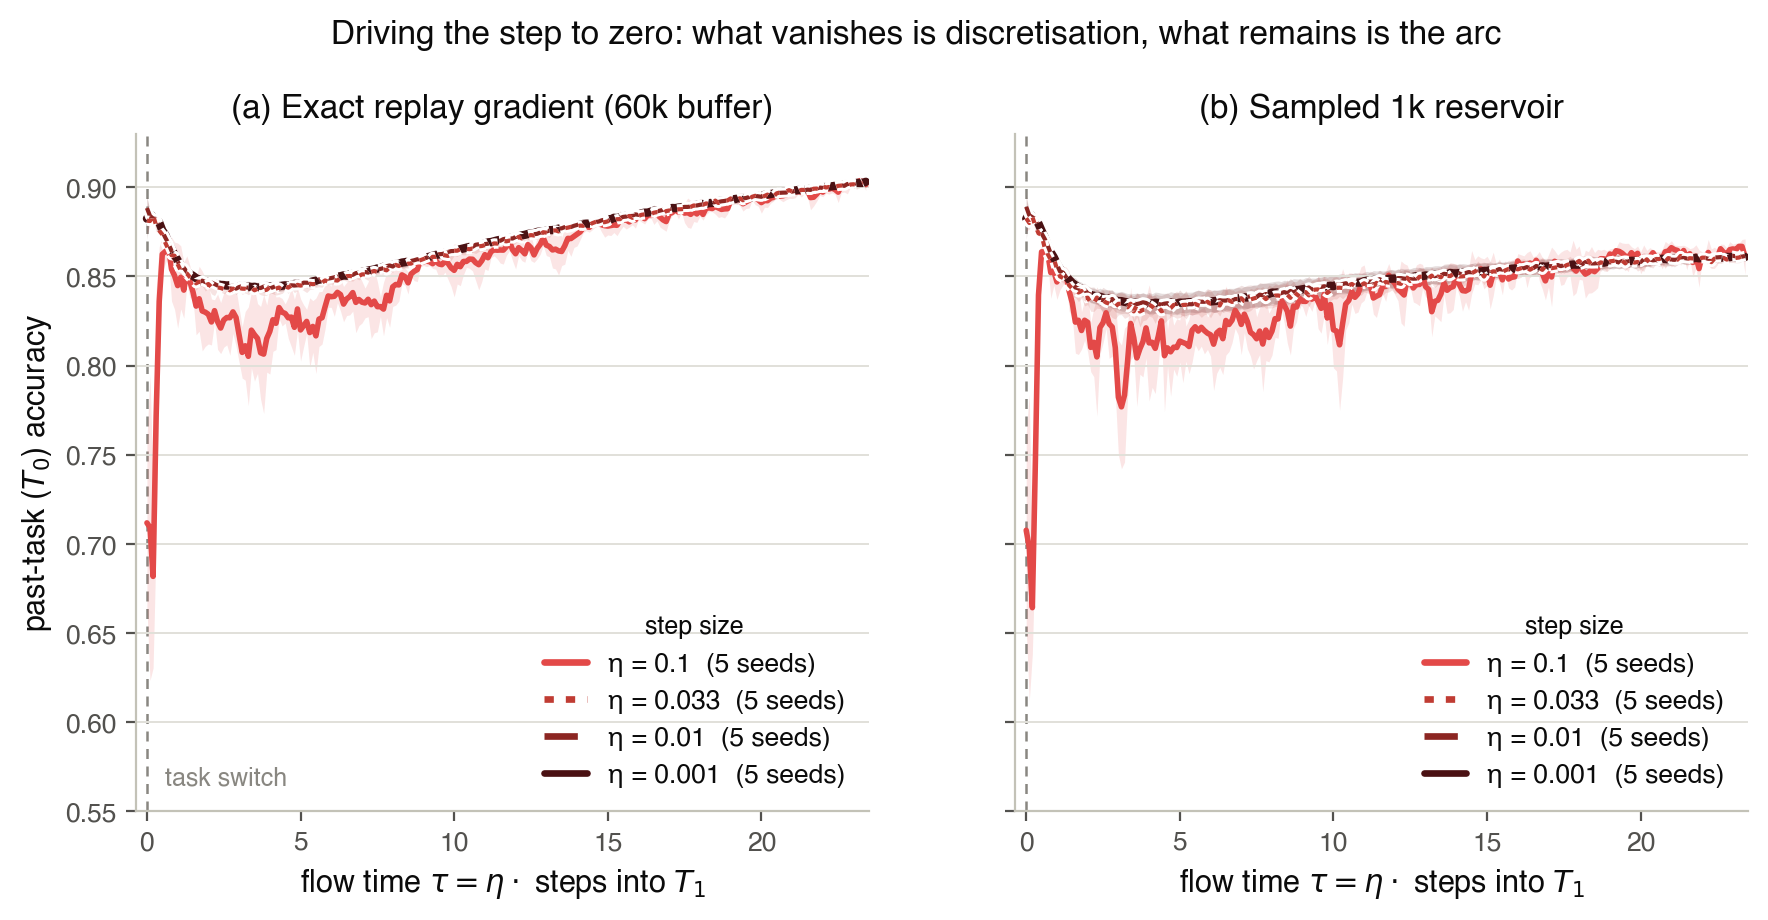
\includegraphics[width=0.86\linewidth]{img/results/ladder/step_size_ladder.png}
    \caption{The step-size ladder at momentum $0$: past-task ($T_0$) accuracy against flow time $\tau = \sum_t \eta$, seed mean with $\pm$std bands, $\tau{=}0$ the task switch. Every rung covers the same $\tau = 23.5$ from the same frozen $\theta_0^*$ and the same buffer, so within a panel $\eta$ is the only difference. (a) exact $60$k replay gradient, (b) the $1$k reservoir of the standard protocol. What the reader should see is a limit that is reached and is not zero. The standard operating point (light, $\eta = 0.1$) leaves the other three within its first two steps, drops ${\approx}20$ pp, and spends the rest of the task jittering back; the three finer rungs (dark: $\eta = 0.1/3$ and $\eta = 0.01$ dashed, $\eta = 0.001$ solid) have no boundary spike at all, and overlap so closely that linestyle rather than colour is what separates them. What they do have is a smooth dip-and-recover bend that neither the smaller step nor the exact gradient removes: the arc.}
    \label{fig:ladder}
\end{figure*}

\paragraph{The ladder converges, and not on zero.}
At momentum $0$ the three finest rungs are all but the same run. On the exact arm depth falls $22.3 \rightarrow 4.2 \rightarrow 3.9 \rightarrow 3.8$ pp for $\eta = 0.1 \rightarrow 0.1/3 \rightarrow 0.01 \rightarrow 0.001$, with the flow-time area at $0.590 \rightarrow 0.360 \rightarrow 0.346 \rightarrow 0.341$ and ACC at $0.895 \rightarrow 0.897 \rightarrow 0.897 \rightarrow 0.898$; on the sampled arm, $22.9 \rightarrow 5.6 \rightarrow 4.9 \rightarrow 4.7$ pp, area $0.577 \rightarrow 0.293 \rightarrow 0.275 \rightarrow 0.270$, ACC $0.874 \rightarrow 0.876 \rightarrow 0.877 \rightarrow 0.877$ (all sixteen cells with their full metric set in Appendix~\ref{app:ladder_full}).
The last step down each ladder, a further tenfold cut from $\eta = 0.01$ to $\eta = 0.001$, moves depth by $0.1$ and $0.2$ pp against the $18.1$ and $17.3$ pp the first step removes, and the trajectories themselves coincide: the largest separation between the $\eta = 0.1/3$ and $\eta = 0.01$ curves anywhere on the common flow-time grid is $0.007$ (exact) and $0.006$ (sampled) in accuracy, against $0.201$ and $0.219$ for $\eta = 0.1$, both attained at $\tau \approx 0.2$, inside the coarse rung's first two steps (Figure~\ref{fig:ladder}). These residual differences are small but not noise: three of the four contrasts between those two rungs are unanimous in sign across seeds ($p = 0.0625$; the exception is the sampled area, four of five, $p = 0.125$), which is what an $O(\eta)$ remainder should look like. Extrapolating $A(\eta) = A_0 + k\eta$ through the fine rungs alone puts the limit at $3.8$ pp of depth and $0.34$ of area on the exact arm, $4.7$ pp and $0.27$ on the sampled one. That positive limit is RQ1's answer: an excursion that survives both the exact gradient and the vanishing step has no Level-Two driver left to attribute it to, and it is the arc of Section~\ref{subsec:trajectory_problem} measured rather than inferred. The all-rung least-squares fit is not the estimate to read here: over a $100\times$ lever arm the line is pinned by the coarse rung, whose excess inflates the slope to $k \approx 2.0$, pulls the depth intercept down to $1.5 \pm 1.1$ pp, and leaves a largest residual of $3.8$ pp, the size of the very quantity being estimated. That is the linear model reporting that one of its four points does not belong to its regime.

\paragraph{The coarse rung sits above the line.}
How far it sits above is the sharpest single number the block produces: $17.2$ pp of depth and $0.19$ of area on the exact arm, $15.6$ pp and $0.24$ on the sampled one. This excess is by construction what the $O(\eta)$ model cannot account for, and it is the discrete instability itself, so between two thirds and three quarters of the depth measured at the standard operating point is not a property of the trajectory the optimiser is following. It is not estimator noise either: the departure on the exact arm, where the replay gradient carries no sampling error at all, is the larger of the two in depth. This is also where the ladder settles what the boundary imbalance is. The imbalance is identical at every rung, the same near-zero replay gradient meeting the same large new-task gradient at the same $\theta_0^*$, since a rescaling of $\eta$ leaves the vector field untouched; yet the spike it produces is gone by $\eta = 0.1/3$ and the excursion that remains is smooth. The imbalance is Level-One terrain, and the acute driver of the drop is the step size that meets it, exactly the division of labour Section~\ref{subsec:trajectory_problem} assigns them. The measured limit does qualify the metric mapping of that section, however: depth is overshoot-dominated at the operating point, but it is not overshoot alone, because the arc still registers $3.8$ pp of depth once the overshoot is gone.

\paragraph{Accuracy is not what the limit costs.}
Nothing on the ladder is traded away for the smaller gap. ACC is flat to slightly rising down both arms ($0.895 \rightarrow 0.898$ exact, $0.874 \rightarrow 0.877$ sampled), and min-ACC, the worst single evaluation of the run, improves sharply, $0.658 \rightarrow 0.843$ and $0.653 \rightarrow 0.834$. ($\mathrm{WP}_{100}$ falls, $0.453 \rightarrow 0.376$ and $0.454 \rightarrow 0.369$, but it is a fixed hundred-\emph{step} horizon and therefore spans a hundredth of the flow time at $\eta = 0.001$; the decline is a units artefact of the reparametrisation and is not read as a plasticity cost.) What the limit costs is compute. Matched flow time makes the epoch count scale as $1/\eta$, so the $\eta = 0.001$ rung removes $18.5$ pp of depth at a hundred times the training of the operating point, and it removes only the overshoot. This is the bar the gates of RQ2 and RQ3 have to clear: not lowering the gap, which the step size already does with no method at all, but lowering it at the standard step size and in the standard number of steps.

\paragraph{Under momentum the ladder converges too, on an arc of its own.}
Momentum multiplies the asymptotic step by $1/(1-\mu)$, so the four rungs sit at effective steps $1.0$, $0.33$, $0.1$ and $0.01$, and only the last of these reaches the range in which the $\mu = 0$ leg had settled. It does reach it. Depth falls $14.1 \rightarrow 9.9 \rightarrow 5.0 \rightarrow 2.7$ pp on the exact arm (area $0.301 \rightarrow 0.122 \rightarrow 0.061 \rightarrow 0.040$, ACC $0.965 \rightarrow 0.973$, min-ACC $0.814 \rightarrow 0.928$) and $15.4 \rightarrow 10.1 \rightarrow 5.4 \rightarrow 4.6$ pp on the sampled one (area $0.105 \rightarrow 0.021 \rightarrow 0.0034 \rightarrow 0.0006$, ACC $0.929 \rightarrow 0.942$, min-ACC $0.802 \rightarrow 0.910$). The fine-rung extrapolation puts the limit at $2.6$ pp of depth on the exact arm and $4.1$ pp on the sampled one, only $0.1$ and $0.5$ pp below the finest rung actually run, so this leg has an arc and the bottom of the ladder is close to it. What remains true of the earlier reading is narrower than it was: the coarse rung's departure is still \emph{negative} ($-10.3$ pp exact, $-6.2$ pp sampled), lying below the line through the fine rungs rather than above it as at $\mu = 0$, so the all-rung fit is still not the estimate to read. The $O(\eta)$ model breaks down at the coarse end of both legs; under momentum it breaks down by saturating rather than by exploding.

\paragraph{Momentum is not simply a longer step.}
The grid now provides two matched-effective-step diagonals, and together they say what one alone could not. At effective step $0.1$, $(\eta = 0.01, \mu = 0.9)$ against $(\eta = 0.1, \mu = 0)$ separates widely, $5.0$ pp / $0.061$ / $0.972$ against $22.3$ pp / $0.590$ / $0.895$ on the exact arm; at effective step $0.01$, $(\eta = 0.001, \mu = 0.9)$ against $(\eta = 0.01, \mu = 0)$ reads $2.7$ pp / $0.040$ / $0.973$ against $3.9$ pp / $0.346$ / $0.897$. The depth separation collapses from $17.3$ to $1.2$ pp as the matched step shrinks, which is what two legs approaching their own $\eta \rightarrow 0$ limits must do; the area separation does not, staying eightfold at the finest matched pair. What differs between the legs is therefore the shape of the residual excursion and not only its scale. This remains the secondary read Section~\ref{subsec:ladder} calls it: the legs warm-start from anchors trained at their own momentum and settle some seven accuracy points apart, so comparing their levels compares two operating points.

\paragraph{Momentum's arc is depth without tail.}
The within-leg contrast is both the safer comparison and the sharper one. On the sampled arm the momentum leg's flow-time area falls by more than two orders of magnitude across the ladder, $0.105 \rightarrow 0.0006$, and extrapolates to zero ($-0.001$), while its depth converges on $4.1$ pp. In the limit the transient that survives under momentum is a dip that recovers almost at once: it keeps the instantaneous drop and loses the hanging tail. The $\mu = 0$ arc keeps both, $4.7$ pp of depth and $0.27$ of area that no further shortening of the step removes. Of the two-part measure of Section~\ref{subsec:metrics}, then, momentum leaves essentially only the depth term standing.

\paragraph{The coarse rung reproduces the operating point in distribution.}
$\eta = 0.1$ on the sampled arm is the standard operating point, but it is not the archived vanilla-ER reference run (D1, Appendix~\ref{app:curr_full}) and is not paired with it: the ladder skips $T_0$ training so that every cell can share one $\theta_0^*$, which leaves the two protocols on different RNG streams and hence with different buffer contents seed for seed. Their distributions agree, $22.9 \pm 4.2$ against $19.5 \pm 4.1$ pp of depth and $5.77 \pm 0.80$ against $6.27 \pm 0.47$ of step-axis area, one-standard-deviation intervals overlapping on both. That is a check that warm-starting has not moved the operating point, and nothing stronger than that.

\paragraph{What the gates inherit.}
RQ1 therefore hands on a measured quantity rather than a hypothesis. At momentum $0$ the arc is $3.8$ pp of depth and $0.34$ of flow-time area at ACC $0.898$ on the exact arm ($4.7$ pp / $0.27$ / $0.877$ sampled): a residual excursion that neither the exact gradient nor any further shortening of the step reaches, because it is not a discretisation error but the path the optimiser was following all along. Removing it requires changing the path, which is what the two gates attempt, and at the standard step size, where the ladder's own remedy is not available.

\subsection{The Scalar Feedback Gate (RQ2)}
\label{subsec:res_scalar}

Table~\ref{tab:res_curriculum} reports the curriculum sweep at both momentum settings against vanilla ER. The momentum-off leg tests the schedule in isolation; the momentum-on leg is the practically relevant regime.

\begin{table*}[htbp]
    \centering
    \small
    \resizebox{\textwidth}{!}{%
        \begin{tabular}{l ccc ccc}
            \hline
                                                 & \multicolumn{3}{c}{Momentum $0.0$} & \multicolumn{3}{c}{Momentum $0.9$}                                                                                              \\
            Condition                            & \texttt{gap\_depth} (pp)           & \texttt{gap\_area\_end}            & ACC               & \texttt{gap\_depth} (pp) & \texttt{gap\_area\_end} & ACC               \\
            \hline
            Vanilla ER (baseline)                & $19.5 \pm 4.1$                     & $6.3 \pm 0.5$                      & $0.873 \pm 0.005$ & $15.9 \pm 2.6$           & $1.0 \pm 0.2$           & $0.928 \pm 0.003$ \\
            C3: Linear $N{=}200$                 & $14.3 \pm 4.6$                     & $1.8 \pm 0.6$                      & $0.828 \pm 0.025$ & $6.2 \pm 0.6$            & $0.1 \pm 0.0$           & $0.925 \pm 0.007$ \\
            C4: Adaptive                         & $12.8 \pm 2.9$                     & $2.2 \pm 0.5$                      & $0.833 \pm 0.025$ & $2.5 \pm 0.5$            & $0.3 \pm 0.1$           & $0.917 \pm 0.001$ \\
            C7: Adaptive $\lambda_{\min}{=}0.20$ & $13.9 \pm 3.4$                     & $2.7 \pm 0.6$                      & $0.837 \pm 0.031$ & $3.7 \pm 0.4$            & $0.0 \pm 0.0$           & $0.931 \pm 0.002$ \\
            \hline
        \end{tabular}%
    }
    \caption{$\lambda$-curriculum key conditions on rot-MNIST against vanilla ER, at momentum $0.0$ and $0.9$; five seeds: the longest linear ramp (C3), the pure adaptive schedule (C4), and the practical configuration (C7). The scalar feedback gate reaches a few points of depth at matched accuracy only in the momentum-on regime it is intended for. The full sweep (C1--C7), with vanilla ER's full metric row as the reference, is in Appendix~\ref{app:curr_full}.}
    \label{tab:res_curriculum}
\end{table*}

\paragraph{The schedule works as predicted, at a momentum-$0$ price.}
At momentum $0$, mean gap depth falls monotonically with the ramp length, $17.5 \rightarrow 16.2 \rightarrow 14.3$ pp at $N = 50, 100, 200$, as the $O(1/N)$ bound of Equation~\eqref{eq:bound} predicts, though successive lengths lie within the seed spread and the reduction is bought with accuracy ($0.851 \rightarrow 0.844 \rightarrow 0.828$) and a stretched tail (per-condition metrics in Appendix~\ref{app:curr_full}). The depth that remains, still in the mid-teens, is the untouched chronic driver: the schedule times the push but leaves the finite-buffer replay estimate exactly as noisy as vanilla's, so the worst evaluation keeps arriving as a late noise-driven drop, a floor no ramp length can pass and only the exact-gradient diagnostic removes (C8, Table~\ref{tab:res_c8}). The two remaining ingredients behave as designed but earn their keep only under momentum. At momentum $0$ the adaptive signal removes the knob $N$ and changes nothing else, $12.8$ pp / $2.2$ / $0.833$ against the longest linear ramp's $14.3$ pp / $1.8$ / $0.828$, with seeds split on the depth difference ($p = 0.44$); that null is specific to this momentum setting, and the momentum leg below separates the same pair unanimously in the adaptive schedule's favour. The $\lambda_{\min}$ floor is likewise inert here, $13.9$ pp / $2.7$ / $0.837$ at $\lambda_{\min}{=}0.20$ against $12.8$ pp / $2.2$ / $0.833$ without it, because early $T_1$ progress at momentum $0$ is set by the large boundary gradient the small floor cannot redirect. The momentum-$0$ curves of Figure~\ref{fig:c_curves} (dashed) show the underlying trade: a shallower past-task dip than vanilla (a), paid for in slower early $T_1$ learning (b).

\begin{figure*}[t]
    \centering
    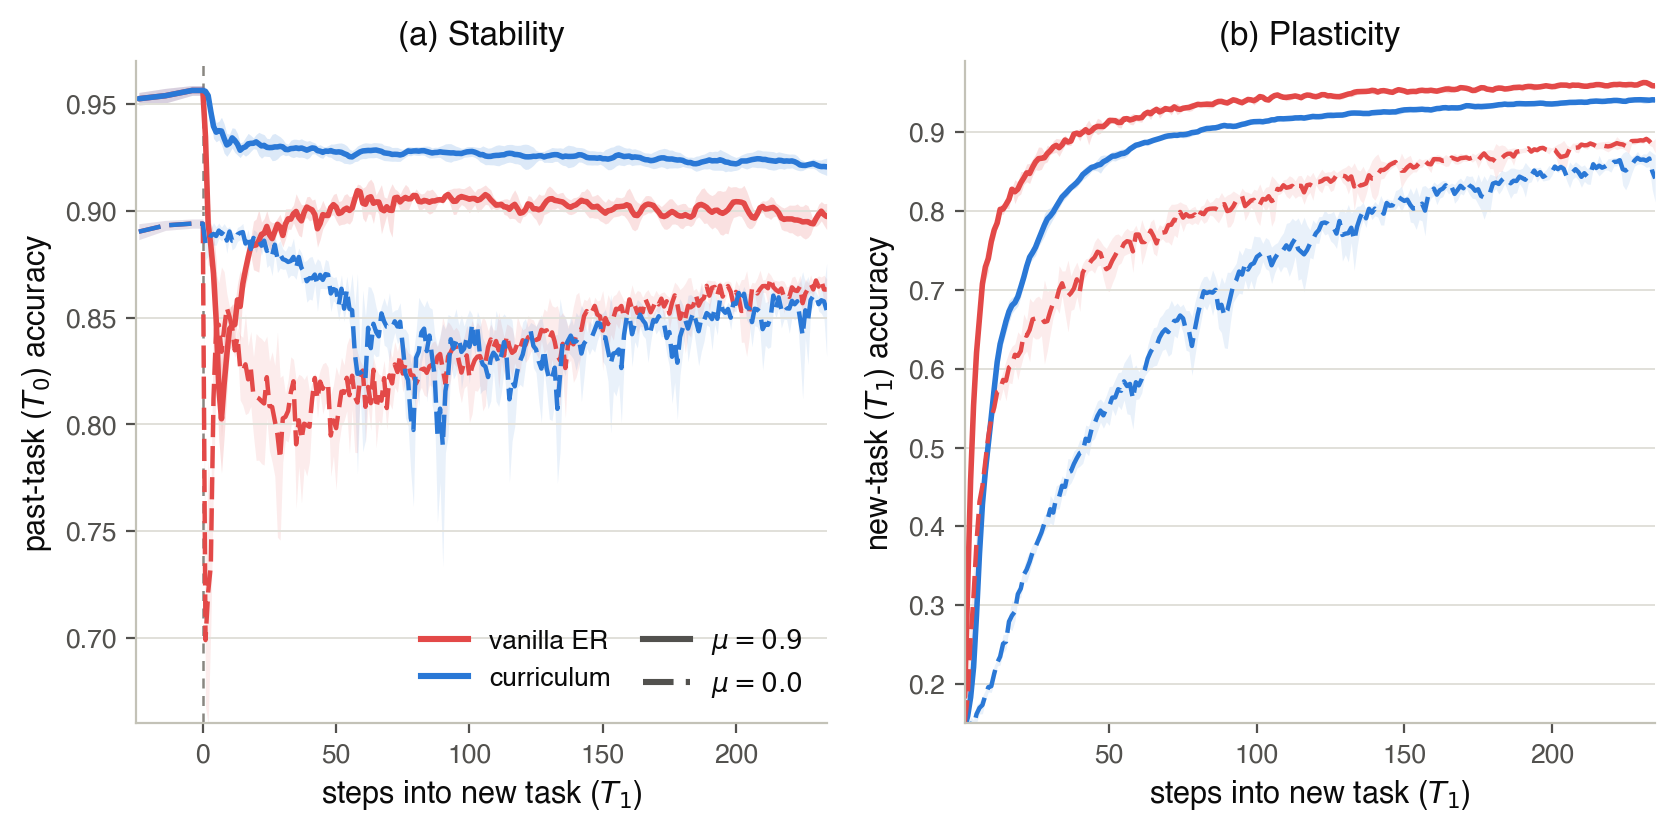
\includegraphics[width=0.85\linewidth]{img/results/curriculum/curriculum.png}
    \caption{The scalar feedback gate and momentum's two roles: per-step accuracy across the rot-MNIST switch, seed mean with $\pm$std bands, for vanilla ER (red) and the practical adaptive curriculum $\lambda_{\min}{=}0.20$ (blue), each at momentum $0.9$ (solid) and $0.0$ (dashed). \textbf{(a) Stability ($T_0$):} only curriculum-with-momentum (solid blue) holds the past task near its plateau through the switch; momentum barely dents vanilla's spike, and both methods open a deep, jittery gap without it (dashed). \textbf{(b) Plasticity ($T_1$):} at momentum $0$ the curriculum slows early new-task learning (dashed blue), the plasticity debt that momentum pays back (solid blue).}
    \label{fig:c_curves}
\end{figure*}

\paragraph{The bar is the ladder's, and at momentum $0$ the gate does not clear it.}
Lowering the gap is not by itself the gate's claim, because the step size lowers it with no method at all; the claim has to be that the gate lowers it at the standard step size and in the standard number of steps (Section~\ref{subsec:res_levels}). Nor is there an accuracy handicap to discount from the ladder's numbers: ACC is flat to rising down both arms and min-ACC improves sharply, so what the ladder charges is compute, the epoch count scaling as $1/\eta$ at matched flow time. Read against that bar on the matched $1$k arm at momentum $0$, the curriculum loses on everything but the budget. C7 leaves $13.9$ pp of depth at ACC $0.837$ and min-ACC $0.743$ in one epoch at $\eta = 0.1$; the $\eta = 0.01$ rung leaves $4.9$ pp at ACC $0.877$ and min-ACC $0.832$ in ten. Measured against its own protocol's reference the schedule removes $5.6$ pp of vanilla ER's $19.5$ and spends $3.6$ pp of ACC doing it ($0.873 \rightarrow 0.837$), where the tenfold shorter step removes $18.0$ pp of the ladder's distributionally matched $22.9$ and gains $0.3$ pp of ACC ($0.874 \rightarrow 0.877$). The flow-time areas do land together, $0.27$ for C7 against the $\eta = 0.01$ rung's $0.275$ (the curriculum's step-axis $2.7$ converted at $A_\tau = \eta A_{\text{steps}}$), but the two are referenced to plateaus four points apart and a lower plateau is a lower line to integrate against, so this is not a tie (Section~\ref{subsec:metrics}). The momentum-$0$ case for the scalar gate is therefore a case about cost and not about depth: it buys a fraction of what a shorter step buys, and buys it inside the budget a shorter step cannot keep.

\paragraph{Momentum pays the plasticity debt, and closes the gap.}
The momentum-on leg is the scalar gate's intended regime, where momentum acts through two roles at once and where both design details settle. Under momentum the adaptive signal does not merely remove the knob $N$, it outperforms the best setting of the knob it removes: $2.5$ pp / $0.3$ / $0.917$ against the tuned $N{=}200$ ramp's $6.2$ pp / $0.1$ / $0.925$, shallower in all five seeds by ${\approx}3.7$ pp, paid for in accuracy and a slightly heavier tail. The $\lambda_{\min}{=}0.20$ floor buys both back at a quantified price: $3.7$ pp / $0.03$ / $0.931$, unanimously $1.2$ pp deeper than the unfloored schedule and unanimously $1.3$ pp more accurate, with the tail an order of magnitude lighter. The two ingredients compose into a configuration that clears the tuned linear ramp on all three quantities, depth in five seeds of five and accuracy in four, and that cuts three quarters of vanilla ER's depth ($15.9$ pp / $1.0$ / $0.928$) while returning accuracy to vanilla's level. The depth collapse is variance reduction, momentum averaging the noisy replay gradient across accumulated velocity once the schedule has tempered the boundary push at source; the accuracy restoration is the separate role, acceleration, repaying the plasticity the schedule borrows.

\paragraph{C8: the pairing is forced, not found.}
Momentum is not one partner among several that happened to suit the schedule, and C8 is the step that shows why. Crossing the practical curriculum with the exact $60$k replay gradient at momentum $0$ collapses the residual the schedule leaves, $13.9 \rightarrow 0.2$ pp of depth and $2.7 \rightarrow 0.05$ of area at ACC $0.837 \rightarrow 0.818$ (Table~\ref{tab:res_c8}, Appendix~\ref{app:curr_full}). What C7 still carries at momentum $0$ is therefore estimator variance and not a second deformation of the path, so what it needs is a variance reducer rather than a second repair of the trajectory. At a $1$k memory exactly one is affordable: a $60$k buffer is the negation of the premise, while momentum averages successive replay estimates inside the velocity buffer and stores nothing to do it. C7$_M$ is in that sense the cheap substitute for C8's buffer, at $1/60$th of its memory, and the substitution runs the other way too: with the buffer exact there is no variance left for momentum to reduce, and what it still contributes shows up as accuracy alone, C8$_M$ reaching $0.955$ against C8's $0.818$ at $2.0$ against $0.2$ pp of depth. The two roles are separable, and the schedule needs one of each.

C7$_M$ ($3.7$ pp / $0.03$ / $0.931$, min-ACC $0.919$) is accordingly the configuration this thesis recommends and the one carried to CIFAR: no other limited-memory condition in the rot-MNIST study reaches a shallower gap without giving up accuracy. It is also where the gate clears the ladder's bar in its own regime. On the same $1$k arm at momentum $0.9$ the $\eta = 0.01$ rung reaches $5.4$ pp at ACC $0.940$ and min-ACC $0.901$ after ten epochs, so one epoch of the schedule is $1.7$ pp shallower and $1.8$ pp better in worst-case retention than ten epochs of a tenfold shorter step, for $0.9$ pp of ACC (the two protocols' $\eta = 0.1$ cells agree here as at momentum $0$, $15.4 \pm 2.2$ against $15.9 \pm 2.6$ pp at ACC $0.929$ against $0.928$). That rung is a rung and not a limit, but the ladder's fourth rung now supplies the limit as well, and the comparison strengthens rather than softens. At $\eta = 0.001$, a hundred epochs, the same arm reaches $4.6$ pp at ACC $0.942$ and min-ACC $0.910$, and the fine-rung extrapolation puts the $\eta \rightarrow 0$ depth of this leg at $4.1$ pp (Section~\ref{subsec:res_levels}). One epoch of the schedule is thus $0.9$ pp shallower than a hundred epochs of a hundredfold shorter step, and its $3.7 \pm 0.4$ pp sits at or below what shortening the step can ultimately reach here, for $1.1$ pp of ACC. The claim is not that the schedule beats the limit, which the seed spread does not support, but that it matches it at one hundredth of the training: what the step size buys at this momentum, it buys at a cost the schedule does not pay.

For completeness the momentum cross also confirms the vanilla-ER null: momentum shifts vanilla depth only from $19.5$ to $15.9$ pp, smaller than the seed spread with seeds split on its sign ($p = 0.44$), because the deterministic unopposed first step carries no accumulated velocity to average; it does cut vanilla's tail (area $6.3 \rightarrow 1.0$, all seeds). Momentum smooths vanilla's recovery, but it leaves the depth, the gap itself, intact.

\subsection{The Directional Feedforward Gate (RQ3)}
\label{subsec:res_directional}

RQ3 asks whether asymmetric PER shrinks the gap as its filter strengthens ($\delta \to 0$), at what plasticity cost, and where a feedforward gate fails. Table~\ref{tab:res_per} reports the $\delta$ sweep on both buffer legs at momentum $0$; the full metric set at both momentum settings is in Appendix~\ref{app:per_full}. The standard $1$k leg is the gate's practical configuration; the full-buffer leg plays the same diagnostic role as C8, switching the estimator variance off at source so that what remains of the excursion is the arc together with whatever the standard step still overshoots of it, and it does not enter the head-to-head comparisons. Both legs run at $\eta = 0.1$, so their areas are on the step axis; the ladder's flow-time arc converts to the same axis as $A_{\text{steps}} = A_\tau/\eta$.

\begin{table*}[htbp]
    \centering
    \small
    \begin{tabular}{l cccc c cccc}
        \hline
                 & \multicolumn{4}{c}{Standard (1k) buffer} &       & \multicolumn{4}{c}{Full ($60$k) buffer}                                                                               \\
        \cline{2-5}\cline{7-10}
        $\delta$ & depth (pp)                               & area  & ACC                                     & $\mathrm{WP}_{100}$ &  & depth (pp)             & area  & ACC     & min-ACC \\
        \hline
        no gate  & $19.5 \pm 4.1$                           & $6.3$ & $0.873$                                 & $0.736$             &  & $22.3 \pm 5.0^{\dagger}$ & $5.9$ & $0.895$ & $0.658$ \\
        \hline
        $1.0$    & $9.0 \pm 0.6$                            & $3.3$ & $0.869$                                 & $0.733$             &  & $4.0 \pm 1.0$          & $2.3$ & $0.898$ & $0.841$ \\
        $0.3$    & $7.4 \pm 1.1$                            & $2.3$ & $0.873$                                 & $0.736$             &  & $1.5 \pm 1.1$          & $1.0$ & $0.900$ & $0.867$ \\
        $0.1$    & $5.9 \pm 1.5$                            & $1.6$ & $0.876$                                 & $0.739$             &  & $2.2 \pm 1.6$          & $0.4$ & $0.901$ & $0.860$ \\
        $0.03$   & $4.8 \pm 1.9$                            & $1.0$ & $0.880$                                 & $0.741$             &  & $9.5 \pm 8.2$          & $0.4$ & $0.903$ & $0.787$ \\
        \hline
    \end{tabular}
    \caption{Asymmetric-PER $\delta$ sweep on rot-MNIST at momentum $0$, five seeds, against the ungated reference. Depth and area fall as $\delta \to 0$ while ACC and $\mathrm{WP}_{100}$ \emph{rise}: the directional gate protects the past task at no measured plasticity cost. On the full buffer, the diagnostic leg on which the residual excursion is the arc and the step's overshoot of it, the area falls to $0.4$ at $\delta{=}0.1$, below the $3.4$ the ladder's arc alone reads on this step axis ($A_\tau = 0.34$, Section~\ref{subsec:res_levels}). The far cell is the exception: at $\delta{=}0.03$ full buffer the mean depth jumps to $9.5$ pp with a large std, the cliffs of the text. Areas are on the step axis ($\eta = 0.1$). $^{\dagger}$The full-buffer reference is the ungated exact-gradient rung of the ladder at the same step size (S1, exact arm, $\mu{=}0$; Appendix~\ref{app:ladder_full}); it warm-starts from a frozen $\theta_0^*$ and so is not seed-paired with the sweep.}
    \label{tab:res_per}
\end{table*}

\begin{figure*}[t]
    \centering
    
\includegraphics[width=0.85\linewidth]{img/results/asymmetric_per/per_sweep.png}
    \caption{The directional feedforward gate: per-step past-task ($T_0$) accuracy across the rot-MNIST switch at momentum $0$, sweeping the damping $\delta$ (weaker filter light $\rightarrow$ stronger filter dark). \textbf{(a) Standard $1$k buffer:} the boundary dip shrinks monotonically as $\delta \to 0$, and accuracy rises with it (Table~\ref{tab:res_per}), so the protection is bought at no plasticity cost. \textbf{(b) Full $60$k buffer} (variance driver off, so the residual excursion is the deterministic arc together with the standard step's overshoot of it): the excursion shrinks with the filter for $\delta \ge 0.1$, but at the strongest setting $\delta{=}0.03$ the gate fails late and abruptly: shown per seed (critical red), $3$ of $5$ seeds hold flat for ${\sim}200$ steps and then slide off a late cliff, a failure mode a feedback signal does not share.}
    \label{fig:per_curves}
\end{figure*}

\paragraph{Monotone, at no measured plasticity cost.}
On the standard buffer, depth falls from $9.0$ to $4.8$ pp as $\delta$ goes from $1.0$ to $0.03$ while ACC \emph{rises} from $0.869$ to $0.880$ and $\mathrm{WP}_{100}$ from $0.733$ to $0.741$; every one of these trends holds across all five seeds (Figure~\ref{fig:per_curves}(a)). To be precise about what is claimed: the filter does slow the new task, but selectively, only along the directions the past-task curvature flags, never by scaling the whole loss down as the scalar gate does. The new-task learning curves show the honest version of this claim (Figure~\ref{fig:per_plasticity}): at the strongest filter the $T_1$ curve is visibly slower over roughly the first fifty steps, the expected signature of the selective slowdown, and indistinguishable from vanilla ER thereafter; by the $\mathrm{WP}_{100}$ horizon no cost remains, and the roughly $4$ pp of accuracy the scalar gate pays at momentum $0$ never materialises here. This is the scalar gate's weakness inverted, and it is what makes the two gates complements. The full-buffer leg turns the filter on the arc: with the variance driver off, the area shrinks with the filter, $2.3 \rightarrow 1.0 \rightarrow 0.4$ for $\delta = 1.0 \rightarrow 0.3 \rightarrow 0.1$ (the $1.0 \rightarrow 0.3$ drop holds across all seeds) at ACC $0.898 \rightarrow 0.900 \rightarrow 0.901$, so the directional gate bends the followed path back toward the reference, as the curriculum does by another route. The contrast that makes the mechanism point is with the ladder. On the same exact gradient, shortening the step converges on $0.34$ of flow-time area, $3.4$ on the step axis these runs are measured on, and going below that is what no smaller step achieves; the ungated exact-gradient run at this step size reads $5.9$ there, and the gate at $\delta{=}0.1$ takes it to $0.4$ without touching the step size at all. The gate reaches the arc itself, which no repair of the step does. This is a mechanism reading rather than an operating point, since the full buffer that isolates the arc defeats the limited-memory premise. Leaving the restoring gradient $g_{\text{rep}}$ at full strength is what makes this a net removal of damage rather than a reshuffling of it: a symmetric variant that preconditions the summed update strangles the restoring gradient harder than the harmful push, so its forgetting \emph{climbs} as the filter strengthens (Appendix~\ref{app:per_sym}, Table~\ref{tab:res_per_sym}).

\begin{figure*}[t]
    \centering
    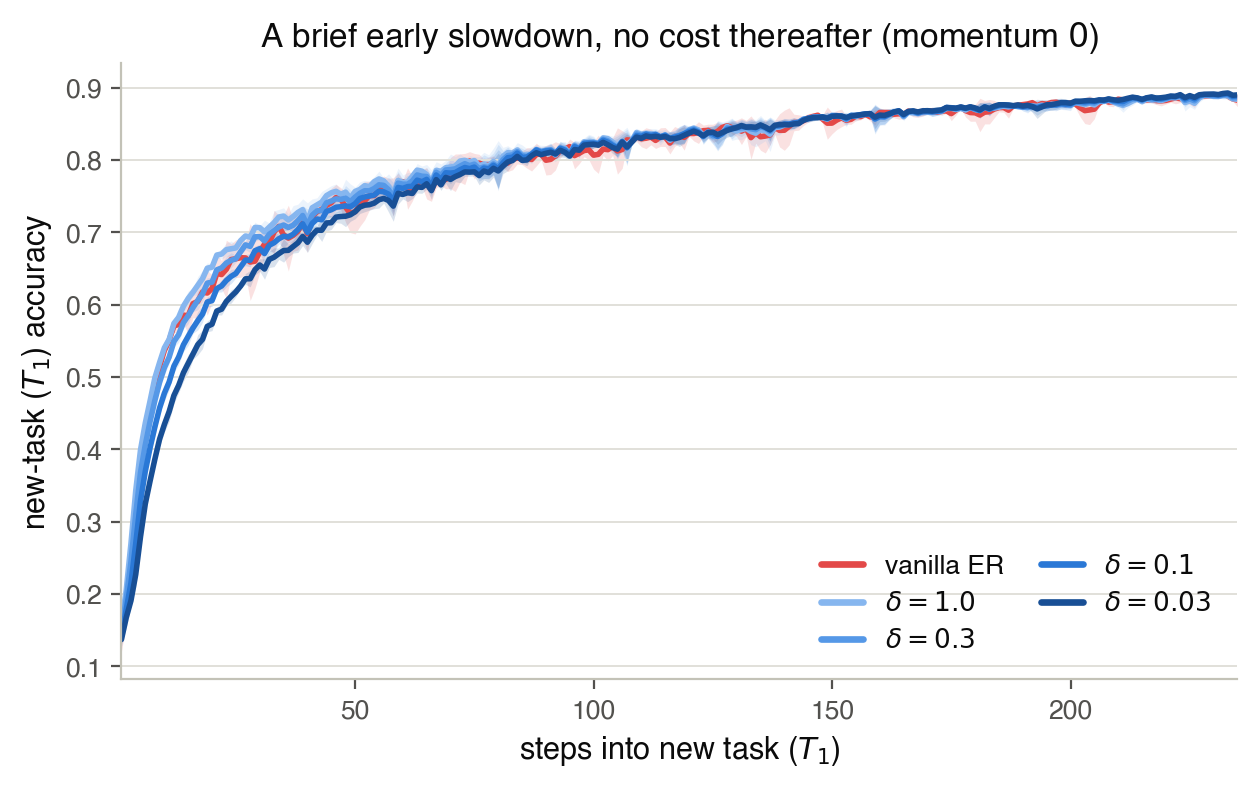
\includegraphics[width=0.8\linewidth]{img/results/asymmetric_per/per_plasticity.png}
    \caption{New-task ($T_1$) accuracy across the rot-MNIST switch at momentum $0$ for the standard-buffer $\delta$ sweep against vanilla ER (red); seed mean with $\pm$std bands. The strongest filter ($\delta{=}0.03$, darkest) lags briefly over the first ${\approx}50$ steps, the selective slowdown along past-task-sharp directions, and matches vanilla from then on; the plasticity metrics at horizon $100$ and beyond record no cost (Table~\ref{tab:res_per}).}
    \label{fig:per_plasticity}
\end{figure*}

\paragraph{The cliffs: an unexpected late failure.}
The one place the sweep breaks monotonicity is the strongest full-buffer setting, $\delta = 0.03$, where mean depth jumps to $9.5$ pp with a std of $8.2$: in $3$ of $5$ seeds the past-task curve holds flat for roughly two hundred steps and then slides off a late cliff, the red per-seed traces in Figure~\ref{fig:per_curves}(b). A solver control rules out the most straightforward explanation: rerunning the setting with the conjugate-gradient solver at $60$ iterations instead of $25$ reproduces the cliffs at the same seeds and steps ($11.5$ pp mean depth), so they are not an artefact of an under-converged solve. The cliffs came as a surprise: the account made no prediction of a late, abrupt failure, and nothing in the rest of the sweep hints at one. They are also confined to the exact-gradient diagnostic: at the same $\delta$ on the standard $1$k buffer no seed shows one (depth $4.8 \pm 1.9$ pp, the monotone end of the sweep). The failure is tied to the exact replay gradient: the sampling jitter of a practical buffer appears to protect against it, the same noise that elsewhere drives the overshoot here keeping the iterate from settling into the escape direction. Why the cliffs happen we can only partly say. A reading consistent with the data is a blind spot of the gate's model of the past task: the filter passes new-task pressure through directions its sampled Fisher rates as flat, and in these seeds that trust appears to be misplaced further out along the trajectory. We offer this as a hypothesis, not an established mechanism. What the control does establish is that the strongest filter can fail late and abruptly when nothing perturbs it. Because the failure is confined to the diagnostic leg, it is unlikely in a practical configuration, but it exposes a real weakness of feedforward control.

\paragraph{Momentum re-inflates the per-step filter.}
Momentum undoes the directional gate's protection, the opposite of what it does for the scalar gate, and it does so on both legs: on the practical $1$k buffer depth climbs from $4.8$ to $8.5$ pp at $\delta{=}0.03$ (Figure~\ref{fig:regime}), and on the full-buffer diagnostic from $2.2$ to $7.6$ pp at $\delta{=}0.1$ and from $1.5$ to $9.1$ pp at $\delta{=}0.3$ (both across all five seeds). Momentum accumulates the already-filtered direction, but the filter attenuates the step, not the source: the new-task loss, and with it the per-step gradient, keeps its full size, and because motion in the braked directions is slow, the shrunk push persists there step after step. A persistent push entering the accumulator is amplified toward $1/(1-\mu)$ times its per-step size, so velocity rebuilds displacement in the very directions the filter shrinks one step at a time. This re-inflation is what makes the head-to-head comparison of the next subsection regime-dependent.

\subsection{Reading the Momentum Crosses Together}
\label{subsec:res_regimeflip}

Read side by side in both gates' practical regime, the $1$k reservoir, the curriculum's and the directional gate's momentum crosses show that the two gates do not sit on a fixed stability--plasticity frontier a practitioner trades along: which gate leaves the smaller gap is decided by the momentum setting, the same setting that decides final accuracy. Figure~\ref{fig:regime} shows it directly, the same three methods at the same buffer with only the momentum setting changed between the panels.

\begin{figure*}[t]
    \centering
    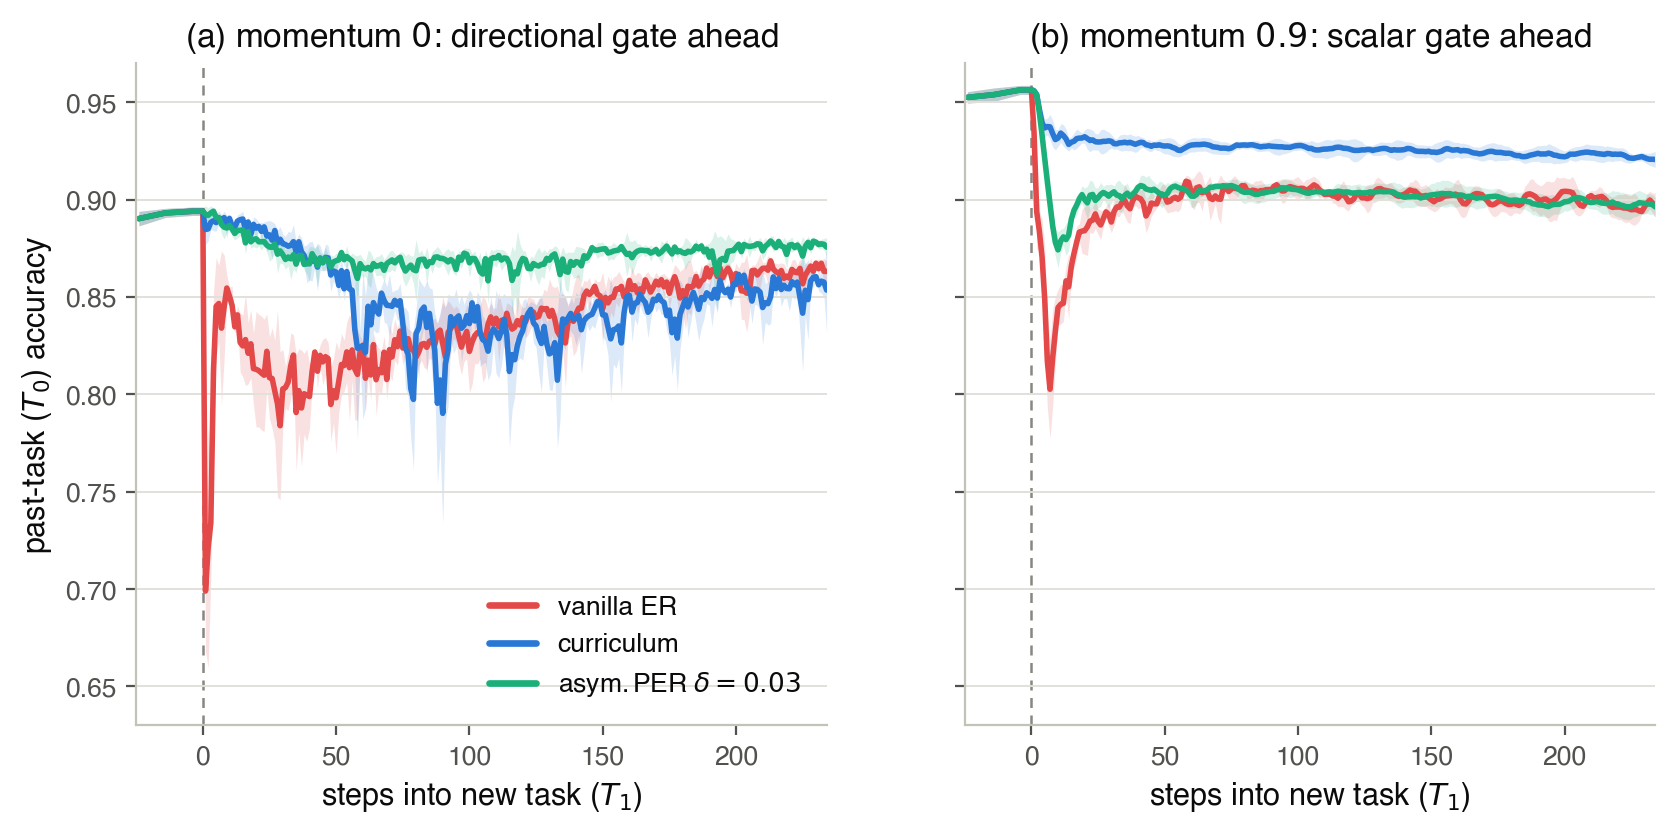
\includegraphics[width=0.85\linewidth]{img/results/momentum/regime_flip.png}
    \caption{The momentum synthesis at the matched $1$k buffer: per-step past-task ($T_0$) accuracy across the rot-MNIST switch for vanilla ER (red), the practical curriculum C7 (blue), and asymmetric PER at its strongest standard-buffer filter $\delta{=}0.03$ (aqua); seed mean with $\pm$std bands, $x{=}0$ the task switch. \textbf{(a) Momentum $0$:} the directional gate holds $T_0$ highest ($4.8$ pp / ACC $0.880$) while the curriculum opens a deep, noisy dip ($13.9$ pp / $0.837$). \textbf{(b) Momentum $0.9$:} the ordering swaps: the curriculum holds $T_0$ near its plateau ($3.7$ pp / $0.931$) while accumulated velocity re-inflates the directional gate's per-step filter ($8.5$ pp / $0.929$). The pre-switch level is higher in (b) because momentum converges $T_0$ higher before the switch.}
    \label{fig:regime}
\end{figure*}

At momentum $0$ the directional gate is better on both axes: $4.8$ pp of depth at $0.880$ accuracy against the curriculum's $13.9$ pp at $0.837$, with no measured plasticity debt to leave unpaid, and its one remaining cost is the per-step conjugate-gradient solve against the scalar gate's single gradient-norm ratio (Table~\ref{tab:res_cost}). Momentum, standard on realistic backbones and decisive for final accuracy at these budgets, reverses the ranking through the re-inflation mechanism above: the directional gate climbs to $8.5$ pp at the matched buffer while the curriculum, attenuating at source, reaches $3.7$ pp at vanilla accuracy, and with the buffers matched the directional gate has no accuracy advantage left to offset its re-inflated gap ($0.929$ vs.\ $0.931$). The choice between the gates is therefore not a point on a frontier but a consequence of whether momentum is on: off, take the directional gate; on, take the scalar gate. A five-task rot-MNIST sequence reproduces this picture across four consecutive boundaries: at momentum $0$ the directional gate keeps its edge, under momentum the curriculum keeps the least cumulative forgetting while the re-inflated directional gate falls back to vanilla ER's level (Appendix~\ref{app:longseq_full}, Figure~\ref{fig:longseq}).

\subsection{Generalisation to CIFAR-10 (RQ4)}
\label{subsec:res_cifar}

The CIFAR-10 block tests whether both gates carry to a ResNet-18, a clean $\rightarrow$ corruption shift, and the two normalisations that govern the post-switch recovery. Table~\ref{tab:res_cifar} reports the headline block at momentum $0.9$, the practically relevant regime.

\begin{table*}[htbp]
    \centering
    \small
    \begin{tabular}{ll cccc}
        \hline
        Norm & Method                                   & \texttt{gap\_depth} (pp) & \texttt{gap\_area\_end} & ACC               & min-ACC           \\
        \hline
        \multirow{3}{*}{BatchNorm}
             & G1: Vanilla ER                           & $11.8 \pm 2.5$           & $17.5 \pm 4.6$          & $0.723 \pm 0.008$ & $0.644 \pm 0.023$ \\
             & G2: Curriculum ($\lambda_{\min}{=}0.20$) & $\mathbf{4.8 \pm 0.7}$   & $\mathbf{3.6 \pm 2.2}$  & $0.722 \pm 0.011$ & $0.713 \pm 0.017$ \\
             & G3: Asym.\ PER ($\delta{=}0.1$)          & $5.9 \pm 4.3$            & $3.3 \pm 3.0$           & $0.715 \pm 0.011$ & $0.698 \pm 0.023$ \\
        \hline
        \multirow{3}{*}{GroupNorm}
             & G4: Vanilla ER                           & $41.2 \pm 13.5$          & $34.9 \pm 23.7$         & $0.730 \pm 0.011$ & $0.309 \pm 0.111$ \\
             & G5: Curriculum ($\lambda_{\min}{=}0.20$) & $\mathbf{5.2 \pm 2.1}$   & $\mathbf{1.7 \pm 0.9}$  & $0.731 \pm 0.020$ & $0.670 \pm 0.055$ \\
             & G6: Asym.\ PER ($\delta{=}0.1$)          & $5.6 \pm 1.1$            & $4.8 \pm 3.8$           & $0.741 \pm 0.009$ & $0.673 \pm 0.023$ \\
        \hline
    \end{tabular}
    \caption{CIFAR-10 headline block (ResNet-18, momentum $0.9$, buffer $5{,}000$, five seeds). Both gates cut gap depth and area far below vanilla ER at matched final accuracy and much higher worst-case retention (min-ACC), under both normalisations. Neither was given a CIFAR-specific sweep; both carry their rot-MNIST configurations.}
    \label{tab:res_cifar}
\end{table*}

\paragraph{Both gates carry to the deeper backbone.}
The rot-MNIST result carries over and strengthens. Under batch norm the curriculum cuts depth from $11.8$ to $4.8$ pp and asymmetric PER to $5.9$ pp; under group norm, where vanilla ER suffers a catastrophic $41.2$ pp drop, the curriculum cuts it to $5.2$ pp and asymmetric PER to $5.6$ pp. Every gate-vs-vanilla depth and area contrast holds across all five seeds, at final accuracy within about $0.01$ of vanilla and with worst-case retention sharply improved, min-ACC rising from $0.31$ to $0.67$ under group norm. On this backbone the transient stays open for hundreds of steps, so the area carries as much of the comparison as the depth (Figure~\ref{fig:cifar_curves}): vanilla ER under group norm crashes $T_0$ almost to chance and crawls back over the whole recovery window, while both gates hold $T_0$ near its plateau through the switch. At the matched $5{,}000$ buffer and momentum $0.9$ both gates land in the same few-pp band, with the curriculum the cheaper of the two (below), consistent with the momentum regime of Section~\ref{subsec:res_regimeflip}. The few-pp dip both gates keep under batch norm is boundary-localised and recovers within tens of steps, consistent with the running statistics re-adapting to the shifted inputs, a pathway no gate on the update touches (Appendix~\ref{app:cifar_headline_full}).

\begin{figure*}[t]
    \centering
    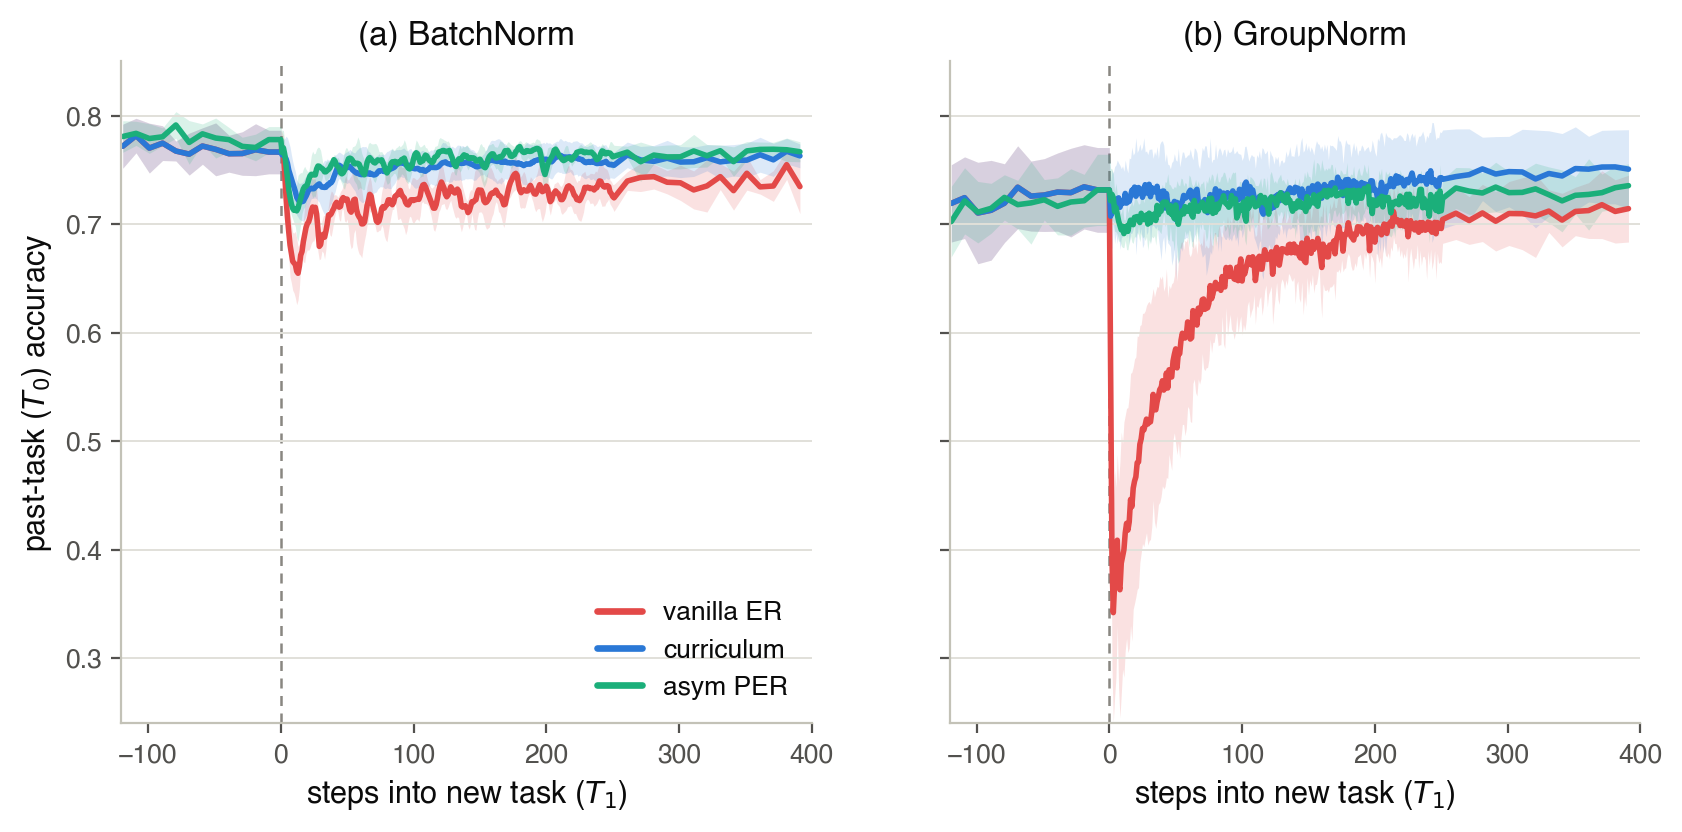
\includegraphics[width=0.85\linewidth]{img/results/cifar/cifar_headline.png}
    \caption{Per-step past-task ($T_0$) accuracy across the CIFAR-10 transition (ResNet-18, momentum $0.9$, buffer $5{,}000$), one panel per normalisation, each overlaying vanilla ER (red), the practical curriculum (blue) and asymmetric PER (aqua); seed mean with $\pm$std bands, $x{=}0$ the task switch. \textbf{(a) BatchNorm:} vanilla ER dips and re-adapts slowly while both gates hold $T_0$ near its plateau. \textbf{(b) GroupNorm:} vanilla ER's transient is deep and long, whereas both gates hold $T_0$ flat through the switch (Table~\ref{tab:res_cifar}, Appendix~\ref{app:cifar_headline_full}).}
    \label{fig:cifar_curves}
\end{figure*}

\paragraph{Mechanism, generalisation, and cost.}
Three further checks are reported in full in Appendix~\ref{app:cifar_extra}. A momentum cross on the deep backbone (Table~\ref{tab:res_cifar_mom}) turns out to be only weakly informative: at momentum $0$ the ResNet under-converges in ten epochs (vanilla ACC $0.65$, against $0.730$ with momentum), and on that degraded baseline both gates improve with momentum by similar margins ($28.6 \rightarrow 5.2$ pp for the curriculum, $22.6 \rightarrow 5.6$ pp for the directional gate), so the cross cannot separate the predicted composition from a general convergence gain; the vanilla depth null ($40.5 \rightarrow 41.2$ pp) sits on the same degraded baseline. The momentum signatures therefore rest on the rot-MNIST results, where the MLP isolates them cleanly (Section~\ref{subsec:disc_limits}). A generalisation block (Appendix~\ref{app:cifar_gen_full}, Table~\ref{tab:app_cifar_gen}) shows the curriculum beating a paired vanilla control on two corruptions it was never tuned on (shot noise $46.3 \rightarrow 7.3$ pp, contrast $8.4 \rightarrow 3.9$ pp under group norm), with a single three-task group-norm sequence flagged as a reliability boundary of the adaptive ratio when two consecutive corruptions are near-identical and both gradient norms become small (Figure~\ref{fig:failure_curves}; traced in Appendix~\ref{app:cifar_gen_full}). Finally, compute separates the gates where retention does not (Table~\ref{tab:res_cost}): the scalar gate is one gradient-norm ratio on top of a standard ER step and leaves the GPU half-idle, while the directional gate's $25$ conjugate-gradient Fisher-vector products per step saturate it, costing ${\sim}16\times$ the wall-clock and ${\sim}24\times$ the GPU energy on the ResNet-18 at similar peak memory; on the MLP both runs finish in under half a minute and the difference is negligible. In the momentum regime standard in practice, then, the scalar gate matches the directional gate's retention at essentially vanilla-ER cost and without the blind-spot cliffs, which is why it is the default recommendation.

\subsection{Summary of Findings}
\label{subsec:res_summary}

The account holds end to end, with one revision it forced. The gap separates into overshoot of the followed path and a deterministic arc of the intended one (RQ1), and the step-size ladder separates them as a limit: at momentum $0$ the excursion falls as $\eta \rightarrow 0$ but not to zero, converging on $3.8$ pp of depth and $0.34$ of flow-time area at ACC $0.898$ on the exact replay gradient ($4.7$ pp / $0.27$ / $0.877$ on the sampled buffer), so between two thirds and three quarters of the depth measured at the standard operating point is discretisation overshoot and the remainder is the path itself. That remainder is the revision the measurement forced on the account's metric mapping: depth is overshoot-dominated at the operating point but it is not overshoot alone. The arc is what the gates have to remove, and at the standard step size, where the ladder's own remedy costs a hundredfold longer run. The scalar feedback gate with momentum reaches $3.7$ pp of depth at vanilla accuracy, and C8 shows the pairing to be forced rather than fortunate, since the residual the schedule leaves at momentum $0$ is estimator variance and momentum is the variance reducer a $1$k memory can afford (RQ2); the directional feedforward gate shrinks depth and arc monotonically at no measured plasticity cost, but fails late and abruptly at its strongest diagnostic setting and re-inflates under momentum (RQ3); the comparison is therefore regime-dependent, and both gates carry to CIFAR-10 at matched accuracy and much improved worst-case retention (RQ4). The discussion reads these findings against the account of Section~\ref{sec:motivation}.

\section{Discussion}
\label{sec:discussion}

The results support the two-level account and, with it, the gate view of replay. This section reads them back against the theory, weighs the limits of the evidence, and draws out what follows for method design.

\subsection{Why the gap needs two levels}
\label{subsec:disc_twolevel}

The central empirical claim is that the stability gap is not one quantity but two failures of the same optimisation, kept apart because they answer to different interventions, and the $2\times2$ of Section~\ref{subsec:res_levels} is the direct test: removing the overshoot drivers leaves the arc, fixing the path leaves the overshoot, and only doing both closes the gap. Neither intervention is a weaker version of the other. The arc is a property of which path the descent dynamics define, and no amount of optimiser hygiene (exact gradients, balanced magnitudes, zero noise) touches it; the overshoot is how far the discrete, noisy, accelerated iterate leaves whatever path it is on, and no change of path removes it. An intervention aimed at one level is silent on the other.

The natural alternative, a single additive decomposition of the gap into magnitude, variance, and trajectory shares, does not survive the data: the shares are order-dependent (a noisy replay gradient inflates the first-step magnitude), and the mapping from factors to metrics is crossed by the experiments, the curriculum's momentum-$0$ tail looking like a ``trajectory'' term until C8 removes it with the exact buffer and no momentum at all, revealing it as variance (Table~\ref{tab:res_c8}). The two-level split is instead by kind: which path is followed versus how tightly it is followed.

The split also settles what the gap is not the price of: C8 closes the transient to $0.2$ pp while its accuracy sits $5.5$ pp below vanilla ER (Section~\ref{subsec:res_levels}), so the permanent rise to the joint-basin level is the stability--plasticity cost and everything below the settled level and back is failure to follow the monotone reference path, not the cost of learning. This is why the end-referenced area is anchored to the recovered plateau rather than the pre-switch baseline: it attributes the gap to the trajectory rather than to capacity loss.

Finally, the two levels explain why the metric that matters changes with the backbone. On the MLP the network reconverges in a few steps, so the arc integrates to little and the perceived severity is the overshoot spike; on the ResNet the same transient stays open for hundreds of steps (Figure~\ref{fig:cifar_curves}), so the slow tail is where most of the lost accuracy accumulates and where both gates' margin over vanilla is largest (Table~\ref{tab:res_cifar}). Depth and area are the signatures of the two levels, and a depth-only reading would have understated the result on exactly the architectures where continual-evaluation cost is highest.

\subsection{Two gates, two ways to divide the work}
\label{subsec:disc_gates}

Written in the unified update of Section~\ref{subsec:gates}, every replay method gates the new-task push while restoring at full strength, and the curriculum and asymmetric PER are the two pure corners of the taxonomy: a scalar gate driven by feedback, and a directional gate driven by feedforward. The results show the two corners working and failing exactly where the taxonomy says they should, and the single fact that organises the whole comparison is \emph{where} the gate attenuates the push.

The scalar feedback gate attenuates at source: it multiplies the entire new-task loss by a schedule that starts near zero, so early in the transition there is almost no push to discretise, accumulate, or let noise act on. Three consequences follow, and the data confirm each. It composes with momentum, because the accumulator never sees a sustained full-strength push to rebuild (Section~\ref{subsec:res_scalar}). It has no curvature blind spot, because the adaptive schedule reads a live damage signal rather than a model of the past task. And it pays a plasticity debt: holding the loss down slows the new task, which is why C8 at momentum $0$ is gap-free but $5.5$ pp down on accuracy, a debt only acceleration repays (momentum lifts C8 from $0.818$ to $0.955$, Table~\ref{tab:res_c8}). The scalar gate's price is plasticity, and momentum is how it is paid.

The directional feedforward gate attenuates per step: it filters the push through the replay Fisher, never slows the new task at source, and so protects the past task at no plasticity cost, ACC and short-horizon plasticity rising as the filter strengthens (Table~\ref{tab:res_per}). The same per-step locality is its weakness on two axes, one the taxonomy predicts and one that emerged unanticipated. Under momentum the protection unravels by the re-inflation mechanism of Section~\ref{subsec:res_directional}, depth climbing from ${\approx}2$ to ${\approx}8$ pp: the same lever that closes the scalar gate's gap re-opens the directional gate's, and the difference is entirely where the attenuation is applied, at the source or at the step. That one distinction accounts for the whole momentum column of the study: the vanilla null, the curriculum's composition, and the directional gate's re-inflation.

The directional gate's second failure was not predicted, and it is the sharper one because it makes the case for feedback. At the strongest filter the past-task curve can slide off a late cliff (the $\delta{=}0.03$ full-buffer cliffs of Section~\ref{subsec:res_directional}). A plausible reading is a blind spot of its curvature model: the sampled Fisher rates a direction flat that the true past-task loss punishes further out, and new-task pressure escapes through it. The exposure is characteristic of feedforward control, whose gate can only be as good as its model of the past task; a feedback gate instead reads the damage as it arrives, and its own weakness lies in the conditioning of the signal it reads, as the three-task sequence shows (Section~\ref{subsec:disc_limits}). The cliffs and the plasticity debt are thus the two gates' defining and complementary costs, the feedforward gate cheap in plasticity but myopic, the feedback gate harder to blindside but slow, and this is why the two flip with momentum rather than sitting on a fixed frontier (Section~\ref{subsec:res_regimeflip}). Both gates carry to the ResNet at matched accuracy and much improved worst-case retention (Table~\ref{tab:res_cifar}), though the momentum cross there is confounded (Section~\ref{subsec:disc_limits}); it is the gate principle, not either particular method, that generalises.

\subsection{What the account changes in the literature}
\label{subsec:disc_literature}

The two-level split settles what reads as a disagreement between the two accounts of the gap that Section~\ref{subsec:stability_gap} set out. \citet{delange2023continualevaluationlifelonglearning} trace the drop to the gradient imbalance at the boundary; \citet{hess2024complementaryperspectivescontinuallearning} show the gap survives training on the exact joint loss, and \citet{kao2021naturalcontinuallearningsuccess} derive the geometry that makes it do so. Each account is right about one level and silent on the other. The imbalance is the acute driver of the overshoot: balancing it away is by far the largest single lever on depth in the driver ladder ($19.5 \rightarrow 5.7$ pp), and it leaves the arc untouched. The persistence under exact gradients is the arc: D4 reproduces it under exact, balanced, noiseless replay and measures what remains, $1.9$ pp of depth and an area of $3.2$, a controlled counterpart of the joint-loss observation and a quantification of the analytical mechanism. Read this way the two accounts stop competing. Most of the measured depth is the overshoot the imbalance account describes; most of what no repair of the update can remove is the geometry the trajectory account describes; and a mitigation aimed at either alone leaves the other level standing, which is the practical content of the $2\times2$.

The unified update of \citet{sodhani2022introductionlifelongsupervisedlearning} sorts replay methods by which weight they move and from what signal; the results add the axis that turned out to be decisive, where the modulation is applied. A-GEM and MEGA hold the new-task weight at one and correct per step from a live signal \citep{chaudhry2019efficientlifelonglearningagem, guo2020improvedschemesepisodicmemorybased}, which places them on the step side of the source/step divide, the side whose protection momentum unwinds in Section~\ref{subsec:res_directional}. The account therefore predicts that their boundary protection weakens under momentum as the directional gate's does, while source-attenuating schedules compose with it. These results do not test that prediction, but it is directly testable, and it matters because the original comparisons predate the continual-evaluation lens: end-of-task metrics would not have registered per-step protection eroding, any more than they register the gap itself.

Mode connectivity enters the account as an existence result and exits as a control result. \citet{garipov2018losssurfacesmodeconnectivity} and, for the continual setting, \citet{mirzadeh2020linearmodeconnectivitymultitask} establish post hoc that the relevant solutions share a low-loss corridor; the corridor is inspected after training and says nothing about whether an optimiser can be kept inside it while learning. C8 supplies the dynamic counterpart: an update rule whose iterate tracks the monotone reference path through the transition ($0.2$ pp of depth), turning the observation that a benign route exists into the statement that a gate can make training follow it. The same experiment sharpens the stability--plasticity dilemma \citep{Mermillod2013Stability-Plasticity} into a measurement. At fixed capacity and memory, the dilemma's price is the permanent $5.5$ pp offset to the joint level; the transient that continual evaluation reveals, up to $19.5$ pp at the boundary here, is not part of that price but a routing failure the right gate removes. The dilemma bounds where the model can settle; it does not oblige the model to swing below that level on the way.

\subsection{Limitations}
\label{subsec:disc_limits}

Several limits bound these claims. The first is statistical: with five seeds the design cannot reach a $0.05$ threshold (Section~\ref{subsec:metrics}), so the argument rests on effect sizes and seed-paired direction. The effects the story leans on, the up-to-eightfold depth reductions on CIFAR, the C7$\rightarrow$C8 variance collapse, the momentum re-inflation of the directional gate, are large relative to the seed spread and unanimous across seeds; the smaller ones, the adjacent-$\delta$ steps and the $\lambda_{\min}$ trade-offs, are read as directional consistency only, and one, the adaptive-versus-best-linear depth, does not reach even that ($p = 0.44$).

The second is the accuracy drift of the scalar gate at momentum $0$: lengthening the linear ramp lowers depth but costs several points of final accuracy (Table~\ref{tab:res_curriculum}), so the method's accuracy-neutrality is a property of the full curriculum-plus-momentum configuration, not of the ramp alone. The third is the directional gate's cliffs: the solver control establishes that they are real and not a numerical artefact, but the blind-spot mechanism we offer for them is a reading consistent with the data, not an established cause. The fourth is the CIFAR momentum cross, which we read as uninformative in both directions: at momentum $0$ the ResNet under-converges, both gates improve with momentum by similar margins, and the vanilla null sits on the same degraded baseline, so no cell of the deep-backbone cross cleanly confirms or refutes a momentum signature. All three momentum signatures therefore rest on the rot-MNIST results; a clean deep-backbone test would require a converged momentum-$0$ baseline we did not run. The fifth is the three-task group-norm sequence, where the adaptive ratio loses conditioning at a boundary between two near-identical corruptions and the schedule underperforms its control with high seed variance; we flag it as a reliability boundary of the gradient-ratio feedback signal, absent from the batch-norm variant, rather than a property of the gate principle; Appendix~\ref{app:cifar_gen_full} traces the failure step by step through the logged gradient-norm ratio.

Two scope limits are worth stating plainly. The full-buffer legs of both the driver block and the $\delta$ sweep store the entire past task and so break the limited-memory premise of continual learning; they are diagnostic probes that isolate the arc and split momentum's roles, and the practical configurations are the $1$k-buffer curriculum (C7$_M$) and the standard-buffer directional gate. And the directional gate's per-step Fisher-vector solve adds a fixed multiple of the backward cost per step, ${\sim}16\times$ the wall-clock and ${\sim}24\times$ the GPU energy of the curriculum on the ResNet-18 (Table~\ref{tab:res_cost}), an overhead the scalar gate's single gradient-norm ratio does not carry. The headline analysis also rests on a single-transition, two-task design chosen to isolate one boundary; the five-task rot-MNIST sequence (Appendix~\ref{app:longseq_full}) shows the regime picture surviving four consecutive boundaries, but a systematic study of longer sequences and of class-incremental rather than domain-incremental shifts is left open.

\subsection{Outlook}
\label{subsec:disc_outlook}

The taxonomy that organises the two methods also names what is missing from it. The gates studied here fill three of its four corners: scalar$\times$feedback, directional$\times$feedforward, and, as an ablation, the linear ramp at scalar$\times$feedforward. The remaining corner, a directional gate driven by a live damage signal rather than by a precomputed curvature model, is exactly the design the cliffs argue for: it would filter the push by direction, keeping the plasticity that makes the feedforward gate cheap, while reading the damage as it arrives, closing the blind spot that makes it myopic. Building and testing such a gate is the most direct consequence of these results, and the momentum results constrain it in advance: its directional attenuation must act at source or on the accumulated velocity, not on the instantaneous step, or it inherits the re-inflation of Section~\ref{subsec:res_directional}.

Three narrower directions follow from the failure modes and costs. First, the same repair applies to existing methods: any approach that preconditions the update with past-task curvature per step, the natural-gradient family included \citep{kao2021naturalcontinuallearningsuccess}, carries the re-inflation exposure, and moving its attenuation to the accumulated velocity is a directly testable fix. Second, the directional gate's compute cost is not fundamental: the per-step conjugate-gradient solve could be replaced by a diagonal or Kronecker-factored Fisher approximation, and whether the protection survives the coarser metric is open; on backbones much larger than the ResNet-18 here, such an approximation is a precondition for the directional corner rather than a refinement of it. Third, momentum's gap-closing role proved interchangeable with source variance reduction (C8), so the curriculum could be paired with other variance reducers; iterate averaging, which carries none of momentum's accumulator-driven overshoot, is the natural candidate.

The cliffs add a methodological rule. They arrive late and abruptly, after long stretches of exemplary retention, and end-of-task metrics would have recorded the $\delta{=}0.03$ runs as successes; only per-step measurement caught the failure. Continual evaluation \citep{delange2023continualevaluationlifelonglearning} is usually presented as the lens that reveals the stability gap. These results argue for it also as an acceptance test for any feedforward gate deployed in a system that serves predictions while it trains: a gate that acts on a model of the past task can fail precisely where that model is wrong, silently until it does.

\section*{Statement on the Use of AI Tools}
\label{sec:ai_statement}
\addcontentsline{toc}{section}{Statement on the Use of AI Tools}

In accordance with the University of Groningen's guidelines on the responsible
use of generative AI, I disclose that AI assistants were used during the
preparation of this thesis. The tools were Google Gemini Pro (version~3~Pro,
then version~3.1~Pro from February~2026) and Anthropic Claude Opus (the 4.x
line, versions~4.5 through~4.8), the releases current across the roughly
six-month period, January to July~2026, in which the work was carried out. They
functioned as assistive tools under my continuous direction, not as autonomous
contributors. Specifically, I used them to brainstorm and stress-test ideas and
as a sounding board for reasoning through arguments and explanations; to draft
and revise prose, which I subsequently edited for accuracy, precision, and
voice; to assist in writing and refactoring the analysis and experiment code,
all of which I reviewed, ran, and tested; and to produce first-pass summaries
of the literature, which I verified against the primary sources.

The tools were never given open-ended control: every request specified a
concrete, bounded task, and all output was reviewed and, where retained,
corrected, understood, and integrated by me. All experimental results, figures,
and numerical claims were checked against the underlying run data, and all cited
work was read in the original. The research questions, experimental design,
interpretation of the results, and the overall argument of the thesis are my
own, and I take full responsibility for its content, including any errors.




\bibliographystyle{plainnat}
\bibliography{ref}

\clearpage
\onecolumn

\begin{appendices}
    \section{Implementation Details}
\label{app:implementation}

This appendix records the implementation specifics that the methods of
Section~\ref{sec:methods} depend on but that would interrupt the argument in the
main text: the experience-replay variants, and the NCL realisation together with
the hyperparameters fixed by the rot-MNIST tuning sweep.

\subsection{Datasets}
\label{app:impl_data}

rot-MNIST rotates each $28\times28$ image by the per-task angle and feeds the
flattened greyscale vector to the MLP. The CIFAR-10 domain shifts are generated
with the \texttt{imagecorruptions} package, which implements the standard
common-corruptions benchmark of \citet{hendrycks2019robustness}; the Gaussian
noise, shot noise, and contrast shifts are applied at severity $3$ on the
benchmark's $1$--$5$ scale, per sample at load time, followed by the standard
CIFAR-10 channel normalisation. The clean task (``none'') applies the
normalisation only.

\subsection{Models and Training}
\label{app:impl_models}

Tables~\ref{tab:mlp} and~\ref{tab:resnet} give the two backbones, and
Table~\ref{tab:training} the training protocol shared across both benchmarks.

\begin{table}[H]
    \centering
    \small
    \begin{tabular}{@{}l p{0.55\columnwidth}@{}}
        \hline
        Component        & Value                                    \\
        \hline
        Input            & $784$ (flattened $28\times28$ greyscale) \\
        Hidden layers    & $2 \times 400$ (fully connected, ReLU)   \\
        Output           & $10$-class logits                        \\
        Regularisation   & none                                     \\
        Total parameters & $478{,}410$                              \\
        \hline
    \end{tabular}
    \caption{MLP backbone used for the rot-MNIST sweeps.}
    \label{tab:mlp}
\end{table}

\begin{table}[H]
    \centering
    \small
    \begin{tabular}{@{}l p{0.55\columnwidth}@{}}
        \hline
        Component        & Value                                                                                               \\
        \hline
        Input            & $3\times32\times32$ RGB                                                                             \\
        Stem             & $3\times3$ conv, stride $1$, no max-pool (CIFAR adaptation)                                         \\
        Stages           & $4$ residual stages, BasicBlocks $[2,2,2,2]$, widths $[64,128,256,512]$                             \\
        Normalisation    & BatchNorm (default); GroupNorm ($\min(32, C)$ groups) variant crossed in Section~\ref{subsec:cifar} \\
        Head             & global average pool $+$ linear, $10$-class logits                                                   \\
        Total parameters & ${\approx}11.2$M                                                                                    \\
        \hline
    \end{tabular}
    \caption{CIFAR-adapted ResNet-18 backbone used for the CIFAR-10 block. The $3\times3$ stride-$1$ stem and removed max-pool keep the feature map at $32\times32$; all other details follow the ResNet-18.}
    \label{tab:resnet}
\end{table}

\begin{table}[H]
    \centering
    \small
    \begin{tabular}{@{}l p{0.27\columnwidth} p{0.27\columnwidth}@{}}
        \hline
        Hyperparameter  & rot-MNIST (MLP)         & CIFAR-10 (ResNet-18)   \\
        \hline
        Epochs per task & $1$ (online)            & $10$                   \\
        Batch size      & $256$                   & $256$                  \\
        Optimiser       & SGD                     & SGD                    \\
        Learning rate   & $0.1$                   & $0.1$                  \\
        Momentum        & $0.0$ or $0.9$          & $0.9$ ($0.0$ in cross) \\
        Weight decay    & $0.0$                   & $0.0$                  \\
        Replay buffer   & $1{,}000$ or $60{,}000$ & $5{,}000$              \\
        Seeds           & $5$                     & $5$ or $3$             \\
        \hline
    \end{tabular}
    \caption{Training protocol for both benchmarks.}
    \label{tab:training}
\end{table}

\subsection{Experience replay}
\label{app:impl_er}

The replay buffer uses reservoir sampling \citep{vitter1985random}, so the stored
set is a uniform sample of the past stream at any budget. Three modes appear in
the experiments:

\begin{itemize}
    \item \emph{Standard ER} (the G1 and all C-series conditions): each step takes
          one combined backward pass on $L_{\text{current}} + L_{\text{replay}}$,
          with half the mini-batch drawn from the current task and half sampled
          with replacement from the buffer.
    \item \emph{Balanced ER} (G3): two separate backward passes whose gradients are
          individually unit-normalised before being combined $50/50$, removing the
          magnitude asymmetry between $g_{\text{new}}$ and $g_{\text{replay}}$.
    \item \emph{Full-data replay} (G2, G4): the replay gradient is computed on
          \emph{every} stored sample exactly once per step (no sub-sampling). Paired
          with a buffer equal to the full past-task training set ($60{,}000$ for
          rot-MNIST $T_0$), this yields the deterministic empirical past-task
          gradient at the current parameters, removing estimator variance.
\end{itemize}

The $\lambda$-curriculum re-weights only the current-task term, minimising
$L_\lambda = L_{\text{replay}} + \lambda(t)\, L_{\text{current}}$; the adaptive
schedule reads $\|g_{\text{replay}}\|/\|g_{\text{new}}\|$ through an exponential
moving average ($\alpha = 0.05$) and applies the optional floor $\lambda_{\min}$.

\subsection{Asymmetric PER}
\label{app:impl_per}

The filtered push $\delta\,(F_{\text{rep}}+\delta I)^{-1} g_{\text{cur}}$ of
Equation~\eqref{eq:asym_per} is computed each step by warm-started conjugate
gradients over Fisher-vector products ($25$ iterations), so the metric is never
formed as a matrix; warm-starting from the previous step's solution keeps the
per-step solve cheap across the run. The solver control of
Section~\ref{subsec:per_asym} reruns the strongest filter ($\delta = 0.03$, full
buffer) at $60$ iterations to separate properties of the gate from artefacts of
an under-converged solve. On the full-buffer leg the replay gradient is exact
over all $60$k past samples while the Fisher stays estimated on a sampled batch,
since a full-buffer Fisher-vector product per CG iteration would dominate the
runtime.

\subsection{Natural Continual Learning}
\label{app:impl_ncl}

NCL follows \citet{kao2021naturalcontinuallearningsuccess} (their Eq.~8 and
Algorithm~1). The update preconditions the new-task gradient by the prior
covariance $\Lambda_{k-1}^{-1}$ and adds the Bayesian restoring term,
\begin{equation*}
    \theta \leftarrow \theta - \eta \left[ \Lambda_{k-1}^{-1} \nabla L_k(\theta) + (\theta - \mu_{k-1}) \right],
\end{equation*}
with $\Lambda_{k-1}$ summarised by a K-FAC factorisation $F \approx A \otimes G$
per linear layer and an identity prior $p_w = \alpha\, I$. The trust radius of the
paper's Eq.~7 is absorbed into the learning rate; we log a \texttt{tr\_scale}
diagnostic but do not clip the step.

\paragraph{Tuned hyperparameters.} The values used in every NCL condition are
those that won the rot-MNIST tuning sweep below (Table~\ref{tab:ncl_hparams}). The
paper-literal prior $\alpha = 1.0$ over-regularises on rot-MNIST and the damping
$\varepsilon$ is a numerical safeguard only: the identity prior, not the
damping, is what bounds $\Lambda^{-1}$. These values were tuned on the two-task rot-MNIST/MLP setting and reused unchanged on the CIFAR-10 ResNet-18, as we did not run a separate NCL sweep on the deeper backbone. NCL's CIFAR results should therefore be read as those of a method tuned on the smaller benchmark rather than re-optimised for CIFAR, a caveat we revisit in Section~\ref{subsec:disc_limits}.

\begin{table}[H]
    \centering
    \small
    \begin{tabular}{@{}l l l@{}}
        \hline
        Hyperparameter            & Symbol                           & Value             \\
        \hline
        Prior precision           & $\alpha$ (\texttt{prior\_init})  & $0.1$             \\
        Damping                   & $\varepsilon$ (\texttt{damping}) & $1\mathrm{e}{-3}$ \\
        Fisher samples (K-FAC)    & \texttt{fisher\_samples}         & $1{,}000$         \\
        Trust radius (diagnostic) & $r$ (\texttt{trust\_radius})     & $1.0$             \\
        Learning rate             & $\eta$                           & $0.1$             \\
        Momentum                  & $\mu$                            & $0.9$             \\
        \hline
    \end{tabular}
    \caption{NCL hyperparameters fixed for all conditions, from the rot-MNIST
        tuning sweep of Table~\ref{tab:ncl_sweep}.}
    \label{tab:ncl_hparams}
\end{table}

\paragraph{Tuning sweep.} The prior precision $\alpha$ was tuned on the two-task
rot-MNIST/MLP setting (Table~\ref{tab:ncl_sweep}), holding damping at
$1\mathrm{e}{-3}$ and \texttt{fisher\_samples} at $1{,}000$. Smaller $\alpha$
improves over the paper-literal $\alpha = 1.0$, but the gain saturates: $\alpha =
    0.1$ gives the best stability--accuracy trade-off, while $\alpha \leq 0.03$ becomes
unstable at $\eta = 0.1$ (the natural gradient amplifies the raw gradient by up to
$1/\alpha$ in any direction), and halving the learning rate does not recover it.

\begin{table}[H]
    \centering
    \small
    \begin{tabular}{@{}l l l l@{}}
        \hline
        Config                       & $\alpha$ & $\eta$ & Momentum \\
        \hline
        \textbf{alpha\_0.1} (chosen) & $0.1$    & $0.1$  & $0.9$    \\
        alpha\_0.03                  & $0.03$   & $0.1$  & $0.9$    \\
        alpha\_0.01                  & $0.01$   & $0.1$  & $0.9$    \\
        alpha\_0.003                 & $0.003$  & $0.1$  & $0.9$    \\
        alpha\_0.03\_lowlr           & $0.03$   & $0.05$ & $0.9$    \\
        \hline
    \end{tabular}
    \caption{NCL prior-precision tuning sweep on two-task rot-MNIST. Damping
        ($1\mathrm{e}{-3}$) and \texttt{fisher\_samples} ($1{,}000$) held fixed.}
    \label{tab:ncl_sweep}
\end{table}
 % Implementation Details
    \section{Metric Definitions}
\label{app:metric_defs}

This appendix gives the full definitions of every metric recorded by the
evaluation pipeline of Section~\ref{subsec:metrics}. The main text explains the
measures the argument turns on; the tables below are the look-up reference for
the complete set.

\paragraph{Stability-gap metrics.} Computed from the dense per-step evaluation.
Write $a_j^{\text{pre}}$ for the pre-task accuracy on task $j$ and $a_j(t)$ for
its accuracy at step $t$ of the new task.

\begin{table*}[htbp]
    \centering
    \small
    \begin{tabular}{@{}p{2.3cm} p{7.9cm} p{4.4cm}@{}}
        \hline
        Metric                   & Definition                                                                                                              & Role                                                 \\
        \hline
        \texttt{gap\_depth}      & $\max_j \left( a_j^{\text{pre}} - \min_t a_j(t) \right)$ over the full record window                                    & Primary metric --- worst single point of instability \\
        \texttt{gap\_area}       & $\sum_j \int_0^{T} \max\!\left(0,\, a_j^{\text{pre}} - a_j(t)\right) dt$, trapezoidal over the full new-task record (to task end $T$); accuracy at or above baseline contributes $0$ & Depth $\times$ duration of the below-baseline shortfall (units: accuracy $\cdot$ steps) \\
        \texttt{max\_drop}       & \texttt{gap\_depth} restricted to the first $200$ steps                                                                 & Fixed-window metric, kept for back-comparability     \\
        \texttt{recovery\_steps} & Given a record has dipped below the threshold, the first step --- counted from the transition --- at which \emph{every} past task is simultaneously at $\geq 90\%$ of its pre-task baseline & None if no sub-threshold dip occurs, or if recovery is not reached within the record \\
        \hline
    \end{tabular}
    \caption{Stability-gap metrics, recorded from dense per-step evaluation. \texttt{gap\_depth} is the headline measure used in every contrast.}
    \label{tab:gap_metrics}
\end{table*}

\paragraph{Continual-learning metrics.} Following
\citet{delange2023continualevaluationlifelonglearning}, computed at task
boundaries and over the full record. Let $A(E_j, f_n)$ be the accuracy on the
test set of task $j$ evaluated at the model $f_n$ after training stage $n$, and
let $N$ be the number of tasks. The full task-boundary accuracy matrix
$R[i,j] = A(E_j, f_{T_i})$ is logged for every run, so any downstream metric can
be reconstructed.

\begin{table*}[htbp]
    \centering
    \small
    \begin{tabular}{@{}p{1.8cm} p{8.5cm} p{4.3cm}@{}}
        \hline
        Metric          & Definition                                                                                                      & Role                                              \\
        \hline
        ACC             & $\frac{1}{N} \sum_j A(E_j, f_{T_{N-1}})$                                                                        & Average task accuracy at the final model          \\
        FORG            & $\frac{1}{N-1} \sum_{i<N-1} \left[ A(E_i, f_{T_i}) - A(E_i, f_{T_{N-1}}) \right]$                               & Average drop from right-after-learning to final   \\
        min-ACC         & $\frac{1}{N-1} \sum_{i<N-1} \min\{ A(E_i, f_n) : n > T_i \}$                                                    & Worst-case retention since learning               \\
        $\mathrm{WF}_w$ & Mean over tasks of the largest accuracy drop in any window of $w$ consecutive evaluations ($w \in \{10, 100\}$) & Worst-case stability over short / medium horizons \\
        $\mathrm{WP}_w$ & Symmetric counterpart of $\mathrm{WF}_w$: the largest accuracy gain ($w \in \{10, 100\}$)                       & Plasticity / learning velocity                    \\
        WC-ACC          & $\frac{1}{N} A(E_{N-1}, f_{T_{N-1}}) + \left(1 - \frac{1}{N}\right)\text{min-ACC}$                              & Worst-case trade-off --- a lower bound on ACC     \\
        \hline
    \end{tabular}
    \caption{Continual-learning metrics of \citet{delange2023continualevaluationlifelonglearning}, recorded at task boundaries and over the full record.}
    \label{tab:cl_metrics}
\end{table*}

\paragraph{Gradient-fidelity diagnostics.} Recorded at the dense cadence for the
decomposition conditions only. The tracker compares the replay-buffer gradient
$g_{\text{replay}}$ against the true past-task gradient $g_{\text{true}}$,
computed at every step by a separate forward and backward pass over the entire
past-task training set (no sub-sampling, so $g_{\text{true}}$ is the
deterministic empirical past-task gradient at the current parameters).

\begin{table*}[htbp]
    \centering
    \small
    \begin{tabular}{@{}p{4.2cm} p{3.0cm} p{7.2cm}@{}}
        \hline
        Diagnostic                                    & Logged name                     & Role                                                                                               \\
        \hline
        $\cos(g_{\text{replay}}, g_{\text{true}})$    & \texttt{true\_grad\_cosine}     & Buffer-side directional fidelity --- the estimator-bias contributor of Section~\ref{subsec:decomp} \\
        $\|g_{\text{replay}}\| / \|g_{\text{true}}\|$ & \texttt{true\_grad\_mag\_ratio} & Buffer-side magnitude fidelity                                                                     \\
        $\|g_{\text{new}}\| / \|g_{\text{replay}}\|$  & \texttt{grad\_ratio}            & Update-side magnitude asymmetry --- large at step $1$ when $\|g_{\text{replay}}\| \approx 0$       \\
        \hline
    \end{tabular}
    \caption{Gradient-fidelity diagnostics, recorded over the new task's first ${\sim}500$ steps. Each is logged as a per-step series together with its mean (and minimum, for the cosine). The first two carry the \texttt{true\_grad} prefix because they are measured against $g_{\text{true}}$; \texttt{grad\_ratio} compares $g_{\text{replay}}$ to the current-task gradient $g_{\text{new}}$ and its inverse drives the adaptive curriculum of Section~\ref{subsec:curriculum}.}
    \label{tab:grad_metrics}
\end{table*}
 % Metric Definitions
    \section{Complete Results}
\label{app:full_results}

This appendix gives the full metric set for every condition of the main experimental blocks, as recorded by the aggregation pipeline of Section~\ref{subsec:metrics}. Each row is the mean over five seeds (three for the CIFAR generalisation block) with the seed standard deviation. Accuracy-type metrics (ACC, FORG, min-ACC, $\mathrm{WF}_{100}$, $\mathrm{WP}_{100}$, WC-ACC) are fractions; \texttt{gap\_depth} is in percentage points (pp); \texttt{gap\_area\_end} is the transient cost (accuracy-fraction $\times$ steps, Table~\ref{tab:gap_metrics}), the dip below the level each task recovers to, so permanent forgetting does not contribute; ``Recov.'' is \texttt{recovery\_steps}, with ``---'' marking conditions where every past task stayed above the $90\%$ recovery threshold for the whole window (no recovery event to time).

\subsection{rot-MNIST: Decomposition (D-series)}
\label{app:decomp_full}

\begin{table}[H]
    \centering
    \scriptsize
    \setlength{\tabcolsep}{4pt}
    \resizebox{\textwidth}{!}{%
        \begin{tabular}{l ccc cc c cc c}
            \hline
            Condition            & ACC                 & FORG                 & min-ACC             & $\mathrm{WF}_{100}$ & $\mathrm{WP}_{100}$ & WC-ACC              & Depth            & Area end        & Recov.           \\
            \hline
            \multicolumn{10}{l}{\emph{Momentum $0.0$}}                                                                                                                                                                        \\
            D1 vanilla           & 0.873\,$\pm$\,0.005 & 0.019\,$\pm$\,0.020  & 0.706\,$\pm$\,0.056 & 0.147\,$\pm$\,0.029 & 0.736\,$\pm$\,0.020 & 0.794\,$\pm$\,0.028 & 19.5\,$\pm$\,4.1 & 6.3\,$\pm$\,0.5 & 3.6\,$\pm$\,0.9  \\
            D2 fulldata          & 0.890\,$\pm$\,0.009 & -0.016\,$\pm$\,0.009 & 0.719\,$\pm$\,0.039 & 0.126\,$\pm$\,0.020 & 0.736\,$\pm$\,0.018 & 0.801\,$\pm$\,0.022 & 18.3\,$\pm$\,2.5 & 8.1\,$\pm$\,0.7 & 3.0\,$\pm$\,1.2  \\
            D3 balanced-dir      & 0.873\,$\pm$\,0.003 & 0.014\,$\pm$\,0.019  & 0.662\,$\pm$\,0.065 & 0.199\,$\pm$\,0.056 & 0.742\,$\pm$\,0.018 & 0.770\,$\pm$\,0.034 & 31.0\,$\pm$\,9.9 & 5.4\,$\pm$\,0.7 & 5.6\,$\pm$\,4.2  \\
            D4 fulldata bal-dir  & 0.894\,$\pm$\,0.003 & -0.036\,$\pm$\,0.014 & 0.675\,$\pm$\,0.061 & 0.190\,$\pm$\,0.065 & 0.738\,$\pm$\,0.016 & 0.772\,$\pm$\,0.030 & 31.4\,$\pm$\,13.7 & 3.0\,$\pm$\,1.3 & 6.2\,$\pm$\,6.1 \\
            M1 lr-warmup N50     & 0.846\,$\pm$\,0.026 & 0.045\,$\pm$\,0.024  & 0.666\,$\pm$\,0.047 & 0.170\,$\pm$\,0.034 & 0.743\,$\pm$\,0.004 & 0.762\,$\pm$\,0.026 & 21.5\,$\pm$\,5.2 & 5.7\,$\pm$\,0.5 & 44.4\,$\pm$\,5.5 \\
            M2 lr-warmup N100    & 0.839\,$\pm$\,0.025 & 0.050\,$\pm$\,0.024  & 0.706\,$\pm$\,0.032 & 0.153\,$\pm$\,0.027 & 0.726\,$\pm$\,0.005 & 0.777\,$\pm$\,0.024 & 17.5\,$\pm$\,3.7 & 4.9\,$\pm$\,0.5 & 76.4\,$\pm$\,9.9 \\
            M3 lr-warmup N200    & 0.815\,$\pm$\,0.025 & 0.068\,$\pm$\,0.030  & 0.738\,$\pm$\,0.009 & 0.111\,$\pm$\,0.013 & 0.698\,$\pm$\,0.004 & 0.777\,$\pm$\,0.015 & 14.3\,$\pm$\,1.4 & 2.7\,$\pm$\,0.4 & 125.0\,$\pm$\,6.9 \\
            \hline
            \multicolumn{10}{l}{\emph{Momentum $0.9$}}                                                                                                                                                                        \\
            D1 vanilla           & 0.928\,$\pm$\,0.003 & 0.058\,$\pm$\,0.007  & 0.797\,$\pm$\,0.028 & 0.092\,$\pm$\,0.016 & 0.808\,$\pm$\,0.012 & 0.878\,$\pm$\,0.014 & 15.9\,$\pm$\,2.6 & 1.0\,$\pm$\,0.2 & 12.6\,$\pm$\,1.7 \\
            D2 fulldata          & 0.964\,$\pm$\,0.002 & -0.010\,$\pm$\,0.003 & 0.807\,$\pm$\,0.009 & 0.082\,$\pm$\,0.004 & 0.808\,$\pm$\,0.012 & 0.885\,$\pm$\,0.004 & 14.9\,$\pm$\,0.9 & 3.1\,$\pm$\,0.2 & 10.6\,$\pm$\,1.1 \\
            D3 balanced-dir      & 0.933\,$\pm$\,0.004 & 0.037\,$\pm$\,0.004  & 0.830\,$\pm$\,0.029 & 0.078\,$\pm$\,0.012 & 0.808\,$\pm$\,0.011 & 0.889\,$\pm$\,0.013 & 12.6\,$\pm$\,2.8 & 1.6\,$\pm$\,0.5 & 8.0\,$\pm$\,5.5 \\
            D4 fulldata bal-dir  & 0.967\,$\pm$\,0.001 & -0.021\,$\pm$\,0.002 & 0.864\,$\pm$\,0.025 & 0.052\,$\pm$\,0.012 & 0.820\,$\pm$\,0.015 & 0.911\,$\pm$\,0.013 & 9.2\,$\pm$\,2.5  & 1.2\,$\pm$\,0.2 & 3.5\,$\pm$\,2.1  \\
            M1 lr-warmup N50     & 0.931\,$\pm$\,0.006 & 0.055\,$\pm$\,0.010  & 0.805\,$\pm$\,0.018 & 0.085\,$\pm$\,0.008 & 0.828\,$\pm$\,0.010 & 0.883\,$\pm$\,0.009 & 15.0\,$\pm$\,1.6 & 1.4\,$\pm$\,0.4 & 21.2\,$\pm$\,6.3 \\
            M2 lr-warmup N100    & 0.931\,$\pm$\,0.003 & 0.054\,$\pm$\,0.008  & 0.844\,$\pm$\,0.014 & 0.066\,$\pm$\,0.008 & 0.823\,$\pm$\,0.011 & 0.902\,$\pm$\,0.007 & 11.1\,$\pm$\,1.2 & 1.0\,$\pm$\,0.3 & 23.4\,$\pm$\,3.0 \\
            M3 lr-warmup N200    & 0.925\,$\pm$\,0.007 & 0.052\,$\pm$\,0.005  & 0.878\,$\pm$\,0.018 & 0.051\,$\pm$\,0.007 & 0.816\,$\pm$\,0.011 & 0.912\,$\pm$\,0.009 & 7.8\,$\pm$\,1.6  & 0.5\,$\pm$\,0.3 & 31.0            \\
            \hline
        \end{tabular}%
    }
    \caption{rot-MNIST step- and field-intervention block (revised D-series
        plus the M-series learning-rate warm-up), full metrics, at both
        momentum settings. For the balanced-direction conditions, depth reads
        the manufactured first step discussed in
        Section~\ref{subsec:res_levels}, not the excursion that follows.
        M3's momentum-$0.9$ recovery time is from the single seed with a
        recovery event. Buffer-fidelity diagnostics for these runs are in
        Table~\ref{tab:app_grad}. The original unit-norm balanced conditions
        are in Appendix~\ref{app:old_balanced}.}
    \label{tab:app_decomp}
\end{table}

\subsection{rot-MNIST: The Original Unit-Norm Balanced Conditions}
\label{app:old_balanced}

An earlier version of the driver block balanced the two gradients differently: each component was normalised to unit length, combined at equal weight, and the joint direction was then normalised to unit length again, so every update had length exactly $\eta$ regardless of the local gradient magnitude. These conditions (here labelled old D3 and old D4) appeared to remove the boundary spike outright, cutting depth from $19.5$ to $5.7$ pp on the sampled buffer and to $1.9$ pp on the exact one. The revised block shows where that reduction came from. At the boundary the raw joint gradient is at its largest, so fixing the step length at $\eta$ caps precisely the steps that produce the drop: the manipulation is a step-size intervention wearing a balancing costume. The balanced-direction conditions of the main text perform the same remix at vanilla's step length and deepen the drop instead (Figure~\ref{fig:old_balanced}), which is why the main text replaces these conditions rather than building on them. Full metrics below.

\begin{figure}[H]
    \centering
    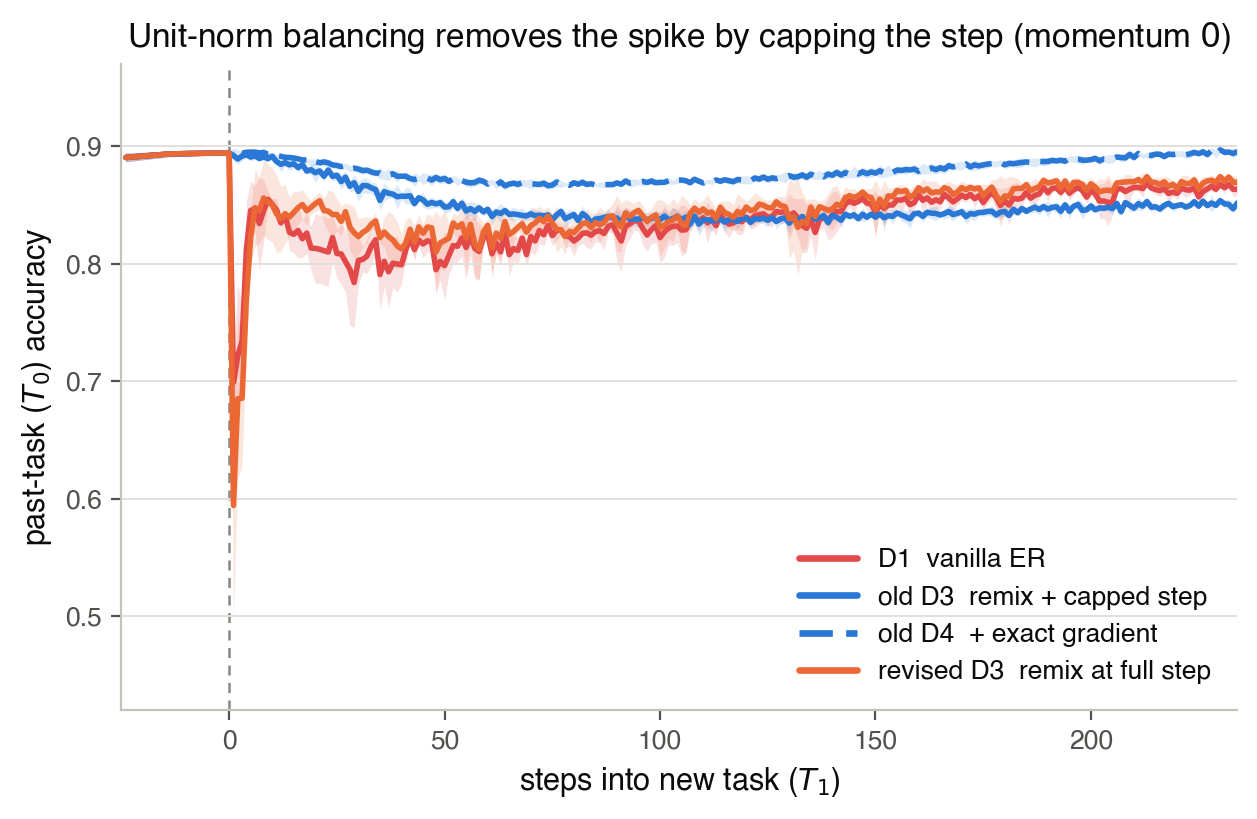
\includegraphics[width=0.72\linewidth]{img/results/D/old_balanced_t0.png}
    \caption{Per-step past-task ($T_0$) accuracy across the rot-MNIST switch at momentum $0$: vanilla ER (red), the original unit-norm balanced conditions (blue; dashed: exact gradient), and the revised balanced-direction condition at vanilla's step length (orange). The original conditions show no boundary spike because the unit normalisation caps the step exactly where the raw gradient is large; the same remix at full step length deepens the spike instead.}
    \label{fig:old_balanced}
\end{figure}

\begin{table}[H]
    \centering
    \scriptsize
    \setlength{\tabcolsep}{4pt}
    \resizebox{\textwidth}{!}{%
        \begin{tabular}{l ccc cc c cc c}
            \hline
            Condition            & ACC                 & FORG                 & min-ACC             & $\mathrm{WF}_{100}$ & $\mathrm{WP}_{100}$ & WC-ACC              & Depth            & Area end        & Recov.           \\
            \hline
            \multicolumn{10}{l}{\emph{Momentum $0.0$}}                                                                                                                                                                        \\
            old D3 unit-norm balanced & 0.849\,$\pm$\,0.005 & 0.031\,$\pm$\,0.018  & 0.824\,$\pm$\,0.006 & 0.045\,$\pm$\,0.002 & 0.721\,$\pm$\,0.004 & 0.836\,$\pm$\,0.004 & 5.7\,$\pm$\,1.9  & 1.4\,$\pm$\,0.4 & ---              \\
            old D4 fulldata unit-norm & 0.869\,$\pm$\,0.002 & -0.014\,$\pm$\,0.013 & 0.862\,$\pm$\,0.002 & 0.030\,$\pm$\,0.007 & 0.710\,$\pm$\,0.003 & 0.852\,$\pm$\,0.002 & 1.9\,$\pm$\,1.3  & 3.2\,$\pm$\,0.5 & ---              \\
            \hline
            \multicolumn{10}{l}{\emph{Momentum $0.9$}}                                                                                                                                                                        \\
            old D3 unit-norm balanced & 0.932\,$\pm$\,0.005 & 0.038\,$\pm$\,0.003  & 0.897\,$\pm$\,0.006 & 0.040\,$\pm$\,0.003 & 0.822\,$\pm$\,0.011 & 0.922\,$\pm$\,0.003 & 5.9\,$\pm$\,0.6  & 0.4\,$\pm$\,0.2 & ---              \\
            old D4 fulldata unit-norm & 0.967\,$\pm$\,0.001 & -0.022\,$\pm$\,0.003 & 0.942\,$\pm$\,0.005 & 0.016\,$\pm$\,0.004 & 0.834\,$\pm$\,0.010 & 0.950\,$\pm$\,0.002 & 1.3\,$\pm$\,0.4  & 0.2\,$\pm$\,0.1 & ---              \\
            \hline
        \end{tabular}%
    }
    \caption{The original unit-norm balanced conditions, full metrics. The
        low depths are produced by the step cap, not by the remix; see the
        text of this appendix and Section~\ref{subsec:res_levels}.}
    \label{tab:app_old_balanced}
\end{table}

\subsection{rot-MNIST: \texorpdfstring{$\lambda$}{lambda}-Curriculum (C-series)}
\label{app:curr_full}

\begin{table}[H]
    \centering
    \scriptsize
    \setlength{\tabcolsep}{4pt}
    \resizebox{\textwidth}{!}{%
        \begin{tabular}{l ccc cc c cc c}
            \hline
            Condition            & ACC                 & FORG                & min-ACC             & $\mathrm{WF}_{100}$ & $\mathrm{WP}_{100}$ & WC-ACC              & Depth            & Area end        & Recov.             \\
            \hline
            \multicolumn{10}{l}{\emph{Momentum $0.0$}}                                                                                                                                                                         \\
            C1 linear N50        & 0.851\,$\pm$\,0.023 & 0.042\,$\pm$\,0.021 & 0.707\,$\pm$\,0.019 & 0.148\,$\pm$\,0.011 & 0.748\,$\pm$\,0.006 & 0.784\,$\pm$\,0.021 & 17.5\,$\pm$\,1.7 & 4.9\,$\pm$\,0.5 & 35.8\,$\pm$\,6.3   \\
            C2 linear N100       & 0.844\,$\pm$\,0.025 & 0.046\,$\pm$\,0.023 & 0.719\,$\pm$\,0.033 & 0.140\,$\pm$\,0.025 & 0.730\,$\pm$\,0.006 & 0.786\,$\pm$\,0.019 & 16.2\,$\pm$\,4.3 & 3.6\,$\pm$\,0.3 & 64.0\,$\pm$\,8.6   \\
            C3 linear N200       & 0.828\,$\pm$\,0.025 & 0.054\,$\pm$\,0.024 & 0.739\,$\pm$\,0.048 & 0.128\,$\pm$\,0.043 & 0.688\,$\pm$\,0.004 & 0.784\,$\pm$\,0.034 & 14.3\,$\pm$\,4.6 & 1.8\,$\pm$\,0.6 & 132.8\,$\pm$\,43.4 \\
            C4 adaptive          & 0.833\,$\pm$\,0.025 & 0.050\,$\pm$\,0.019 & 0.754\,$\pm$\,0.025 & 0.111\,$\pm$\,0.016 & 0.703\,$\pm$\,0.007 & 0.794\,$\pm$\,0.020 & 12.8\,$\pm$\,2.9 & 2.2\,$\pm$\,0.5 & 88.8\,$\pm$\,6.1   \\
            C5 adaptive lmin0.05 & 0.835\,$\pm$\,0.025 & 0.048\,$\pm$\,0.019 & 0.749\,$\pm$\,0.027 & 0.113\,$\pm$\,0.016 & 0.702\,$\pm$\,0.006 & 0.793\,$\pm$\,0.020 & 13.2\,$\pm$\,3.2 & 2.2\,$\pm$\,0.5 & 88.8\,$\pm$\,6.1   \\
            C6 adaptive lmin0.10 & 0.836\,$\pm$\,0.026 & 0.048\,$\pm$\,0.021 & 0.743\,$\pm$\,0.026 & 0.120\,$\pm$\,0.019 & 0.700\,$\pm$\,0.007 & 0.791\,$\pm$\,0.019 & 13.9\,$\pm$\,3.3 & 2.4\,$\pm$\,0.5 & 88.4\,$\pm$\,11.0  \\
            C7 adaptive lmin0.20 & 0.837\,$\pm$\,0.031 & 0.049\,$\pm$\,0.024 & 0.743\,$\pm$\,0.030 & 0.119\,$\pm$\,0.023 & 0.710\,$\pm$\,0.010 & 0.792\,$\pm$\,0.024 & 13.9\,$\pm$\,3.4 & 2.7\,$\pm$\,0.6 & 64.8\,$\pm$\,8.2   \\
            \hline
            \multicolumn{10}{l}{\emph{Momentum $0.9$}}                                                                                                                                                                         \\
            C1 linear N50        & 0.932\,$\pm$\,0.003 & 0.053\,$\pm$\,0.005 & 0.892\,$\pm$\,0.004 & 0.041\,$\pm$\,0.004 & 0.830\,$\pm$\,0.012 & 0.927\,$\pm$\,0.003 & 6.4\,$\pm$\,0.5  & 0.2\,$\pm$\,0.1 & ---                \\
            C2 linear N100       & 0.932\,$\pm$\,0.003 & 0.051\,$\pm$\,0.008 & 0.892\,$\pm$\,0.005 & 0.036\,$\pm$\,0.003 & 0.826\,$\pm$\,0.012 & 0.926\,$\pm$\,0.002 & 6.4\,$\pm$\,0.6  & 0.2\,$\pm$\,0.1 & ---                \\
            C3 linear N200       & 0.925\,$\pm$\,0.007 & 0.051\,$\pm$\,0.006 & 0.893\,$\pm$\,0.004 & 0.031\,$\pm$\,0.004 & 0.819\,$\pm$\,0.010 & 0.920\,$\pm$\,0.006 & 6.2\,$\pm$\,0.6  & 0.1\,$\pm$\,0.0 & ---                \\
            C4 adaptive          & 0.917\,$\pm$\,0.001 & 0.019\,$\pm$\,0.004 & 0.931\,$\pm$\,0.005 & 0.016\,$\pm$\,0.003 & 0.798\,$\pm$\,0.010 & 0.915\,$\pm$\,0.001 & 2.5\,$\pm$\,0.5  & 0.3\,$\pm$\,0.1 & ---                \\
            C5 adaptive lmin0.05 & 0.922\,$\pm$\,0.001 & 0.023\,$\pm$\,0.004 & 0.930\,$\pm$\,0.005 & 0.016\,$\pm$\,0.002 & 0.802\,$\pm$\,0.009 & 0.921\,$\pm$\,0.001 & 2.6\,$\pm$\,0.5  & 0.1\,$\pm$\,0.0 & ---                \\
            C6 adaptive lmin0.10 & 0.927\,$\pm$\,0.002 & 0.028\,$\pm$\,0.005 & 0.926\,$\pm$\,0.004 & 0.017\,$\pm$\,0.003 & 0.806\,$\pm$\,0.009 & 0.927\,$\pm$\,0.002 & 3.0\,$\pm$\,0.4  & 0.0\,$\pm$\,0.0 & ---                \\
            C7 adaptive lmin0.20 & 0.931\,$\pm$\,0.002 & 0.035\,$\pm$\,0.005 & 0.919\,$\pm$\,0.003 & 0.021\,$\pm$\,0.004 & 0.812\,$\pm$\,0.009 & 0.930\,$\pm$\,0.001 & 3.7\,$\pm$\,0.4  & 0.0\,$\pm$\,0.0 & ---                \\
            \hline
        \end{tabular}%
    }
    \caption{rot-MNIST $\lambda$-curriculum sweep, full metrics, at both momentum
        settings. All conditions applied on top of standard ER (1\,k reservoir).}
    \label{tab:app_curr}
\end{table}

\paragraph{Full-buffer momentum diagnostic (C8).}
Table~\ref{tab:res_c8} crosses the practical curriculum with the full $60$k buffer
at both momentum settings, isolating momentum's two roles (Section~\ref{subsec:res_scalar}).
Source variance reduction alone (C8, full buffer, $\mu{=}0$) already closes the
gap to $0.2$ pp, so the residual the curriculum leaves at $\mu{=}0$ is estimator
variance, not structure; momentum's gap-closing role is interchangeable with the
full buffer. Acceleration alone (the $\mu{=}0.9$ column) restores accuracy: C8$_M$
reaches $0.955$, approaching the full-data ceiling (D2$_M$: $0.964$), while
re-introducing a small transient ($2.0$ pp, area $0.38$). The shape and timing
of this transient point to the $\lambda_{\min}$ floor meeting momentum. With
the replay gradient exact and the arc removed, the only push left in the first
steps is the floored fifth of the new-task gradient (the logged gradient-norm
ratio confirms the schedule sits at $\lambda = 0.2$ through the dip window),
and momentum amplifies a persistent push toward $1/(1-\mu) = 10$ times its
per-step size: the dip accordingly opens at the boundary, bottoms out about
ten steps in, and closes within about fifty as the replay gradient reasserts
itself. The floor is by construction the one share of the push the source gate
does not attenuate, so momentum briefly re-inflates exactly that share, a
miniature of the directional gate's re-inflation. The dose-response on the
same exact buffer supports the reading: the floored push without momentum
costs $0.2$ pp (C8), with momentum $2.0$ pp (C8$_M$), and the unfloored
abrupt switch with momentum $14.9$ pp (D2$_M$). C8$_M$'s area additionally
counts in full under the end-referencing convention of
Section~\ref{subsec:metrics}, since it recovers above its pre-switch level. C8/C8$_M$ are diagnostic probes: the full buffer defeats the limited-memory
premise, and the practical scalar-gate configuration remains C7$_M$
($3.7$ pp / $0.03$ / $0.931$) at $1/60$th the memory.

\begin{table}[H]
    \centering
    \small
    \begin{tabular}{l cccc}
        \hline
                                 & C7              & C7$_M$            & C8                & C8$_M$              \\
                                 & (1k, $\mu{=}0$) & (1k, $\mu{=}0.9$) & (full, $\mu{=}0$) & (full, $\mu{=}0.9$) \\
        \hline
        \texttt{gap\_depth} (pp) & $13.9$          & $3.7$             & $\mathbf{0.2}$    & $2.0$               \\
        \texttt{gap\_area\_end}  & $2.7$           & $0.03$            & $\mathbf{0.05}$   & $0.38$              \\
        ACC                      & $0.837$         & $0.931$           & $0.818$           & $\mathbf{0.955}$    \\
        \hline
    \end{tabular}
    \caption{Curriculum $\times$ full buffer $\times$ momentum on rot-MNIST,
        isolating momentum's two roles. Source variance reduction alone (C8) closes
        the gap; acceleration alone (the $\mu$ column) restores accuracy. The residual
        at C7 ($\mu{=}0$) is variance, not structure.}
    \label{tab:res_c8}
\end{table}

\subsection{rot-MNIST: Buffer-Fidelity Diagnostics}
\label{app:grad_full}

The gradient diagnostics of Appendix~\ref{subsubsec:grad_metrics} were logged for
the decomposition block only. The full-data conditions (D2, D4) reach exact
fidelity by construction, the replay gradient equals the deterministic
empirical past-task gradient, so cosine and magnitude ratio are $1.000$. The
finite-buffer conditions (D1, D3) show the directional and magnitude error a
$1{,}000$-sample reservoir incurs against $g_{\text{true}}$.

\begin{table}[H]
    \centering
    \scriptsize
    \setlength{\tabcolsep}{4pt}
    \begin{tabular}{l ccc}
        \hline
        Condition                 & $\bar{\cos}$        & $\cos_{\min}$        & $\bar{\rho}$        \\
        \hline
        D1 vanilla ($\mu{=}0$)    & 0.711\,$\pm$\,0.035 & 0.086\,$\pm$\,0.103  & 1.040\,$\pm$\,0.039 \\
        D3 balanced ($\mu{=}0$)   & 0.665\,$\pm$\,0.043 & 0.025\,$\pm$\,0.140  & 1.137\,$\pm$\,0.060 \\
        D1 vanilla ($\mu{=}0.9$)  & 0.551\,$\pm$\,0.033 & 0.135\,$\pm$\,0.069  & 0.418\,$\pm$\,0.014 \\
        D3 balanced ($\mu{=}0.9$) & 0.441\,$\pm$\,0.039 & -0.052\,$\pm$\,0.117 & 0.265\,$\pm$\,0.024 \\
        D2, D4 (full data)        & 1.000               & 1.000                & 1.000               \\
        \hline
    \end{tabular}
    \caption{Buffer-fidelity diagnostics for the decomposition block:
        $\bar{\cos}$ and $\cos_{\min}$ are the mean and minimum of
        $\cos(g_{\text{replay}}, g_{\text{true}})$ over the window; $\bar{\rho}$ is the
        mean of $\|g_{\text{replay}}\|/\|g_{\text{true}}\|$.}
    \label{tab:app_grad}
\end{table}

\subsection{rot-MNIST: Asymmetric PER (P-series)}
\label{app:per_full}

Table~\ref{tab:app_per_full} gives the full metric set for the asymmetric-PER
$\delta$ sweep on both buffer legs and at both momentum settings; the momentum-$0$
depth/area/ACC columns match Table~\ref{tab:res_per} in the main text, and the
momentum-$0.9$ rows are the source of the re-inflation numbers of
Section~\ref{subsec:res_directional}. Momentum-$0.9$ runs cover the three
strongest filters on the standard leg and $\delta \in \{0.3, 0.1\}$ on the
full-buffer leg.

\begin{table}[H]
    \centering
    \scriptsize
    \setlength{\tabcolsep}{4pt}
    \resizebox{\textwidth}{!}{%
        \begin{tabular}{l ccc cc c cc}
            \hline
            Condition                 & ACC                 & FORG                 & min-ACC             & $\mathrm{WF}_{100}$ & $\mathrm{WP}_{100}$ & WC-ACC              & Depth             & Area end          \\
            \hline
            \multicolumn{9}{l}{\emph{Standard ($1$k) buffer, momentum $0.0$}}                                                                                                                                      \\
            $\delta{=}1.0$            & 0.869\,$\pm$\,0.005 & 0.027\,$\pm$\,0.018  & 0.792\,$\pm$\,0.012 & 0.081\,$\pm$\,0.009 & 0.733\,$\pm$\,0.009 & 0.838\,$\pm$\,0.006 & 9.0\,$\pm$\,0.6   & 3.29\,$\pm$\,0.65 \\
            $\delta{=}0.3$            & 0.873\,$\pm$\,0.004 & 0.023\,$\pm$\,0.017  & 0.807\,$\pm$\,0.012 & 0.068\,$\pm$\,0.009 & 0.736\,$\pm$\,0.008 & 0.847\,$\pm$\,0.005 & 7.4\,$\pm$\,1.1   & 2.32\,$\pm$\,0.59 \\
            $\delta{=}0.1$            & 0.876\,$\pm$\,0.004 & 0.018\,$\pm$\,0.016  & 0.822\,$\pm$\,0.012 & 0.056\,$\pm$\,0.009 & 0.739\,$\pm$\,0.008 & 0.856\,$\pm$\,0.005 & 5.9\,$\pm$\,1.5   & 1.56\,$\pm$\,0.65 \\
            $\delta{=}0.03$           & 0.880\,$\pm$\,0.005 & 0.012\,$\pm$\,0.015  & 0.834\,$\pm$\,0.012 & 0.048\,$\pm$\,0.005 & 0.741\,$\pm$\,0.007 & 0.862\,$\pm$\,0.005 & 4.8\,$\pm$\,1.9   & 1.04\,$\pm$\,0.58 \\
            \multicolumn{9}{l}{\emph{Standard ($1$k) buffer, momentum $0.9$}}                                                                                                                                      \\
            $\delta{=}0.3$            & 0.929\,$\pm$\,0.002 & 0.061\,$\pm$\,0.004  & 0.851\,$\pm$\,0.008 & 0.065\,$\pm$\,0.004 & 0.813\,$\pm$\,0.009 & 0.907\,$\pm$\,0.005 & 10.4\,$\pm$\,0.5  & 0.50\,$\pm$\,0.17 \\
            $\delta{=}0.1$            & 0.928\,$\pm$\,0.002 & 0.061\,$\pm$\,0.006  & 0.861\,$\pm$\,0.008 & 0.060\,$\pm$\,0.005 & 0.815\,$\pm$\,0.009 & 0.911\,$\pm$\,0.005 & 9.4\,$\pm$\,0.5   & 0.38\,$\pm$\,0.19 \\
            $\delta{=}0.03$           & 0.929\,$\pm$\,0.003 & 0.060\,$\pm$\,0.009  & 0.871\,$\pm$\,0.008 & 0.053\,$\pm$\,0.007 & 0.816\,$\pm$\,0.010 & 0.917\,$\pm$\,0.005 & 8.5\,$\pm$\,0.6   & 0.23\,$\pm$\,0.12 \\
            \hline
            \multicolumn{9}{l}{\emph{Full ($60$k) buffer, momentum $0.0$}}                                                                                                                                         \\
            $\delta{=}1.0$            & 0.898\,$\pm$\,0.002 & -0.025\,$\pm$\,0.012 & 0.841\,$\pm$\,0.011 & 0.037\,$\pm$\,0.011 & 0.734\,$\pm$\,0.006 & 0.865\,$\pm$\,0.006 & 4.0\,$\pm$\,1.0   & 2.32\,$\pm$\,1.38 \\
            $\delta{=}0.3$            & 0.900\,$\pm$\,0.002 & -0.029\,$\pm$\,0.012 & 0.867\,$\pm$\,0.002 & 0.026\,$\pm$\,0.007 & 0.739\,$\pm$\,0.005 & 0.878\,$\pm$\,0.002 & 1.5\,$\pm$\,1.1   & 1.01\,$\pm$\,0.91 \\
            $\delta{=}0.1$            & 0.901\,$\pm$\,0.002 & -0.032\,$\pm$\,0.013 & 0.860\,$\pm$\,0.026 & 0.040\,$\pm$\,0.028 & 0.741\,$\pm$\,0.004 & 0.875\,$\pm$\,0.013 & 2.2\,$\pm$\,1.6   & 0.44\,$\pm$\,0.38 \\
            $\delta{=}0.03$           & 0.903\,$\pm$\,0.002 & -0.035\,$\pm$\,0.012 & 0.787\,$\pm$\,0.094 & 0.118\,$\pm$\,0.102 & 0.742\,$\pm$\,0.004 & 0.838\,$\pm$\,0.048 & 9.5\,$\pm$\,8.2   & 0.43\,$\pm$\,0.25 \\
            $\delta{=}0.03$ (CG $60$) & 0.903\,$\pm$\,0.002 & -0.035\,$\pm$\,0.012 & 0.766\,$\pm$\,0.113 & 0.126\,$\pm$\,0.109 & 0.742\,$\pm$\,0.004 & 0.828\,$\pm$\,0.057 & 11.5\,$\pm$\,10.1 & 0.47\,$\pm$\,0.28 \\
            \multicolumn{9}{l}{\emph{Full ($60$k) buffer, momentum $0.9$}}                                                                                                                                         \\
            $\delta{=}0.3$            & 0.964\,$\pm$\,0.001 & -0.012\,$\pm$\,0.002 & 0.864\,$\pm$\,0.009 & 0.052\,$\pm$\,0.005 & 0.813\,$\pm$\,0.008 & 0.913\,$\pm$\,0.005 & 9.1\,$\pm$\,0.8   & 1.91\,$\pm$\,0.26 \\
            $\delta{=}0.1$            & 0.965\,$\pm$\,0.001 & -0.012\,$\pm$\,0.003 & 0.880\,$\pm$\,0.008 & 0.044\,$\pm$\,0.004 & 0.814\,$\pm$\,0.008 & 0.921\,$\pm$\,0.005 & 7.6\,$\pm$\,0.7   & 1.57\,$\pm$\,0.25 \\
            \hline
        \end{tabular}%
    }
    \caption{rot-MNIST asymmetric-PER $\delta$ sweep, full metrics: both buffer
        legs at both momentum settings, plus the solver control (CG $60$). The
        momentum-$0.9$ rows show the re-inflation of
        Section~\ref{subsec:res_directional}: depth climbs on every leg relative to
        its momentum-$0$ counterpart, while the full-buffer accuracies
        (${\approx}0.965$) are diagnostic values only, the full buffer defeating the limited-memory premise.}
    \label{tab:app_per_full}
\end{table}

\subsection{rot-MNIST: Symmetric vs.\ Asymmetric Preconditioning}
\label{app:per_sym}

Leaving the restoring gradient $g_{\text{rep}}$ at full strength is the directional
gate's defining choice (Section~\ref{subsec:res_directional}). The alternative is to
precondition the summed update, $d = \delta(F_{\text{rep}}+\delta I)^{-1}(g_{\text{cur}}+g_{\text{rep}})$,
the symmetric variant that passes both gradients through the same metric. Because
$g_{\text{rep}}$ is the gradient of the replay loss, it lies in the top eigenspace of that
loss's own Fisher $F_{\text{rep}}$, so the symmetric filter shrinks the restoring
gradient \emph{harder} than the harmful push it is meant to brake and cannot
preferentially protect the past task. Table~\ref{tab:res_per_sym} sweeps the same
$\delta$ on both variants, and they are mirror images. As the filter strengthens
($\delta \to 0$) the asymmetric gate's forgetting falls (FORG $0.027 \to 0.012$) and its
accuracy rises, while the symmetric gate's forgetting \emph{climbs} ($0.030 \to 0.066$)
and its accuracy falls; every one of these four trends holds across all five seeds.
Symmetric depth barely moves across the sweep ($5.7 \to 6.7$ pp) and at $\delta{=}1.0$
even sits below the asymmetric gate's ($5.7$ vs.\ $9.0$ pp), because filtering the whole
update also damps the per-step \emph{expression} of the dip. This is the area caveat of
Section~\ref{subsec:metrics} made concrete: the symmetric gate's end-referenced area
collapses toward zero ($2.7 \to 0.01$) not because the dip recovers but because it stops
recovering, settling into a permanent accommodation that the area excludes and the
forgetting metric records. Read on depth or transient area the symmetric gate looks
competitive; read on forgetting and final accuracy it degrades monotonically as its
filter strengthens. Asymmetry is what turns the filter from a reshuffling of the damage
into a net removal of it.

\begin{table}[H]
    \centering
    \small
    \begin{tabular}{l cccc c cccc}
        \hline
                 & \multicolumn{4}{c}{Asymmetric ($g_{\text{rep}}$ free)} &           & \multicolumn{4}{c}{Symmetric (joint)}                                                              \\
        \cline{2-5}\cline{7-10}
        $\delta$ & depth (pp)                                             & area      & FORG                                  & ACC     &  & depth (pp) & area   & FORG    & ACC     \\
        \hline
        $1.0$    & $9.0$                                                  & $3.29$    & $0.027$                               & $0.869$ &  & $5.7$      & $2.69$ & $0.030$ & $0.872$ \\
        $0.3$    & $7.4$                                                  & $2.32$    & $0.023$                               & $0.873$ &  & $5.9$      & $1.65$ & $0.042$ & $0.867$ \\
        $0.1$    & $5.9$                                                  & $1.56$    & $0.018$                               & $0.876$ &  & $6.2$      & $0.34$ & $0.057$ & $0.861$ \\
        $0.03$   & $4.8$                                                  & $1.04$    & $0.012$                               & $0.880$ &  & $6.7$      & $0.01$ & $0.066$ & $0.857$ \\
        \hline
    \end{tabular}
    \caption{Asymmetric versus symmetric preconditioning on the standard $1$k buffer at
        momentum $0$, five seeds, sweeping the shared damping $\delta$. Both variants filter
        through the replay Fisher $F_{\text{rep}}$; they differ only in whether the metric is
        applied to the new-task push alone (asymmetric, $g_{\text{rep}}$ left free) or to the
        summed update (symmetric). As $\delta \to 0$ the asymmetric gate improves on every
        axis while the symmetric gate degrades on every axis; symmetric depth stays flat
        because the filter suppresses the per-step expression of the dip even as the
        underlying forgetting grows, and the symmetric end-referenced area collapses
        toward zero for the same reason: the past task stops recovering, so the loss
        registers in FORG rather than in the transient area (Section~\ref{subsec:metrics}).}
    \label{tab:res_per_sym}
\end{table}

\subsection{CIFAR-10: Headline Block}
\label{app:cifar_headline_full}

\begin{table}[H]
    \centering
    \scriptsize
    \setlength{\tabcolsep}{4pt}
    \resizebox{\textwidth}{!}{%
        \begin{tabular}{l ccc cc c cc}
            \hline
            Condition        & ACC                 & FORG                 & min-ACC             & $\mathrm{WF}_{100}$ & $\mathrm{WP}_{100}$ & WC-ACC              & Depth             & Area end          \\
            \hline
            G1 vanilla BN    & 0.723\,$\pm$\,0.008 & 0.010\,$\pm$\,0.019  & 0.644\,$\pm$\,0.023 & 0.127\,$\pm$\,0.015 & 0.484\,$\pm$\,0.020 & 0.667\,$\pm$\,0.016 & 11.8\,$\pm$\,2.5  & 17.5\,$\pm$\,4.6  \\
            G2 adaptive BN   & 0.722\,$\pm$\,0.011 & 0.006\,$\pm$\,0.016  & 0.713\,$\pm$\,0.017 & 0.070\,$\pm$\,0.010 & 0.469\,$\pm$\,0.016 & 0.698\,$\pm$\,0.013 & 4.8\,$\pm$\,0.7   & 3.6\,$\pm$\,2.2   \\
            G3 asym.\ PER BN & 0.715\,$\pm$\,0.011 & -0.008\,$\pm$\,0.018 & 0.698\,$\pm$\,0.023 & 0.124\,$\pm$\,0.022 & 0.460\,$\pm$\,0.025 & 0.682\,$\pm$\,0.023 & 5.9\,$\pm$\,4.3   & 3.3\,$\pm$\,3.0   \\
            G4 vanilla GN    & 0.730\,$\pm$\,0.011 & -0.023\,$\pm$\,0.030 & 0.309\,$\pm$\,0.111 & 0.294\,$\pm$\,0.097 & 0.415\,$\pm$\,0.058 & 0.507\,$\pm$\,0.054 & 41.2\,$\pm$\,13.5 & 34.9\,$\pm$\,23.7 \\
            G5 adaptive GN   & 0.731\,$\pm$\,0.020 & -0.026\,$\pm$\,0.026 & 0.670\,$\pm$\,0.055 & 0.095\,$\pm$\,0.033 & 0.340\,$\pm$\,0.052 & 0.687\,$\pm$\,0.037 & 5.2\,$\pm$\,2.1   & 1.7\,$\pm$\,0.9   \\
            G6 asym.\ PER GN & 0.741\,$\pm$\,0.009 & -0.035\,$\pm$\,0.018 & 0.673\,$\pm$\,0.023 & 0.080\,$\pm$\,0.009 & 0.330\,$\pm$\,0.024 & 0.696\,$\pm$\,0.015 & 5.6\,$\pm$\,1.1   & 4.8\,$\pm$\,3.8   \\
            \hline
        \end{tabular}%
    }
    \caption{CIFAR-10 headline block, full metrics (ResNet-18, momentum $0.9$,
        buffer $5{,}000$, five seeds). ``adaptive'' is the practical curriculum with
        $\lambda_{\min} = 0.20$; ``asym.\ PER'' runs at $\delta = 0.1$.}
    \label{tab:app_cifar_headline}
\end{table}

\paragraph{The gates' residual batch-norm dip.}
The small gap the gates keep under batch norm is a genuine boundary transient:
in Figure~\ref{fig:cifar_curves}(a) both gated curves dip together over the
first steps after the switch, by roughly the tabulated $5$ pp, and recover to
their plateau within a few tens of steps. A reading consistent with this
pattern is the normalisation pathway of Section~\ref{subsec:cifar}. BatchNorm's
running statistics update on every forward pass, whatever the gate does to the
gradient, so the first corrupted batches shift them away from the clean task
and no gate on the update can hold that back; the clean replay samples in every
batch pull the statistics back, which matches the fast recovery. The group-norm
contrast supports the reading: with no cross-batch statistics to disturb, the
curriculum holds $T_0$ flat through the same boundary
(Figure~\ref{fig:cifar_curves}(b)) and its transient area falls to roughly half
its batch-norm value ($1.7$ vs.\ $3.6$). This is a reading rather than an
established mechanism; a control that freezes the running statistics across
the switch would isolate it.

\subsection{CIFAR-10: Generalisation Block}
\label{app:cifar_gen_full}

Each shift pairs the practical curriculum (``curric.'': adaptive $\lambda_{\min} =
    0.20$, buffer $5{,}000$) against a vanilla-ER control on the same shift, at the
indicated normalisation, over three seeds.

\begin{table}[H]
    \centering
    \scriptsize
    \setlength{\tabcolsep}{4pt}
    \begin{tabular}{l ccc c cc}
        \hline
        Condition              & ACC                 & FORG                 & min-ACC             & WC-ACC              & Depth             & Area end          \\
        \hline
        \multicolumn{7}{l}{\emph{BatchNorm}}                                                                                                                    \\
        shot noise (vanilla) & 0.724\,$\pm$\,0.011 & 0.017\,$\pm$\,0.010  & 0.633\,$\pm$\,0.017 & 0.663\,$\pm$\,0.014 & 13.1\,$\pm$\,3.0  & 21.2\,$\pm$\,3.9  \\
        shot noise (curric.) & 0.723\,$\pm$\,0.014 & 0.010\,$\pm$\,0.010  & 0.708\,$\pm$\,0.032 & 0.697\,$\pm$\,0.016 & 5.6\,$\pm$\,1.0   & 5.8\,$\pm$\,1.5   \\
        contrast (vanilla)   & 0.671\,$\pm$\,0.026 & -0.008\,$\pm$\,0.006 & 0.610\,$\pm$\,0.063 & 0.586\,$\pm$\,0.048 & 15.4\,$\pm$\,3.9  & 33.4\,$\pm$\,4.5  \\
        contrast (curric.)   & 0.671\,$\pm$\,0.044 & -0.012\,$\pm$\,0.007 & 0.727\,$\pm$\,0.034 & 0.643\,$\pm$\,0.048 & 3.7\,$\pm$\,1.1   & 2.2\,$\pm$\,0.9   \\
        3-task (vanilla)     & 0.740\,$\pm$\,0.006 & -0.011\,$\pm$\,0.013 & 0.670\,$\pm$\,0.015 & 0.691\,$\pm$\,0.010 & 3.3\,$\pm$\,0.4   & 6.0\,$\pm$\,0.7   \\
        3-task (curric.)     & 0.745\,$\pm$\,0.010 & -0.021\,$\pm$\,0.008 & 0.677\,$\pm$\,0.025 & 0.696\,$\pm$\,0.017 & 6.9\,$\pm$\,2.7   & 3.9\,$\pm$\,0.1   \\
        \hline
        \multicolumn{7}{l}{\emph{GroupNorm}}                                                                                                                    \\
        shot noise (vanilla) & 0.718\,$\pm$\,0.021 & -0.036\,$\pm$\,0.036 & 0.244\,$\pm$\,0.075 & 0.469\,$\pm$\,0.032 & 46.3\,$\pm$\,12.0 & 54.4\,$\pm$\,40.8 \\
        shot noise (curric.) & 0.705\,$\pm$\,0.061 & -0.028\,$\pm$\,0.012 & 0.638\,$\pm$\,0.108 & 0.656\,$\pm$\,0.087 & 7.3\,$\pm$\,5.9   & 2.4\,$\pm$\,1.1   \\
        contrast (vanilla)   & 0.777\,$\pm$\,0.022 & -0.067\,$\pm$\,0.021 & 0.641\,$\pm$\,0.061 & 0.710\,$\pm$\,0.040 & 8.4\,$\pm$\,4.4   & 3.3\,$\pm$\,0.6   \\
        contrast (curric.)   & 0.778\,$\pm$\,0.032 & -0.070\,$\pm$\,0.013 & 0.668\,$\pm$\,0.077 & 0.724\,$\pm$\,0.054 & 3.9\,$\pm$\,3.1   & 1.2\,$\pm$\,0.8   \\
        3-task (vanilla)     & 0.722\,$\pm$\,0.020 & -0.023\,$\pm$\,0.015 & 0.468\,$\pm$\,0.043 & 0.550\,$\pm$\,0.023 & 4.4\,$\pm$\,0.4   & 10.3\,$\pm$\,3.6  \\
        3-task (curric.)     & 0.721\,$\pm$\,0.019 & -0.025\,$\pm$\,0.020 & 0.421\,$\pm$\,0.114 & 0.517\,$\pm$\,0.070 & 32.8\,$\pm$\,14.5 & 32.0\,$\pm$\,19.5 \\
        \hline
    \end{tabular}
    \caption{CIFAR-10 generalisation block, full metrics. The two-task novel
        corruptions (shot noise, contrast) favour the curriculum under both
        normalisations; the three-task group-norm sequence is the outlier analysed
        below.}
    \label{tab:app_cifar_gen}
\end{table}

\paragraph{The three-task group-norm failure.}
The three-task sequence is the one place the curriculum underperforms its
control (depth $32.8 \pm 14.5$ pp against vanilla's $4.4 \pm 0.4$,
Table~\ref{tab:app_cifar_gen}; Figure~\ref{fig:failure_curves}), and the logged
gradient-norm traces locate the failure in the conditioning of the feedback
signal. The adaptive ratio $r = \|g_{\text{replay}}\|/\|g_{\text{new}}\|$
carries information through the boundary ordering of
Section~\ref{subsec:curriculum}: at a well-separated switch the new-task
gradient dwarfs the replay gradient, so $r$ starts near zero and its rise
tracks the replay gradient reasserting itself. The first boundary of this
sequence behaves that way (clean $\rightarrow$ Gaussian: first-step new-task
loss $1.9$--$2.1$, $r \approx 0.2$), and the schedule holds every past task
flat through it. The second boundary never establishes the ordering: Gaussian
and shot noise are near-identical, so the incoming model already fits the new
task ($T_2$ accuracy $0.67$--$0.71$ before its first step, new-task loss
$0.5$--$0.7$), leaving $\|g_{\text{new}}\|$ small, while
$\|g_{\text{replay}}\|$ is small because the model is converged on the
replayed tasks. The ratio becomes a quotient of two near-zero norms: under
group norm it reads $0.5$--$1.3$ from the first step and fluctuates step to
step, so the EMA drives $\lambda$ from the floor to ${\approx}0.7$--$0.8$
within fifty steps and back to $\lambda_{\min}$ within a few hundred. The gate
is moved by noise, not by damage.

What follows, in all three seeds, is not a stability gap but an optimisation
instability. Within the first forty steps the replay loss itself diverges
($0.2$--$0.4 \rightarrow 0.8$--$2.1$) and every task falls together,
\emph{including the one being trained} ($T_2$: $0.71 \rightarrow 0.29$,
$0.69 \rightarrow 0.30$, $0.67 \rightarrow 0.51$ across seeds), before the run
recovers; the per-seed depth scales with the divergence, which is where the
$\pm 14.5$ pp spread comes from. Because all tasks crash together, the depth
and area of the three-task group-norm rows record this instability, not the
past-task transient the rest of the study measures. Two controls isolate the
trigger. The vanilla run crosses the same boundary with a flat replay loss and
$4.4$ pp of depth, so the near-identical boundary is harmless on its own; the
batch-norm run executes the identical schedule through the same boundary, with
the same ill-conditioned early ratio, without instability
(Figure~\ref{fig:failure_curves}), so the noise-driven $\lambda$ is not
sufficient either. The failure needs both the unconditioned signal and the
group-norm backbone's boundary sensitivity, consistent with the far deeper
group-norm transients vanilla ER shows on the same corruption family (shot
noise: $46.3$ vs $13.1$ pp, Table~\ref{tab:app_cifar_gen}). We therefore read
the episode as a reliability boundary of the gradient-norm-ratio signal rather
than of the gate principle: the ratio loses its meaning when both norms become
small, and the design admits direct guards: freezing $\lambda$ when both
norms fall below a reference scale, or reading a damage signal that does not
vanish at a quiet boundary, such as the replay-loss excess over its pre-switch
level.

\begin{figure}[H]
    \centering
    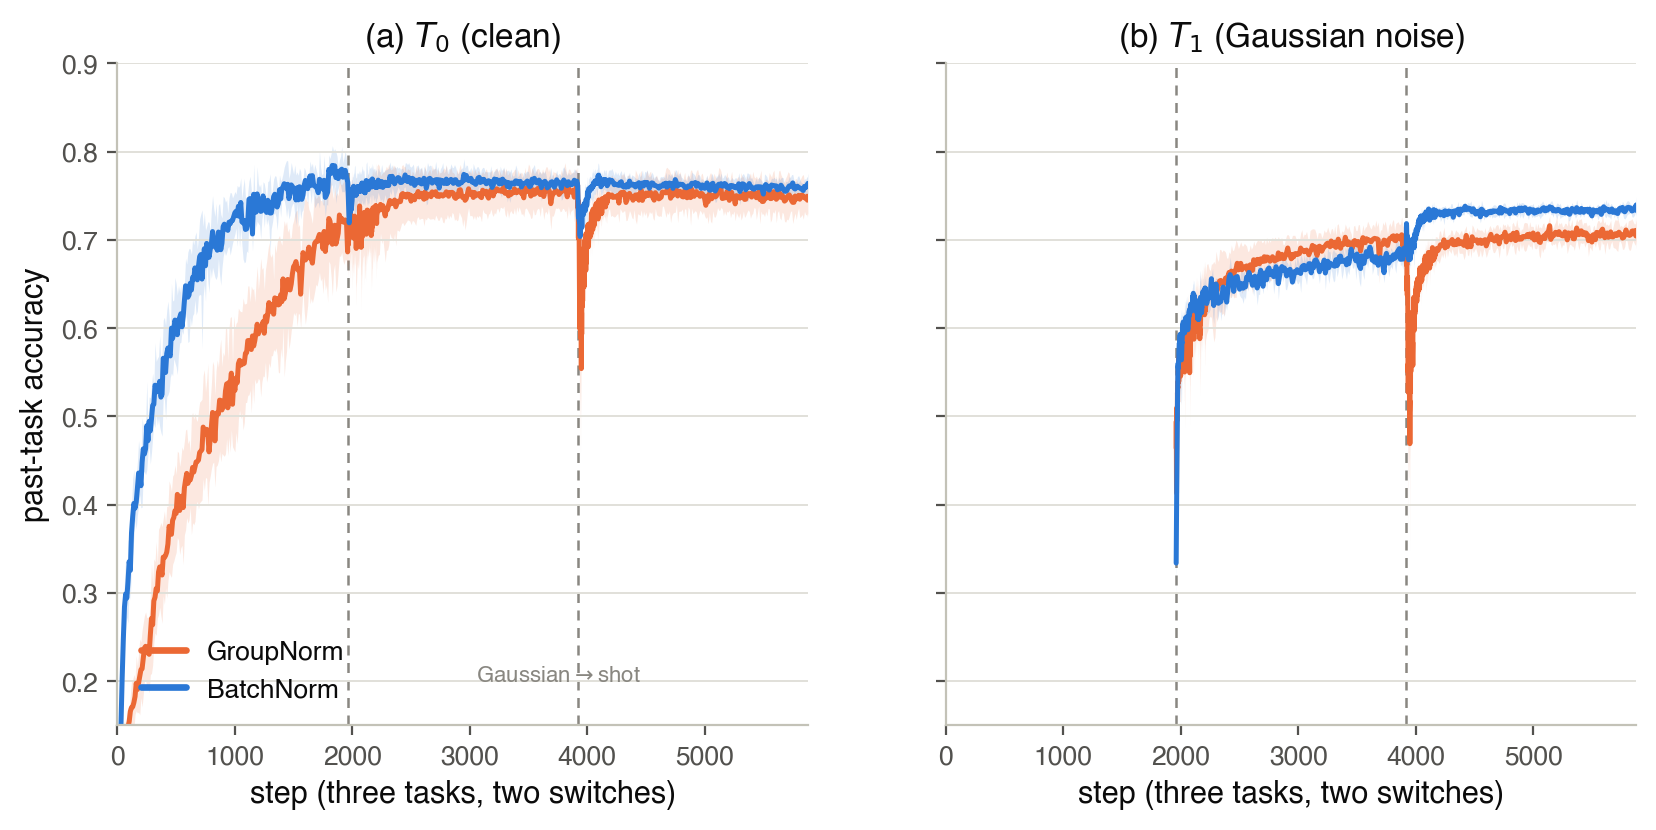
\includegraphics[width=\linewidth]{img/results/T/cifar_3task_failure.png}
    \caption{Per-step past-task accuracy across the three-task CIFAR-10
        generalisation sequence (none $\rightarrow$ Gaussian $\rightarrow$ shot,
        ResNet-18, practical curriculum, three seeds with $\pm$std bands), comparing
        the group-norm run (orange) against its batch-norm counterpart (blue). The
        two switches (dashed) fall at ${\sim}2$k and ${\sim}4$k steps. The first
        boundary (none $\rightarrow$ Gaussian) barely perturbs the past tasks in
        either norm. The second (Gaussian $\rightarrow$ shot, two near-identical
        corruptions) drives a deep transient in $T_0$ (a) and $T_1$ (b) under group
        norm only, while the batch-norm run holds flat through both switches. The dip
        is thus localised entirely to the second transition and to group norm, the
        adaptive-ratio reliability boundary analysed above.}
    \label{fig:failure_curves}
\end{figure}

\subsection{CIFAR-10: Momentum Cross and Compute Cost}
\label{app:cifar_extra}

This subsection collects the three deep-backbone checks summarised in
Section~\ref{subsec:res_cifar}: the momentum cross (Table~\ref{tab:res_cifar_mom}),
the generalisation block (Table~\ref{tab:app_cifar_gen} above), and the compute cost
(Table~\ref{tab:res_cost}).

\paragraph{Momentum cross.}
The cross repeats the composability test of Section~\ref{subsec:momentum} on the
ResNet, pairing momentum-$0$ runs at group norm against the momentum-$0.9$ rows,
and it turns out to be only weakly informative. At momentum $0$ the ResNet
under-converges the past task in ten epochs (vanilla min-ACC $0.11$, ACC $0.65$), so
every momentum-$0$ depth sits on a degraded baseline. On that baseline both gates
improve with momentum by similar margins (curriculum $28.6 \rightarrow 5.2$ pp,
asymmetric PER $22.6 \rightarrow 5.6$ pp), so the cross cannot separate the predicted
source-attenuation composition from a general convergence gain, and the prediction
that momentum re-inflates the directional gate does not appear; the vanilla null
($40.5 \rightarrow 41.2$ pp) is directionally consistent with the account but rests
on the same degraded baseline. We therefore draw no mechanism conclusion from this
cross in either direction: the momentum signatures rest on the rot-MNIST results,
where the MLP isolates them cleanly (Sections~\ref{subsec:res_scalar}
and~\ref{subsec:res_directional}), and a clean deep-backbone test would need a
converged momentum-$0$ baseline (Section~\ref{subsec:disc_limits}).

\begin{table}[H]
    \centering
    \small
    \begin{tabular}{l cc}
        \hline
        Method (GroupNorm)                   & depth, $\mu{=}0$ & depth, $\mu{=}0.9$ \\
        \hline
        Vanilla ER                           & $40.5 \pm 4.0$   & $41.2 \pm 13.5$    \\
        Curriculum ($\lambda_{\min}{=}0.20$) & $28.6 \pm 8.8$   & $5.2 \pm 2.1$      \\
        Asym.\ PER ($\delta{=}0.1$)          & $22.6 \pm 9.7$   & $5.6 \pm 1.1$      \\
        \hline
    \end{tabular}
    \caption{CIFAR-10 momentum cross (group norm, buffer $5{,}000$, five seeds), gap
        depth in pp. All momentum-$0$ cells sit on an under-converged baseline
        (vanilla min-ACC $0.11$), so the cross is read as uninformative for the
        momentum signatures rather than as partial confirmation (see text).}
    \label{tab:res_cifar_mom}
\end{table}

\paragraph{Compute cost.}
Cost is measured with a dedicated benchmark: one full two-task run per gate in its
headline configuration (curriculum: adaptive schedule, $\lambda_{\min}{=}0.20$;
asymmetric PER: $\delta{=}0.1$, $25$ warm-started CG iterations; momentum $0.9$,
group norm and buffer $5{,}000$ on CIFAR), five seeds each on a single NVIDIA RTX
PRO~6000, with per-step stability evaluation disabled so the numbers reflect method
compute alone. Wall-clock and CPU time come from \texttt{getrusage}; GPU utilisation,
power, and memory are sampled at $1$\,Hz with \texttt{nvidia-smi}, and energy is the
integrated power. On the ResNet-18 the split is stark (Table~\ref{tab:res_cost}). The
scalar gate adds one gradient-norm ratio and an EMA update to a standard ER step, and
its run is not even compute-bound: the GPU sits half-idle at $49\%$ utilisation and
$259$\,W. The directional gate's $25$ conjugate-gradient Fisher-vector products per
step, each on the order of a backward pass, saturate the same card ($96\%$, $367$\,W)
for $16\times$ as long, and since energy is power times time the two factors compound
to a $24\times$ energy gap ($13$ vs.\ $320$\,Wh per run). Memory is not the price:
peak GPU memory differs by $11\%$. On the rot-MNIST MLP both gates finish in under
half a minute at near-idle utilisation (the wall-clock is fixed startup, not method
compute), so no meaningful ratio exists there and the cost question is decided
entirely on the deep backbone. The ratios are the transferable claim; the absolute
numbers are specific to this card, and because ${\sim}15$--$30$\,s of each run is
startup, the training-only ratio is if anything slightly above $16\times$.

\begin{table}[H]
    \centering
    \small
    \begin{tabular}{ll ccccc}
        \hline
        Dataset & Gate & wall [s] & util [\%] & power [W] & energy [Wh] & mem [MB] \\
        \hline
        CIFAR-10 & Curriculum (scalar)         & $198 \pm 7$      & $49$    & $259$ & $13$  & $4{,}203$ \\
        (ResNet-18) & Asym.\ PER ($\delta{=}0.1$) & $3{,}157 \pm 11$ & $96$    & $367$ & $320$ & $4{,}679$ \\
        \hline
        rot-MNIST & Curriculum (scalar)         & $25 \pm 1$       & $<\!1$  & ---   & $0.4$ & $749$     \\
        (MLP) & Asym.\ PER ($\delta{=}0.1$) & $29 \pm 1$       & $8$     & ---   & $0.5$ & $769$     \\
        \hline
    \end{tabular}
    \caption{Compute cost of one full two-task run (mean over five seeds, $\pm$ sd on
        wall-clock; single RTX PRO 6000; per-step evaluation disabled): wall-clock, mean
        GPU utilisation and power, integrated GPU energy, and peak GPU memory. On the
        ResNet-18 the directional gate costs ${\sim}16\times$ the wall-clock and
        ${\sim}24\times$ the energy of the scalar gate at similar peak memory. The MLP
        rows are dominated by fixed startup on a near-idle GPU, so their power draw is
        idle draw (omitted) and no ratio is meaningful.}
    \label{tab:res_cost}
\end{table}

\subsection{Long-Sequence rot-MNIST (L-series)}
\label{app:longseq_full}

\begin{table}[H]
    \centering
    \scriptsize
    \setlength{\tabcolsep}{4pt}
    \resizebox{\textwidth}{!}{%
        \begin{tabular}{l ccc cc c cc}
            \hline
            Condition                             & ACC                 & FORG                & min-ACC             & $\mathrm{WF}_{100}$ & $\mathrm{WP}_{100}$ & WC-ACC              & Depth            & Area end          \\
            \hline
            \multicolumn{9}{l}{\emph{Momentum $0.0$}}                                                                                                                                                                        \\
            L1 vanilla ER                         & 0.861\,$\pm$\,0.004 & 0.060\,$\pm$\,0.004 & 0.670\,$\pm$\,0.055 & 0.207\,$\pm$\,0.053 & 0.443\,$\pm$\,0.011 & 0.722\,$\pm$\,0.043 & 21.0\,$\pm$\,5.8 & 3.14\,$\pm$\,0.77 \\
            L2 curriculum $\lambda_{\min}{=}0.20$ & 0.860\,$\pm$\,0.002 & 0.031\,$\pm$\,0.005 & 0.828\,$\pm$\,0.007 & 0.073\,$\pm$\,0.005 & 0.400\,$\pm$\,0.003 & 0.840\,$\pm$\,0.005 & 4.1\,$\pm$\,0.8  & 1.62\,$\pm$\,0.42 \\
            L3 asym.\ PER $\delta{=}0.1$          & 0.870\,$\pm$\,0.003 & 0.053\,$\pm$\,0.006 & 0.843\,$\pm$\,0.008 & 0.038\,$\pm$\,0.007 & 0.381\,$\pm$\,0.003 & 0.862\,$\pm$\,0.007 & 4.7\,$\pm$\,1.2  & 0.38\,$\pm$\,0.24 \\
            \hline
            \multicolumn{9}{l}{\emph{Momentum $0.9$}}                                                                                                                                                                        \\
            L1 vanilla ER                         & 0.889\,$\pm$\,0.007 & 0.096\,$\pm$\,0.008 & 0.845\,$\pm$\,0.007 & 0.065\,$\pm$\,0.008 & 0.317\,$\pm$\,0.006 & 0.870\,$\pm$\,0.006 & 8.9\,$\pm$\,1.7  & 1.68\,$\pm$\,0.69 \\
            L2 curriculum $\lambda_{\min}{=}0.20$ & 0.897\,$\pm$\,0.002 & 0.071\,$\pm$\,0.003 & 0.871\,$\pm$\,0.005 & 0.041\,$\pm$\,0.004 & 0.364\,$\pm$\,0.005 & 0.888\,$\pm$\,0.004 & 5.4\,$\pm$\,0.6  & 0.60\,$\pm$\,0.14 \\
            L3 asym.\ PER $\delta{=}0.1$          & 0.884\,$\pm$\,0.004 & 0.104\,$\pm$\,0.004 & 0.849\,$\pm$\,0.006 & 0.054\,$\pm$\,0.004 & 0.325\,$\pm$\,0.005 & 0.873\,$\pm$\,0.005 & 7.5\,$\pm$\,1.5  & 0.80\,$\pm$\,0.63 \\
            \hline
        \end{tabular}%
    }
    \caption{Five-task rot-MNIST (rotations $[0,30,60,90,120]^\circ$, four
        consecutive transitions, five seeds), the L-series: both gates in their
        practical configurations against vanilla ER, at both momentum settings.
        Depth is the worst single-boundary drop and area the end-referenced
        transient, aggregated as in the two-task blocks. At momentum $0$ both gates
        cut the depth from $21$ pp to ${\approx}4$ pp; under momentum the curriculum
        keeps the best cumulative retention while the re-inflated directional gate
        falls slightly behind vanilla on FORG ($0.104$ vs.\ $0.096$, all five seeds).}
    \label{tab:app_longseq}
\end{table}

\begin{figure}[H]
    \centering
    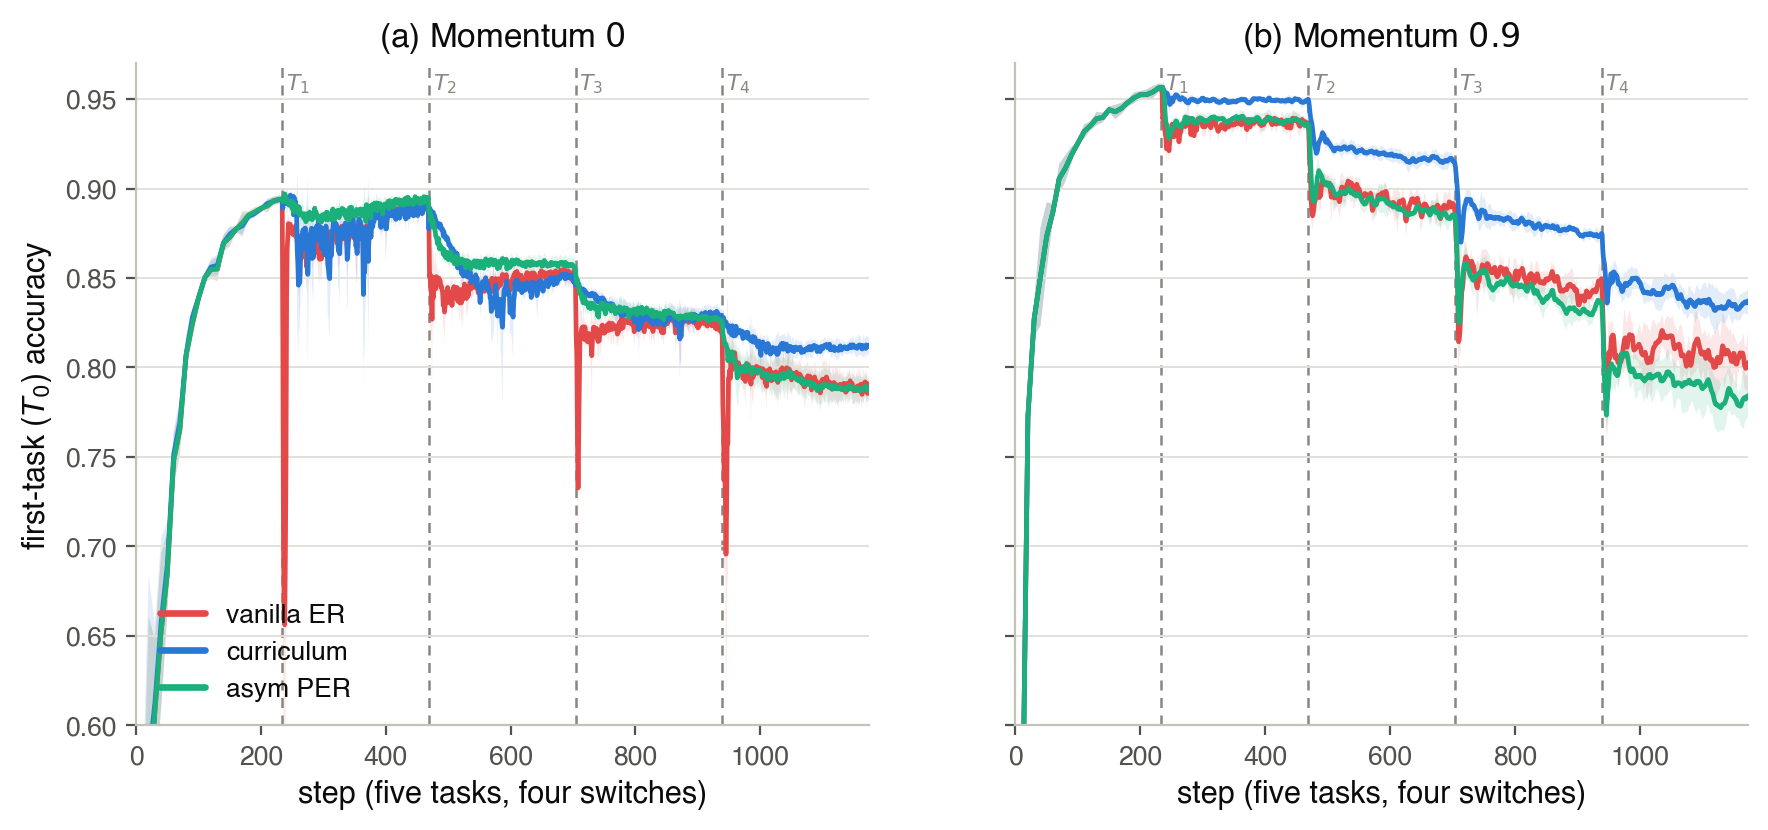
\includegraphics[width=\linewidth]{img/results/L/longseq.png}
    \caption{Five-task rot-MNIST (rotations $[0,30,60,90,120]^\circ$, four
        consecutive switches, five seeds with $\pm$std bands), the
        L-series: first-task $T_0$ accuracy across the whole sequence for vanilla ER
        (red), the practical curriculum $\lambda_{\min}{=}0.20$ (blue) and asymmetric
        PER $\delta{=}0.1$ (aqua); dashed lines mark the four switches, and the two
        panels are the two momentum settings. \textbf{(a) Momentum $0$:} both gates
        hold $T_0$ almost flat through every boundary, asymmetric PER the smoothest,
        while vanilla ER drops sharply at each switch. \textbf{(b) Momentum $0.9$:}
        PER's boundary transients return as momentum re-inflates its per-step filter
        (Section~\ref{subsec:res_directional}); the curriculum keeps the boundaries
        smoothest and holds the highest plateau (Table~\ref{tab:app_longseq}).}
    \label{fig:longseq}
\end{figure}

 % Complete Results
    \onecolumn
\section{Detailed Step-by-Step Derivation of the Trajectory Bound}
\label{app:detailed_proof}

\subsection*{Setup and Definitions}

\paragraph{1. The Combined Loss.}
The total loss function at any point $\lambda \in [0,1]$ in the curriculum is defined as:
\begin{equation}
    L_\lambda(\theta) = L_{\text{replay}}(\theta) + \lambda \cdot L_{\text{current}}(\theta)
\end{equation}

\paragraph{2. Defining the Hessians ($\nabla^2$).}
Differentiating the gradient once more gives the second-derivative matrix, the Hessian ($H$).
\begin{itemize}
    \item $H_{\text{replay}} = \nabla^2 L_{\text{replay}}(\theta)$ (The curvature of the old task)
    \item $H_{\text{current}} = \nabla^2 L_{\text{current}}(\theta)$ (The curvature of the new task)
\end{itemize}
Therefore, the Hessian of our combined loss, $H_\lambda$, is defined by applying the second derivative operator to the total loss function:
\begin{align*}
    H_\lambda & = \nabla^2 \left[ L_{\text{replay}}(\theta) + \lambda \cdot L_{\text{current}}(\theta) \right] \\
    H_\lambda & = \nabla^2 L_{\text{replay}}(\theta) + \lambda \cdot \nabla^2 L_{\text{current}}(\theta)       \\
    H_\lambda & = H_{\text{replay}} + \lambda \cdot H_{\text{current}}
\end{align*}

\paragraph{3. Assumption: Local-Minimum along the Interpolation Branch.}
We assume that the loss functions $L_{\text{replay}}$ and $L_{\text{current}}$ are twice continuously differentiable ($C^2$) in a neighbourhood of the interpolation path. Furthermore, we assume there exists a continuously differentiable ($C^1$) branch of critical points $\lambda \mapsto \Theta^*(\lambda)$ for the interpolated loss $L_\lambda$, initialized at $\Theta^*(0) = \theta_0^*$, such that the Hessian remains strictly positive-definite: $H_\lambda(\Theta^*(\lambda)) \succ 0$ for every $\lambda \in [0,1]$.

This assumption ensures that the iterate tracks a continuous family of strict local minima rather than relying on global convexity. Near $\lambda = 0$, this condition is naturally satisfied. Because the initial state $\theta_0^*$ is a non-degenerate local minimum of $L_{\text{replay}}$, it follows that $H_0 = H_{\text{replay}}(\theta_0^*) \succ 0$. Consequently, the implicit function theorem guarantees a unique smooth branch in the immediate neighbourhood of $\lambda = 0$.

The persistence of this positive-definite branch as $\lambda$ increases is bounded by Weyl's inequality applied to $H_\lambda = H_{\text{replay}} + \lambda H_{\text{current}}$; writing $\mu_{\min}(\cdot)$ for the smallest eigenvalue,
\begin{equation*}
    \mu_{\min}(H_\lambda) \;\ge\; \mu_{\min}(H_{\text{replay}}) + \lambda\, \mu_{\min}(H_{\text{current}}).
\end{equation*}
If the new task is locally convex at these points ($H_{\text{current}} \succeq 0$), positive-definiteness holds for all $\lambda \ge 0$ without requiring a global convexity assumption.

\subsection*{Part A: The Replay Loss Is Monotone Along the Reference Path}

Let $\Theta^*(\lambda)$ be the reference path, the exact parameter state that minimises $L_\lambda(\theta)$ for any given $\lambda$.

\paragraph{Step 1: The First-Order Condition.}
Because $\Theta^*(\lambda)$ is a minimum, the gradient of the total loss evaluated at that exact point must be zero:
\begin{align*}
    \nabla \left[ L_\lambda(\Theta^*(\lambda)) \right]                                                               & = 0 \\
    \nabla \left[ L_{\text{replay}}(\Theta^*(\lambda)) + \lambda \cdot L_{\text{current}}(\Theta^*(\lambda)) \right] & = 0
\end{align*}
Distributing the gradient operator to both terms gives us the fundamental First-Order Condition:
\begin{equation}
    \nabla L_{\text{replay}}(\Theta^*(\lambda)) + \lambda \cdot \nabla L_{\text{current}}(\Theta^*(\lambda)) = 0
    \label{eq:foc_detailed}
\end{equation}

\paragraph{Step 2: Implicit Differentiation to Find Path Movement.}
We want to know how the reference path $\Theta^*$ moves as $\lambda$ changes. We apply the derivative operator $\frac{d}{d\lambda}$ to the entire First-Order Condition:
\begin{equation*}
    \frac{d}{d\lambda} \left[ \nabla L_{\text{replay}}(\Theta^*(\lambda)) + \lambda \cdot \nabla L_{\text{current}}(\Theta^*(\lambda)) \right] = \frac{d}{d\lambda} [0]
\end{equation*}
Distributing the operator to each term:
\begin{equation*}
    \frac{d}{d\lambda} \left[ \nabla L_{\text{replay}}(\Theta^*(\lambda)) \right] + \frac{d}{d\lambda} \left[ \lambda \cdot \nabla L_{\text{current}}(\Theta^*(\lambda)) \right] = 0
\end{equation*}
Evaluating the first term via the multivariable chain rule:
\begin{equation*}
    \frac{d}{d\lambda} \left[ \nabla L_{\text{replay}}(\Theta^*(\lambda)) \right] = \nabla^2 L_{\text{replay}}(\Theta^*(\lambda)) \cdot \frac{d\Theta^*}{d\lambda}
\end{equation*}
Evaluating the second term via the product rule and chain rule:
\begin{equation*}
    \frac{d}{d\lambda} \left[ \lambda \cdot \nabla L_{\text{current}}(\Theta^*(\lambda)) \right] = (1) \cdot \nabla L_{\text{current}}(\Theta^*(\lambda)) + \lambda \cdot \left( \nabla^2 L_{\text{current}}(\Theta^*(\lambda)) \cdot \frac{d\Theta^*}{d\lambda} \right)
\end{equation*}
Substituting these expanded terms back into the equation:
\begin{equation*}
    \left[ \nabla^2 L_{\text{replay}}(\Theta^*) \cdot \frac{d\Theta^*}{d\lambda} \right] + \left[ \nabla L_{\text{current}}(\Theta^*) + \lambda \cdot \nabla^2 L_{\text{current}}(\Theta^*) \cdot \frac{d\Theta^*}{d\lambda} \right] = 0
\end{equation*}
Grouping the terms that share the path movement $\frac{d\Theta^*}{d\lambda}$:
\begin{equation*}
    \left( \nabla^2 L_{\text{replay}}(\Theta^*) + \lambda \cdot \nabla^2 L_{\text{current}}(\Theta^*) \right) \cdot \frac{d\Theta^*}{d\lambda} + \nabla L_{\text{current}}(\Theta^*) = 0
\end{equation*}
Recognising the definition of the combined Hessian $H_\lambda$ inside the parentheses:
\begin{equation*}
    H_\lambda \cdot \frac{d\Theta^*}{d\lambda} + \nabla L_{\text{current}}(\Theta^*(\lambda)) = 0
\end{equation*}
Solving algebraically for the path movement $\frac{d\Theta^*}{d\lambda}$:
\begin{equation}
    \frac{d\Theta^*}{d\lambda} = -H_\lambda^{-1} \cdot \nabla L_{\text{current}}(\Theta^*(\lambda))
    \label{eq:path_movement}
\end{equation}

\paragraph{Step 3: Calculating the Change in the Replay Loss.}
How does the replay loss change as $\lambda$ increases along this path? We apply the derivative operator:
\begin{equation*}
    \frac{d}{d\lambda} \left[ L_{\text{replay}}(\Theta^*(\lambda)) \right] = \nabla L_{\text{replay}}(\Theta^*(\lambda))^\top \cdot \frac{d\Theta^*(\lambda)}{d\lambda}
\end{equation*}
We perform two substitutions here. First, from \eqref{eq:foc_detailed}, we know $\nabla L_{\text{replay}} = -\lambda \cdot \nabla L_{\text{current}}$. Second, from \eqref{eq:path_movement}, we substitute the path movement.
\begin{align*}
    \frac{d}{d\lambda} L_{\text{replay}}(\Theta^*(\lambda)) & = \left( -\lambda \cdot \nabla L_{\text{current}}(\Theta^*(\lambda)) \right)^\top \cdot \left( -H_\lambda^{-1} \cdot \nabla L_{\text{current}}(\Theta^*(\lambda)) \right) \\
                                                            & = \lambda \cdot \nabla L_{\text{current}}(\Theta^*(\lambda))^\top \cdot H_\lambda^{-1} \cdot \nabla L_{\text{current}}(\Theta^*(\lambda))
\end{align*}
Because $H_\lambda$ is strictly positive-definite along the followed branch of local minima for all $\lambda \in [0,1]$ (per the Local-Minimum Assumption), its inverse $H_\lambda^{-1}$ is also positive-definite. The quadratic form $v^\top M v$ is therefore guaranteed to be non-negative. Since $\lambda \ge 0$, the entire equation satisfies:
\begin{equation*}
    \frac{d}{d\lambda} L_{\text{replay}}(\Theta^*(\lambda)) \ge 0
\end{equation*}
\emph{Conclusion for Part A:} The replay loss never decreases along the reference path, so it can never overshoot its final joint-optimum value.

\subsection*{Part B: The Iterate Tracks the Reference Path with $O(1/N)$ Lag}

Let $\theta(t)$ be the actual position of the model parameters at time $t$. We define the tracking error $e(t)$ (written $e$ to avoid a clash with the damping $\delta$ of asymmetric PER):
\begin{equation*}
    e(t) = \theta(t) - \Theta^*(\lambda(t))
\end{equation*}

\paragraph{Step 1: Differentiating the Error.}
We apply the time derivative operator $\frac{d}{dt}$ to our error definition:
\begin{equation*}
    \frac{d}{dt} \left[ e(t) \right] = \frac{d}{dt} \left[ \theta(t) \right] - \frac{d}{dt} \left[ \Theta^*(\lambda(t)) \right]
\end{equation*}
The model moves via gradient descent, so $\frac{d\theta}{dt} = -\nabla L_{\lambda(t)}(\theta(t))$. The reference path moves via the chain rule $\frac{d\Theta^*}{dt} = \frac{d\Theta^*}{d\lambda} \cdot \frac{d\lambda}{dt}$. Because the curriculum has a constant velocity over $N$ steps, $\frac{d\lambda}{dt} = \frac{1}{N}$.
\begin{equation*}
    \frac{de}{dt} = -\nabla L_{\lambda(t)}(\theta(t)) - \left( \frac{d\Theta^*}{d\lambda} \cdot \frac{1}{N} \right)
\end{equation*}

\paragraph{Step 2: Taylor Expansion of the Actual Gradient.}
We approximate the gradient at the actual position $\theta(t)$ by Taylor-expanding it around the reference position $\Theta^*$:
\begin{equation*}
    \nabla L_\lambda(\theta) \approx \nabla L_\lambda(\Theta^*) + \nabla \left[ \nabla L_\lambda(\Theta^*) \right] \cdot (\theta - \Theta^*)
\end{equation*}
Since the gradient at the minimum is zero ($\nabla L_\lambda(\Theta^*) = 0$) and the derivative of the gradient is the Hessian ($\nabla^2 L_\lambda = H_\lambda$), this collapses to:
\begin{equation*}
    \nabla L_\lambda(\theta) \approx H_\lambda \cdot e
\end{equation*}

\paragraph{Step 3: The Final Steady State.}
Substitute this expanded gradient back into our differential equation:
\begin{equation*}
    \frac{de}{dt} \approx -H_\lambda \cdot e - \frac{d\Theta^*}{d\lambda} \cdot \frac{1}{N}
\end{equation*}
Assuming the lag reaches a steady state, the error stops growing ($\frac{de}{dt} \approx 0$). This is a first-order, gradient-flow approximation: it linearises the gradient around $\Theta^*$ and treats the dynamics as continuous, so it captures the scaling of the lag with $N$ rather than an exact discrete-time bound.
\begin{align*}
    0                & \approx -H_\lambda \cdot e - \frac{d\Theta^*}{d\lambda} \cdot \frac{1}{N} \\
    H_\lambda \cdot e & \approx -\frac{d\Theta^*}{d\lambda} \cdot \frac{1}{N}                          \\
    e                & \approx -H_\lambda^{-1} \cdot \frac{d\Theta^*}{d\lambda} \cdot \frac{1}{N}
\end{align*}
Taking the norm, we see the lag distance is bounded by the curriculum length $N$:
\begin{equation}
    \|e\| = O\left(\frac{1}{N}\right)
\end{equation}

\subsection*{Combining Part A and B: Expanding the Actual Loss}

To find the maximum replay loss the model will actually experience, we Taylor expand the loss of the actual trajectory around the reference position:
\begin{align*}
    L_{\text{replay}}(\theta) & \approx L_{\text{replay}}(\Theta^*) + \nabla L_{\text{replay}}(\Theta^*)^\top \cdot (\theta - \Theta^*) \\
    L_{\text{replay}}(\theta) & \approx L_{\text{replay}}(\Theta^*) + \nabla L_{\text{replay}}(\Theta^*)^\top \cdot e
\end{align*}
From Part A, $L_{\text{replay}}(\Theta^*)$ cannot exceed the final joint optimum loss $L_{\text{replay}}(\theta_{\text{joint}}^*)$. From Part B, the lag $e$ is $O(1/N)$. Substituting these limits yields the final bound:
\begin{equation}
    \max_t L_{\text{replay}}(\theta(t)) \le L_{\text{replay}}(\theta_{\text{joint}}^*) + O\left(\frac{1}{N}\right)
\end{equation}
\emph{Conclusion:} The transient stability gap is entirely contained within the $O(1/N)$ term, so a sufficiently slow curriculum makes the tracking lag's contribution to the transient arbitrarily small.

 % Derivation of the Trajectory Bound
    % \newpage

\end{appendices}

\end{document}
